\documentclass[twoside]{book}

% Packages required by doxygen
\usepackage{fixltx2e}
\usepackage{calc}
\usepackage{doxygen}
\usepackage[export]{adjustbox} % also loads graphicx
\usepackage{graphicx}
\usepackage[utf8]{inputenc}
\usepackage{makeidx}
\usepackage{multicol}
\usepackage{multirow}
\PassOptionsToPackage{warn}{textcomp}
\usepackage{textcomp}
\usepackage[nointegrals]{wasysym}
\usepackage[table]{xcolor}

% Font selection
\usepackage[T1]{fontenc}
\usepackage[scaled=.90]{helvet}
\usepackage{courier}
\usepackage{amssymb}
\usepackage{sectsty}
\renewcommand{\familydefault}{\sfdefault}
\allsectionsfont{%
  \fontseries{bc}\selectfont%
  \color{darkgray}%
}
\renewcommand{\DoxyLabelFont}{%
  \fontseries{bc}\selectfont%
  \color{darkgray}%
}
\newcommand{\+}{\discretionary{\mbox{\scriptsize$\hookleftarrow$}}{}{}}

% Page & text layout
\usepackage{geometry}
\geometry{%
  a4paper,%
  top=2.5cm,%
  bottom=2.5cm,%
  left=2.5cm,%
  right=2.5cm%
}
\tolerance=750
\hfuzz=15pt
\hbadness=750
\setlength{\emergencystretch}{15pt}
\setlength{\parindent}{0cm}
\setlength{\parskip}{3ex plus 2ex minus 2ex}
\makeatletter
\renewcommand{\paragraph}{%
  \@startsection{paragraph}{4}{0ex}{-1.0ex}{1.0ex}{%
    \normalfont\normalsize\bfseries\SS@parafont%
  }%
}
\renewcommand{\subparagraph}{%
  \@startsection{subparagraph}{5}{0ex}{-1.0ex}{1.0ex}{%
    \normalfont\normalsize\bfseries\SS@subparafont%
  }%
}
\makeatother

% Headers & footers
\usepackage{fancyhdr}
\pagestyle{fancyplain}
\fancyhead[LE]{\fancyplain{}{\bfseries\thepage}}
\fancyhead[CE]{\fancyplain{}{}}
\fancyhead[RE]{\fancyplain{}{\bfseries\leftmark}}
\fancyhead[LO]{\fancyplain{}{\bfseries\rightmark}}
\fancyhead[CO]{\fancyplain{}{}}
\fancyhead[RO]{\fancyplain{}{\bfseries\thepage}}
\fancyfoot[LE]{\fancyplain{}{}}
\fancyfoot[CE]{\fancyplain{}{}}
\fancyfoot[RE]{\fancyplain{}{\bfseries\scriptsize Generated by Doxygen }}
\fancyfoot[LO]{\fancyplain{}{\bfseries\scriptsize Generated by Doxygen }}
\fancyfoot[CO]{\fancyplain{}{}}
\fancyfoot[RO]{\fancyplain{}{}}
\renewcommand{\footrulewidth}{0.4pt}
\renewcommand{\chaptermark}[1]{%
  \markboth{#1}{}%
}
\renewcommand{\sectionmark}[1]{%
  \markright{\thesection\ #1}%
}

% Indices & bibliography
\usepackage{natbib}
\usepackage[titles]{tocloft}
\setcounter{tocdepth}{3}
\setcounter{secnumdepth}{5}
\makeindex

% Hyperlinks (required, but should be loaded last)
\usepackage{ifpdf}
\ifpdf
  \usepackage[pdftex,pagebackref=true]{hyperref}
\else
  \usepackage[ps2pdf,pagebackref=true]{hyperref}
\fi
\hypersetup{%
  colorlinks=true,%
  linkcolor=blue,%
  citecolor=blue,%
  unicode%
}

% Custom commands
\newcommand{\clearemptydoublepage}{%
  \newpage{\pagestyle{empty}\cleardoublepage}%
}

\usepackage{caption}
\captionsetup{labelsep=space,justification=centering,font={bf},singlelinecheck=off,skip=4pt,position=top}

%===== C O N T E N T S =====

\begin{document}

% Titlepage & ToC
\hypersetup{pageanchor=false,
             bookmarksnumbered=true,
             pdfencoding=unicode
            }
\pagenumbering{roman}
\begin{titlepage}
\vspace*{7cm}
\begin{center}%
{\Large Autoscope }\\
\vspace*{1cm}
{\large Generated by Doxygen 1.8.11}\\
\end{center}
\end{titlepage}
\clearemptydoublepage
\tableofcontents
\clearemptydoublepage
\pagenumbering{arabic}
\hypersetup{pageanchor=true}

%--- Begin generated contents ---
\chapter{Hierarchical Index}
\section{Class Hierarchy}
This inheritance list is sorted roughly, but not completely, alphabetically\+:\begin{DoxyCompactList}
\item Q\+Object\begin{DoxyCompactList}
\item \contentsline{section}{Autoscope\+Stel\+Plugin\+Interface}{\pageref{class_autoscope_stel_plugin_interface}}{}
\end{DoxyCompactList}
\item Q\+Tcp\+Server\begin{DoxyCompactList}
\item \contentsline{section}{Tcp\+Server}{\pageref{class_tcp_server}}{}
\end{DoxyCompactList}
\item Q\+Tcp\+Socket\begin{DoxyCompactList}
\item \contentsline{section}{Tcp\+Client}{\pageref{class_tcp_client}}{}
\end{DoxyCompactList}
\item Stel\+Dialog\begin{DoxyCompactList}
\item \contentsline{section}{Autoscope\+Picture\+Window\+Form}{\pageref{class_autoscope_picture_window_form}}{}
\item \contentsline{section}{Autoscope\+Window\+Form}{\pageref{class_autoscope_window_form}}{}
\end{DoxyCompactList}
\item Stel\+Module\begin{DoxyCompactList}
\item \contentsline{section}{Autoscope}{\pageref{class_autoscope}}{}
\end{DoxyCompactList}
\item Stel\+Plugin\+Interface\begin{DoxyCompactList}
\item \contentsline{section}{Autoscope\+Stel\+Plugin\+Interface}{\pageref{class_autoscope_stel_plugin_interface}}{}
\end{DoxyCompactList}
\end{DoxyCompactList}

\chapter{Class Index}
\section{Class List}
Here are the classes, structs, unions and interfaces with brief descriptions\+:\begin{DoxyCompactList}
\item\contentsline{section}{\mbox{\hyperlink{class_autoscope}{Autoscope}} \\*This class is use to retreive and compute data for sending to the telescope, and call user interfaces windows }{\pageref{class_autoscope}}{}
\item\contentsline{section}{\mbox{\hyperlink{class_autoscope_picture_window_form}{Autoscope\+Picture\+Window\+Form}} \\*This class is use to build a picture display interface to show to the user the last taken picture }{\pageref{class_autoscope_picture_window_form}}{}
\item\contentsline{section}{\mbox{\hyperlink{class_autoscope_stel_plugin_interface}{Autoscope\+Stel\+Plugin\+Interface}} \\*This class is used by Qt to manage a plug-\/in interface }{\pageref{class_autoscope_stel_plugin_interface}}{}
\item\contentsline{section}{\mbox{\hyperlink{class_autoscope_window_form}{Autoscope\+Window\+Form}} \\*This class is use to build a configuration interface between the user and the plugin }{\pageref{class_autoscope_window_form}}{}
\item\contentsline{section}{\mbox{\hyperlink{class_tcp_client}{Tcp\+Client}} \\*Allow to make usage of Q\+Tcp\+Socket more suitable for development }{\pageref{class_tcp_client}}{}
\item\contentsline{section}{\mbox{\hyperlink{class_tcp_server}{Tcp\+Server}} \\*Allow to make usage of Q\+Tcp\+Server more suitable for development }{\pageref{class_tcp_server}}{}
\end{DoxyCompactList}

\chapter{File Index}
\section{File List}
Here is a list of all files with brief descriptions\+:\begin{DoxyCompactList}
\item\contentsline{section}{src/\mbox{\hyperlink{_autoscope_8cpp}{Autoscope.\+cpp}} }{\pageref{_autoscope_8cpp}}{}
\item\contentsline{section}{src/\mbox{\hyperlink{_autoscope_8hpp}{Autoscope.\+hpp}} \\*Main plugin class }{\pageref{_autoscope_8hpp}}{}
\item\contentsline{section}{src/gui/\mbox{\hyperlink{_autoscope_picture_window_form_8cpp}{Autoscope\+Picture\+Window\+Form.\+cpp}} }{\pageref{_autoscope_picture_window_form_8cpp}}{}
\item\contentsline{section}{src/gui/\mbox{\hyperlink{_autoscope_picture_window_form_8hpp}{Autoscope\+Picture\+Window\+Form.\+hpp}} \\*Header file including the picture display window definition }{\pageref{_autoscope_picture_window_form_8hpp}}{}
\item\contentsline{section}{src/gui/\mbox{\hyperlink{_autoscope_window_form_8cpp}{Autoscope\+Window\+Form.\+cpp}} }{\pageref{_autoscope_window_form_8cpp}}{}
\item\contentsline{section}{src/gui/\mbox{\hyperlink{_autoscope_window_form_8hpp}{Autoscope\+Window\+Form.\+hpp}} \\*Header file including configuration window definition }{\pageref{_autoscope_window_form_8hpp}}{}
\item\contentsline{section}{src/network/\mbox{\hyperlink{tcp__client_8cpp}{tcp\+\_\+client.\+cpp}} }{\pageref{tcp__client_8cpp}}{}
\item\contentsline{section}{src/network/\mbox{\hyperlink{tcp__client_8hpp}{tcp\+\_\+client.\+hpp}} \\*Header file including T\+CP client definition }{\pageref{tcp__client_8hpp}}{}
\item\contentsline{section}{src/network/\mbox{\hyperlink{tcp__server_8cpp}{tcp\+\_\+server.\+cpp}} }{\pageref{tcp__server_8cpp}}{}
\item\contentsline{section}{src/network/\mbox{\hyperlink{tcp__server_8hpp}{tcp\+\_\+server.\+hpp}} }{\pageref{tcp__server_8hpp}}{}
\end{DoxyCompactList}

\chapter{Class Documentation}
\hypertarget{class_autoscope}{}\section{Autoscope Class Reference}
\label{class_autoscope}\index{Autoscope@{Autoscope}}


This class is use to retrieve and compute data for sending to the telescope, and call user interfaces windows.  




{\ttfamily \#include $<$Autoscope.\+hpp$>$}



Inheritance diagram for Autoscope\+:
\nopagebreak
\begin{figure}[H]
\begin{center}
\leavevmode
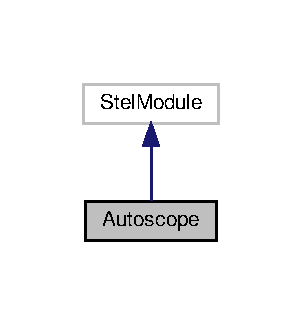
\includegraphics[width=145pt]{class_autoscope__inherit__graph}
\end{center}
\end{figure}


Collaboration diagram for Autoscope\+:
\nopagebreak
\begin{figure}[H]
\begin{center}
\leavevmode
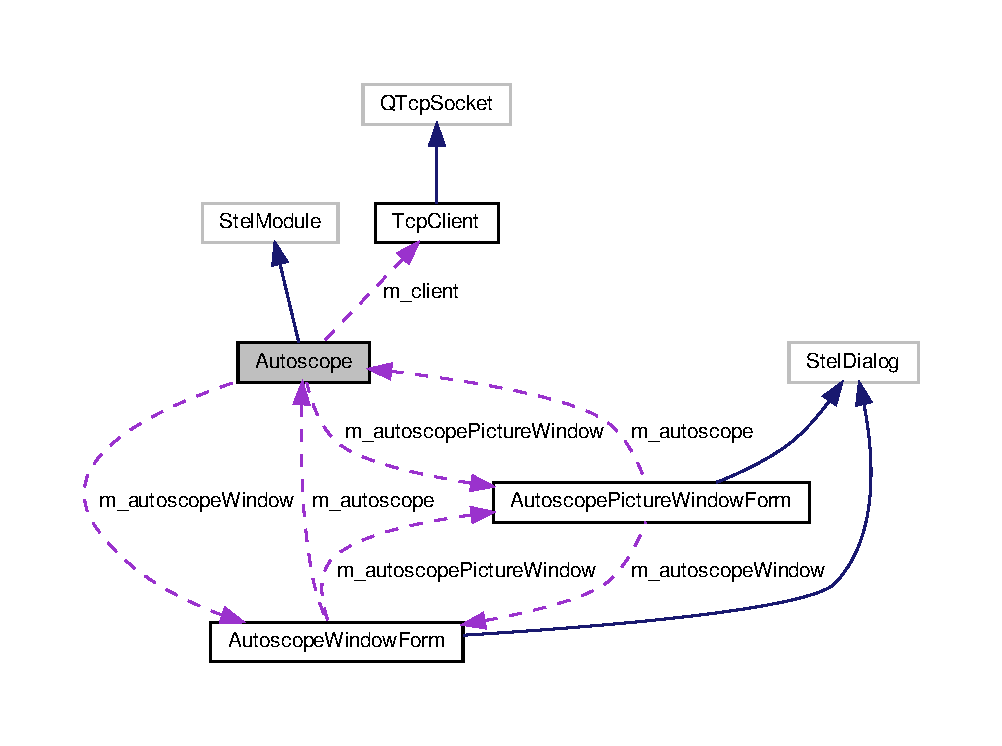
\includegraphics[width=350pt]{class_autoscope__coll__graph}
\end{center}
\end{figure}
\subsection*{Public Slots}
\begin{DoxyCompactItemize}
\item 
void \hyperlink{class_autoscope_a2a3fc7df788580d91949351f687eab7a}{show\+Gui} (void)
\begin{DoxyCompactList}\small\item\em Enable the configuration menu. \end{DoxyCompactList}\item 
void \hyperlink{class_autoscope_ae0c39815fab1084effd39f87e56febf3}{slot\+Track\+Object} (void)
\begin{DoxyCompactList}\small\item\em Start tracking the selected object. \end{DoxyCompactList}\item 
void \hyperlink{class_autoscope_a47d7fbe1a8bcf025ef57b45ead2bcf6e}{slot\+Un\+Track\+Oject} (void)
\begin{DoxyCompactList}\small\item\em Stop tracking the tracked object. \end{DoxyCompactList}\item 
void \hyperlink{class_autoscope_a9216c1ee654d8da28d331b3020b6e27d}{slot\+Enable\+Picture\+Dispaly} (void)
\begin{DoxyCompactList}\small\item\em Toggle the visibility of the picture display. \end{DoxyCompactList}\item 
void \hyperlink{class_autoscope_a55c4956c3a71198b70cf19fea503a776}{slot\+Take\+Picture} (void)
\begin{DoxyCompactList}\small\item\em Send a command to the \hyperlink{class_autoscope}{Autoscope} to take a picture. \end{DoxyCompactList}\item 
void \hyperlink{class_autoscope_ae85d6642b5db861e226a6a261c5c0a37}{slot\+Connected} (void)
\begin{DoxyCompactList}\small\item\em Triggered when the plugin succeed to connect to the \hyperlink{class_autoscope}{Autoscope}. \end{DoxyCompactList}\item 
void \hyperlink{class_autoscope_a7d51e9915c4618d8ee5dd78e5ca079c5}{slot\+Update\+Alt\+Az} (void)
\item 
void \hyperlink{class_autoscope_a191c9746ccdf08bc804150452792b7eb}{slot\+Deconnect\+From\+Autoscope} (void)
\begin{DoxyCompactList}\small\item\em Method used to disconnect the plugin from the \hyperlink{class_autoscope}{Autoscope}. \end{DoxyCompactList}\end{DoxyCompactItemize}
\subsection*{Public Member Functions}
\begin{DoxyCompactItemize}
\item 
\hyperlink{class_autoscope_a70213dc05856f7f6592d089d14f08f68}{Autoscope} ()
\begin{DoxyCompactList}\small\item\em Builder of the \hyperlink{class_autoscope}{Autoscope} class. \end{DoxyCompactList}\item 
virtual \hyperlink{class_autoscope_a8ed25b0eb945f3d2a2a3652322b14b42}{$\sim$\+Autoscope} ()
\begin{DoxyCompactList}\small\item\em Destroyer of the \hyperlink{class_autoscope}{Autoscope} class. \end{DoxyCompactList}\item 
virtual void \hyperlink{class_autoscope_a0aaa7e7edbdd749e209dc42ee360f3a5}{init} ()
\begin{DoxyCompactList}\small\item\em Init method is inherited form Stel\+Module class and is use to initialize components sush as Stel\+Button. \end{DoxyCompactList}\item 
virtual void \hyperlink{class_autoscope_a3def05ed6ebac1d2f0245c96c1719d0a}{update} (double)
\begin{DoxyCompactList}\small\item\em Update method is inherited form Stel\+Module class and is use to update components or methods. It\textquotesingle{}s automatically called by Stel\+Module\+Mgr. \end{DoxyCompactList}\item 
virtual void \hyperlink{class_autoscope_a268e2b524e0abd079f76c55e8443e907}{draw} (Stel\+Core $\ast$core)
\begin{DoxyCompactList}\small\item\em Draw method is inherited form Stel\+Module class and is use to draw components on the user interface. \end{DoxyCompactList}\item 
virtual double \hyperlink{class_autoscope_ad9607f8ffdd72687a19d160a068e1251}{get\+Call\+Order} (Stel\+Module\+Action\+Name action\+Name) const 
\begin{DoxyCompactList}\small\item\em get\+Call\+Order method \end{DoxyCompactList}\item 
virtual bool \hyperlink{class_autoscope_a1a3fca34a12ae80391943194340d2c7e}{configure\+Gui} (bool show)
\begin{DoxyCompactList}\small\item\em Configure\+Gui method is inherited from Stel\+Module class and is use to show the user interface through the plugin manager. \end{DoxyCompactList}\item 
void \hyperlink{class_autoscope_af24c123f39ace0191799b5c20ceca7a6}{load\+Configuration} ()
\begin{DoxyCompactList}\small\item\em Method used to retrieve the configuration of the plugin. \end{DoxyCompactList}\item 
void \hyperlink{class_autoscope_a2c5424afe3270c6069e0109834dd52b5}{restore\+Default\+Configuration} ()
\begin{DoxyCompactList}\small\item\em Method used to restore the default configuration of the plugin. \end{DoxyCompactList}\item 
void \hyperlink{class_autoscope_af61a84b86f02cc55472c53cc79b025b2}{get\+Alt\+Azi} (Stel\+ObjectP object)
\begin{DoxyCompactList}\small\item\em Method used to retrieve the altitude and the azimuth of an object. \end{DoxyCompactList}\item 
Q\+String \hyperlink{class_autoscope_af1d803331f5ab5f5ff5d3839df8952c7}{search\+An\+Object} (Q\+String object\+Name)
\begin{DoxyCompactList}\small\item\em Method used to search an object by it\textquotesingle{}s name. \end{DoxyCompactList}\item 
void \hyperlink{class_autoscope_a0a616d2998641471cb6785e2abb6e7b5}{set\+Track\+Object} (Stel\+ObjectP object)
\begin{DoxyCompactList}\small\item\em Method used to modify the object that the \hyperlink{class_autoscope}{Autoscope} should track. \end{DoxyCompactList}\item 
void \hyperlink{class_autoscope_a5782dc8cf3afeb9710240fdc98d0caa1}{track\+Selected\+Object} (void)
\begin{DoxyCompactList}\small\item\em Method used to tarck the object selected by the user. \end{DoxyCompactList}\item 
Q\+String \hyperlink{class_autoscope_ac5a2819eb2d6971becc544d9f7136b79}{track\+Searched\+Object} (void)
\begin{DoxyCompactList}\small\item\em Method used to tarck the object search by the user. \end{DoxyCompactList}\item 
void \hyperlink{class_autoscope_a2bf2306aa6d3f37dadd83e6e00a35ff3}{clear\+Tracked\+Object} (void)
\begin{DoxyCompactList}\small\item\em Method used to clear the current tracked object. \end{DoxyCompactList}\item 
void \hyperlink{class_autoscope_ac8f9e09385739a5ba5ed460c83ec88df}{move\+Observer\+To\+Object} (Stel\+ObjectP object)
\begin{DoxyCompactList}\small\item\em Method used to move the view in Stellarium to an object. \end{DoxyCompactList}\item 
\hyperlink{class_autoscope_window_form}{Autoscope\+Window\+Form} $\ast$ \hyperlink{class_autoscope_aad8f888c886f1f3e36878e8c3e658813}{get\+Autoscope\+Window} (void)
\begin{DoxyCompactList}\small\item\em Getter which allow any class which have an instance of \hyperlink{class_autoscope}{Autoscope} class to retrieve an instance of the configuration window. \end{DoxyCompactList}\item 
\hyperlink{class_autoscope_picture_window_form}{Autoscope\+Picture\+Window\+Form} $\ast$ \hyperlink{class_autoscope_a78d970ac013a0640bc28cac027737848}{get\+Autoscope\+Picture\+Window} (void)
\begin{DoxyCompactList}\small\item\em Getter which allow any class which have an instance of \hyperlink{class_autoscope}{Autoscope} class to retrieve an instance of the picture window. \end{DoxyCompactList}\item 
\hyperlink{class_command_parser}{Command\+Parser} $\ast$ \hyperlink{class_autoscope_a1be145363f86657b59c6b0cba1497970}{get\+Command\+Parser} (void)
\item 
int \hyperlink{class_autoscope_a0e438a40043c916a7f0f98a30221de11}{get\+Screen\+Width} (void)
\begin{DoxyCompactList}\small\item\em Getter allow any class which have an instance of \hyperlink{class_autoscope}{Autoscope} class to retrieve the width of the screen. \end{DoxyCompactList}\item 
int \hyperlink{class_autoscope_adb579d1e5a23aaa401d5a93be033529d}{get\+Screen\+Height} (void)
\begin{DoxyCompactList}\small\item\em Getter allow any class which have an instance of \hyperlink{class_autoscope}{Autoscope} class to retrieve the height of the screen. \end{DoxyCompactList}\item 
void \hyperlink{class_autoscope_aad5b62b7a114ef8755923067e14f9dd8}{set\+Ip\+Address} (Q\+String addr)
\begin{DoxyCompactList}\small\item\em Setter used to set the IP address of the \hyperlink{class_autoscope}{Autoscope}. \end{DoxyCompactList}\item 
void \hyperlink{class_autoscope_acda88ddee4fb3fbd0333717c0f140e54}{set\+Port} (int port)
\begin{DoxyCompactList}\small\item\em Setter used to set the port of the \hyperlink{class_autoscope}{Autoscope}. \end{DoxyCompactList}\item 
void \hyperlink{class_autoscope_a1ae78f4cada1c4e36f5a06db126017fe}{connect\+To\+Autoscope} (void)
\begin{DoxyCompactList}\small\item\em Method used to connect the plugin to the \hyperlink{class_autoscope}{Autoscope}. \end{DoxyCompactList}\item 
void \hyperlink{class_autoscope_aafe64e11135903a1b83d16ffdd07d63e}{deconnect\+From\+Autoscope} (void)
\begin{DoxyCompactList}\small\item\em Method used to disconnect the plugin from the \hyperlink{class_autoscope}{Autoscope}. \end{DoxyCompactList}\item 
void \hyperlink{class_autoscope_a724178eb130dde22dc564a086b82c0e4}{send\+To\+Server} (Q\+String)
\end{DoxyCompactItemize}
\subsection*{Public Attributes}
\begin{DoxyCompactItemize}
\item 
Stel\+Movement\+Mgr $\ast$ \hyperlink{class_autoscope_ab34124a1179a937ac061bb4fa3faa2de}{mv\+Mgr}
\begin{DoxyCompactList}\small\item\em An instance of Stellarium movement manager and it\textquotesingle{}s use to move the view in Stellarium. \end{DoxyCompactList}\item 
Stel\+Object\+Mgr $\ast$ \hyperlink{class_autoscope_aec2c452e45c0a7d045417a8656aa7c45}{object\+Mgr}
\begin{DoxyCompactList}\small\item\em An instance of Stellarium object manager and it\textquotesingle{}s use to retrieve selected object or search object by name. \end{DoxyCompactList}\end{DoxyCompactItemize}
\subsection*{Private Attributes}
\begin{DoxyCompactItemize}
\item 
Q\+Settings $\ast$ \hyperlink{class_autoscope_a6a17eb00225f765623844eaa9f80e71e}{conf}
\item 
Stel\+Gui $\ast$ \hyperlink{class_autoscope_a90c44f576ab3acd74da3af3ad8162ca7}{gui}
\item 
\hyperlink{class_autoscope_window_form}{Autoscope\+Window\+Form} $\ast$ \hyperlink{class_autoscope_a33104164061c784c65c1f94bfde26423}{m\+\_\+autoscope\+Window}
\begin{DoxyCompactList}\small\item\em An instance of \hyperlink{class_autoscope_window_form}{Autoscope\+Window\+Form} class. \end{DoxyCompactList}\item 
\hyperlink{class_autoscope_picture_window_form}{Autoscope\+Picture\+Window\+Form} $\ast$ \hyperlink{class_autoscope_a75a50ab46f25c007b9a86d3776385fc6}{m\+\_\+autoscope\+Picture\+Window}
\begin{DoxyCompactList}\small\item\em An instance of \hyperlink{class_autoscope_picture_window_form}{Autoscope\+Picture\+Window\+Form} class. \end{DoxyCompactList}\item 
Stel\+Core $\ast$ \hyperlink{class_autoscope_aa333cfe8f256f5698c686423cad648c2}{m\+\_\+core}
\begin{DoxyCompactList}\small\item\em An instance of Stel\+Core. \end{DoxyCompactList}\item 
Q\+Timer $\ast$ \hyperlink{class_autoscope_a6d86ef1f5ea17f5175009a15004b2459}{m\+\_\+timer}
\item 
\hyperlink{class_command_parser}{Command\+Parser} $\ast$ \hyperlink{class_autoscope_ab4a9bf62ccbcf24b4a6e3752cff9f090}{m\+\_\+parser}
\item 
Vec3f \hyperlink{class_autoscope_a58327daadc555f31fc62b6db85e3fcfa}{mark\+Color}
\item 
Linear\+Fader \hyperlink{class_autoscope_a9c141894e06ed64f4131f1071e9e18af}{mark\+Fader}
\item 
bool \hyperlink{class_autoscope_a8c066a069946815c05fe7d32b13211d3}{displayed\+At\+Startup}
\item 
bool \hyperlink{class_autoscope_ac995550136b93293df166aead2eda5b7}{gui\+Is\+Visible} = false
\item 
Stel\+Button $\ast$ \hyperlink{class_autoscope_a5b14962697fbd8fffac986df08aee611}{menu\+Button}
\item 
Stel\+Button $\ast$ \hyperlink{class_autoscope_a816e3212639b4204e9917704e02b0d09}{track\+Button}
\item 
Stel\+Button $\ast$ \hyperlink{class_autoscope_a5d3be6a8522dc18b921936b57c8e661c}{un\+Track\+Button}
\item 
Stel\+Button $\ast$ \hyperlink{class_autoscope_aa3b4663ded25875ce8fb21906b38d174}{Enable\+Picture\+Display}
\item 
Stel\+Button $\ast$ \hyperlink{class_autoscope_a8f64e1d50e979751403a70008f0d01da}{take\+Picture}
\item 
Q\+Font \hyperlink{class_autoscope_a168d6d47f412a7966c2f5ddeb0f4cc79}{font}
\item 
Stel\+ObjectP \hyperlink{class_autoscope_a5bcfda333996f4fc3a959306be3e3d07}{Sun}
\item 
Stel\+ObjectP \hyperlink{class_autoscope_a170fbbc7b2a719517912aa3614727021}{track\+Object}
\item 
Stel\+ObjectP \hyperlink{class_autoscope_a954a97691346ff2fb0981877554c1ac3}{selected\+Object}
\item 
Stel\+ObjectP \hyperlink{class_autoscope_aba59abee95b4b5443709dce1d61a3498}{searched\+Object}
\item 
Vec3d \hyperlink{class_autoscope_aff4d8365cc96689c79f3370ebde45b9e}{object\+Position}
\item 
Q\+List$<$ Stel\+ObjectP $>$ \hyperlink{class_autoscope_aa02f096fc07e27ef3843eb4f8ba2c5a5}{new\+Selected}
\item 
bool \hyperlink{class_autoscope_adcd9ee42b339c3c526231ed97c0ef6fa}{search\+Object\+Found} = false
\item 
int \hyperlink{class_autoscope_afe92778dfed037b0ec41ad51f8086a56}{m\+\_\+screen\+Width}
\item 
int \hyperlink{class_autoscope_a003c73a069f579f831eeaa8f04cf2977}{m\+\_\+screen\+Height}
\item 
\hyperlink{class_tcp_client}{Tcp\+Client} $\ast$ \hyperlink{class_autoscope_af6e7a8d7cf7014e9b0f9296e2b7d7fd5}{m\+\_\+client}
\begin{DoxyCompactList}\small\item\em An instance of \hyperlink{class_tcp_client}{Tcp\+Client} class. \end{DoxyCompactList}\item 
Q\+Host\+Address \hyperlink{class_autoscope_aa3c1b8d19881d76c680b8c4ea1692c89}{m\+\_\+autoscope\+Ip}
\item 
int \hyperlink{class_autoscope_abb67968cc6c6678995512aa1a05ad0e1}{m\+\_\+autoscope\+Port} = 4444
\end{DoxyCompactItemize}


\subsection{Detailed Description}
This class is use to retrieve and compute data for sending to the telescope, and call user interfaces windows. 

\subsection{Constructor \& Destructor Documentation}
\index{Autoscope@{Autoscope}!Autoscope@{Autoscope}}
\index{Autoscope@{Autoscope}!Autoscope@{Autoscope}}
\subsubsection[{\texorpdfstring{Autoscope()}{Autoscope()}}]{\setlength{\rightskip}{0pt plus 5cm}Autoscope\+::\+Autoscope (
\begin{DoxyParamCaption}
{}
\end{DoxyParamCaption}
)}\hypertarget{class_autoscope_a70213dc05856f7f6592d089d14f08f68}{}\label{class_autoscope_a70213dc05856f7f6592d089d14f08f68}


Builder of the \hyperlink{class_autoscope}{Autoscope} class. 

\index{Autoscope@{Autoscope}!````~Autoscope@{$\sim$\+Autoscope}}
\index{````~Autoscope@{$\sim$\+Autoscope}!Autoscope@{Autoscope}}
\subsubsection[{\texorpdfstring{$\sim$\+Autoscope()}{~Autoscope()}}]{\setlength{\rightskip}{0pt plus 5cm}Autoscope\+::$\sim$\+Autoscope (
\begin{DoxyParamCaption}
{}
\end{DoxyParamCaption}
)\hspace{0.3cm}{\ttfamily [virtual]}}\hypertarget{class_autoscope_a8ed25b0eb945f3d2a2a3652322b14b42}{}\label{class_autoscope_a8ed25b0eb945f3d2a2a3652322b14b42}


Destroyer of the \hyperlink{class_autoscope}{Autoscope} class. 



\subsection{Member Function Documentation}
\index{Autoscope@{Autoscope}!clear\+Tracked\+Object@{clear\+Tracked\+Object}}
\index{clear\+Tracked\+Object@{clear\+Tracked\+Object}!Autoscope@{Autoscope}}
\subsubsection[{\texorpdfstring{clear\+Tracked\+Object(void)}{clearTrackedObject(void)}}]{\setlength{\rightskip}{0pt plus 5cm}void Autoscope\+::clear\+Tracked\+Object (
\begin{DoxyParamCaption}
\item[{void}]{}
\end{DoxyParamCaption}
)}\hypertarget{class_autoscope_a2bf2306aa6d3f37dadd83e6e00a35ff3}{}\label{class_autoscope_a2bf2306aa6d3f37dadd83e6e00a35ff3}


Method used to clear the current tracked object. 

\index{Autoscope@{Autoscope}!configure\+Gui@{configure\+Gui}}
\index{configure\+Gui@{configure\+Gui}!Autoscope@{Autoscope}}
\subsubsection[{\texorpdfstring{configure\+Gui(bool show)}{configureGui(bool show)}}]{\setlength{\rightskip}{0pt plus 5cm}bool Autoscope\+::configure\+Gui (
\begin{DoxyParamCaption}
\item[{bool}]{show}
\end{DoxyParamCaption}
)\hspace{0.3cm}{\ttfamily [virtual]}}\hypertarget{class_autoscope_a1a3fca34a12ae80391943194340d2c7e}{}\label{class_autoscope_a1a3fca34a12ae80391943194340d2c7e}


Configure\+Gui method is inherited from Stel\+Module class and is use to show the user interface through the plugin manager. 


\begin{DoxyParams}{Parameters}
{\em show} & If show is true, set the gui visible, else set it invisible \\
\hline
\end{DoxyParams}
\begin{DoxyReturn}{Returns}
true if it doesn\textquotesingle{}t crash! 
\end{DoxyReturn}
\begin{DoxySeeAlso}{See also}
Stel\+Module 
\end{DoxySeeAlso}
\index{Autoscope@{Autoscope}!connect\+To\+Autoscope@{connect\+To\+Autoscope}}
\index{connect\+To\+Autoscope@{connect\+To\+Autoscope}!Autoscope@{Autoscope}}
\subsubsection[{\texorpdfstring{connect\+To\+Autoscope(void)}{connectToAutoscope(void)}}]{\setlength{\rightskip}{0pt plus 5cm}void Autoscope\+::connect\+To\+Autoscope (
\begin{DoxyParamCaption}
\item[{void}]{}
\end{DoxyParamCaption}
)}\hypertarget{class_autoscope_a1ae78f4cada1c4e36f5a06db126017fe}{}\label{class_autoscope_a1ae78f4cada1c4e36f5a06db126017fe}


Method used to connect the plugin to the \hyperlink{class_autoscope}{Autoscope}. 

\index{Autoscope@{Autoscope}!deconnect\+From\+Autoscope@{deconnect\+From\+Autoscope}}
\index{deconnect\+From\+Autoscope@{deconnect\+From\+Autoscope}!Autoscope@{Autoscope}}
\subsubsection[{\texorpdfstring{deconnect\+From\+Autoscope(void)}{deconnectFromAutoscope(void)}}]{\setlength{\rightskip}{0pt plus 5cm}void Autoscope\+::deconnect\+From\+Autoscope (
\begin{DoxyParamCaption}
\item[{void}]{}
\end{DoxyParamCaption}
)}\hypertarget{class_autoscope_aafe64e11135903a1b83d16ffdd07d63e}{}\label{class_autoscope_aafe64e11135903a1b83d16ffdd07d63e}


Method used to disconnect the plugin from the \hyperlink{class_autoscope}{Autoscope}. 

\index{Autoscope@{Autoscope}!draw@{draw}}
\index{draw@{draw}!Autoscope@{Autoscope}}
\subsubsection[{\texorpdfstring{draw(\+Stel\+Core $\ast$core)}{draw(StelCore *core)}}]{\setlength{\rightskip}{0pt plus 5cm}void Autoscope\+::draw (
\begin{DoxyParamCaption}
\item[{Stel\+Core $\ast$}]{core}
\end{DoxyParamCaption}
)\hspace{0.3cm}{\ttfamily [virtual]}}\hypertarget{class_autoscope_a268e2b524e0abd079f76c55e8443e907}{}\label{class_autoscope_a268e2b524e0abd079f76c55e8443e907}


Draw method is inherited form Stel\+Module class and is use to draw components on the user interface. 


\begin{DoxyParams}{Parameters}
{\em core} & The object given by Stel\+Module\+Mgr to draw forms \\
\hline
\end{DoxyParams}
\begin{DoxySeeAlso}{See also}
Stel\+Module 
\end{DoxySeeAlso}
\index{Autoscope@{Autoscope}!get\+Alt\+Azi@{get\+Alt\+Azi}}
\index{get\+Alt\+Azi@{get\+Alt\+Azi}!Autoscope@{Autoscope}}
\subsubsection[{\texorpdfstring{get\+Alt\+Azi(\+Stel\+Object\+P object)}{getAltAzi(StelObjectP object)}}]{\setlength{\rightskip}{0pt plus 5cm}void Autoscope\+::get\+Alt\+Azi (
\begin{DoxyParamCaption}
\item[{Stel\+ObjectP}]{object}
\end{DoxyParamCaption}
)}\hypertarget{class_autoscope_af61a84b86f02cc55472c53cc79b025b2}{}\label{class_autoscope_af61a84b86f02cc55472c53cc79b025b2}


Method used to retrieve the altitude and the azimuth of an object. 


\begin{DoxyParams}{Parameters}
{\em object} & The object that we want to retrieve data from \\
\hline
\end{DoxyParams}
\index{Autoscope@{Autoscope}!get\+Autoscope\+Picture\+Window@{get\+Autoscope\+Picture\+Window}}
\index{get\+Autoscope\+Picture\+Window@{get\+Autoscope\+Picture\+Window}!Autoscope@{Autoscope}}
\subsubsection[{\texorpdfstring{get\+Autoscope\+Picture\+Window(void)}{getAutoscopePictureWindow(void)}}]{\setlength{\rightskip}{0pt plus 5cm}{\bf Autoscope\+Picture\+Window\+Form}$\ast$ Autoscope\+::get\+Autoscope\+Picture\+Window (
\begin{DoxyParamCaption}
\item[{void}]{}
\end{DoxyParamCaption}
)\hspace{0.3cm}{\ttfamily [inline]}}\hypertarget{class_autoscope_a78d970ac013a0640bc28cac027737848}{}\label{class_autoscope_a78d970ac013a0640bc28cac027737848}


Getter which allow any class which have an instance of \hyperlink{class_autoscope}{Autoscope} class to retrieve an instance of the picture window. 

\begin{DoxyReturn}{Returns}
An instance of the picture window 
\end{DoxyReturn}
\index{Autoscope@{Autoscope}!get\+Autoscope\+Window@{get\+Autoscope\+Window}}
\index{get\+Autoscope\+Window@{get\+Autoscope\+Window}!Autoscope@{Autoscope}}
\subsubsection[{\texorpdfstring{get\+Autoscope\+Window(void)}{getAutoscopeWindow(void)}}]{\setlength{\rightskip}{0pt plus 5cm}{\bf Autoscope\+Window\+Form}$\ast$ Autoscope\+::get\+Autoscope\+Window (
\begin{DoxyParamCaption}
\item[{void}]{}
\end{DoxyParamCaption}
)\hspace{0.3cm}{\ttfamily [inline]}}\hypertarget{class_autoscope_aad8f888c886f1f3e36878e8c3e658813}{}\label{class_autoscope_aad8f888c886f1f3e36878e8c3e658813}


Getter which allow any class which have an instance of \hyperlink{class_autoscope}{Autoscope} class to retrieve an instance of the configuration window. 

\begin{DoxyReturn}{Returns}
An instance of the configuration window 
\end{DoxyReturn}
\index{Autoscope@{Autoscope}!get\+Call\+Order@{get\+Call\+Order}}
\index{get\+Call\+Order@{get\+Call\+Order}!Autoscope@{Autoscope}}
\subsubsection[{\texorpdfstring{get\+Call\+Order(\+Stel\+Module\+Action\+Name action\+Name) const }{getCallOrder(StelModuleActionName actionName) const }}]{\setlength{\rightskip}{0pt plus 5cm}double Autoscope\+::get\+Call\+Order (
\begin{DoxyParamCaption}
\item[{Stel\+Module\+Action\+Name}]{action\+Name}
\end{DoxyParamCaption}
) const\hspace{0.3cm}{\ttfamily [virtual]}}\hypertarget{class_autoscope_ad9607f8ffdd72687a19d160a068e1251}{}\label{class_autoscope_ad9607f8ffdd72687a19d160a068e1251}


get\+Call\+Order method 


\begin{DoxyParams}{Parameters}
{\em action\+Name} & \\
\hline
\end{DoxyParams}
\begin{DoxySeeAlso}{See also}
Stel\+Module 
\end{DoxySeeAlso}
\begin{DoxyReturn}{Returns}

\end{DoxyReturn}
\index{Autoscope@{Autoscope}!get\+Command\+Parser@{get\+Command\+Parser}}
\index{get\+Command\+Parser@{get\+Command\+Parser}!Autoscope@{Autoscope}}
\subsubsection[{\texorpdfstring{get\+Command\+Parser(void)}{getCommandParser(void)}}]{\setlength{\rightskip}{0pt plus 5cm}{\bf Command\+Parser}$\ast$ Autoscope\+::get\+Command\+Parser (
\begin{DoxyParamCaption}
\item[{void}]{}
\end{DoxyParamCaption}
)\hspace{0.3cm}{\ttfamily [inline]}}\hypertarget{class_autoscope_a1be145363f86657b59c6b0cba1497970}{}\label{class_autoscope_a1be145363f86657b59c6b0cba1497970}
\index{Autoscope@{Autoscope}!get\+Screen\+Height@{get\+Screen\+Height}}
\index{get\+Screen\+Height@{get\+Screen\+Height}!Autoscope@{Autoscope}}
\subsubsection[{\texorpdfstring{get\+Screen\+Height(void)}{getScreenHeight(void)}}]{\setlength{\rightskip}{0pt plus 5cm}int Autoscope\+::get\+Screen\+Height (
\begin{DoxyParamCaption}
\item[{void}]{}
\end{DoxyParamCaption}
)\hspace{0.3cm}{\ttfamily [inline]}}\hypertarget{class_autoscope_adb579d1e5a23aaa401d5a93be033529d}{}\label{class_autoscope_adb579d1e5a23aaa401d5a93be033529d}


Getter allow any class which have an instance of \hyperlink{class_autoscope}{Autoscope} class to retrieve the height of the screen. 

\begin{DoxyReturn}{Returns}
The height of the screen 
\end{DoxyReturn}
\index{Autoscope@{Autoscope}!get\+Screen\+Width@{get\+Screen\+Width}}
\index{get\+Screen\+Width@{get\+Screen\+Width}!Autoscope@{Autoscope}}
\subsubsection[{\texorpdfstring{get\+Screen\+Width(void)}{getScreenWidth(void)}}]{\setlength{\rightskip}{0pt plus 5cm}int Autoscope\+::get\+Screen\+Width (
\begin{DoxyParamCaption}
\item[{void}]{}
\end{DoxyParamCaption}
)\hspace{0.3cm}{\ttfamily [inline]}}\hypertarget{class_autoscope_a0e438a40043c916a7f0f98a30221de11}{}\label{class_autoscope_a0e438a40043c916a7f0f98a30221de11}


Getter allow any class which have an instance of \hyperlink{class_autoscope}{Autoscope} class to retrieve the width of the screen. 

\begin{DoxyReturn}{Returns}
The width of the screen 
\end{DoxyReturn}
\index{Autoscope@{Autoscope}!init@{init}}
\index{init@{init}!Autoscope@{Autoscope}}
\subsubsection[{\texorpdfstring{init()}{init()}}]{\setlength{\rightskip}{0pt plus 5cm}void Autoscope\+::init (
\begin{DoxyParamCaption}
{}
\end{DoxyParamCaption}
)\hspace{0.3cm}{\ttfamily [virtual]}}\hypertarget{class_autoscope_a0aaa7e7edbdd749e209dc42ee360f3a5}{}\label{class_autoscope_a0aaa7e7edbdd749e209dc42ee360f3a5}


Init method is inherited form Stel\+Module class and is use to initialize components sush as Stel\+Button. 

\begin{DoxySeeAlso}{See also}
Stel\+Module 
\end{DoxySeeAlso}
\index{Autoscope@{Autoscope}!load\+Configuration@{load\+Configuration}}
\index{load\+Configuration@{load\+Configuration}!Autoscope@{Autoscope}}
\subsubsection[{\texorpdfstring{load\+Configuration()}{loadConfiguration()}}]{\setlength{\rightskip}{0pt plus 5cm}void Autoscope\+::load\+Configuration (
\begin{DoxyParamCaption}
{}
\end{DoxyParamCaption}
)}\hypertarget{class_autoscope_af24c123f39ace0191799b5c20ceca7a6}{}\label{class_autoscope_af24c123f39ace0191799b5c20ceca7a6}


Method used to retrieve the configuration of the plugin. 

\index{Autoscope@{Autoscope}!move\+Observer\+To\+Object@{move\+Observer\+To\+Object}}
\index{move\+Observer\+To\+Object@{move\+Observer\+To\+Object}!Autoscope@{Autoscope}}
\subsubsection[{\texorpdfstring{move\+Observer\+To\+Object(\+Stel\+Object\+P object)}{moveObserverToObject(StelObjectP object)}}]{\setlength{\rightskip}{0pt plus 5cm}void Autoscope\+::move\+Observer\+To\+Object (
\begin{DoxyParamCaption}
\item[{Stel\+ObjectP}]{object}
\end{DoxyParamCaption}
)}\hypertarget{class_autoscope_ac8f9e09385739a5ba5ed460c83ec88df}{}\label{class_autoscope_ac8f9e09385739a5ba5ed460c83ec88df}


Method used to move the view in Stellarium to an object. 


\begin{DoxyParams}{Parameters}
{\em object} & \\
\hline
\end{DoxyParams}
\index{Autoscope@{Autoscope}!restore\+Default\+Configuration@{restore\+Default\+Configuration}}
\index{restore\+Default\+Configuration@{restore\+Default\+Configuration}!Autoscope@{Autoscope}}
\subsubsection[{\texorpdfstring{restore\+Default\+Configuration()}{restoreDefaultConfiguration()}}]{\setlength{\rightskip}{0pt plus 5cm}void Autoscope\+::restore\+Default\+Configuration (
\begin{DoxyParamCaption}
{}
\end{DoxyParamCaption}
)}\hypertarget{class_autoscope_a2c5424afe3270c6069e0109834dd52b5}{}\label{class_autoscope_a2c5424afe3270c6069e0109834dd52b5}


Method used to restore the default configuration of the plugin. 

\index{Autoscope@{Autoscope}!search\+An\+Object@{search\+An\+Object}}
\index{search\+An\+Object@{search\+An\+Object}!Autoscope@{Autoscope}}
\subsubsection[{\texorpdfstring{search\+An\+Object(\+Q\+String object\+Name)}{searchAnObject(QString objectName)}}]{\setlength{\rightskip}{0pt plus 5cm}Q\+String Autoscope\+::search\+An\+Object (
\begin{DoxyParamCaption}
\item[{Q\+String}]{object\+Name}
\end{DoxyParamCaption}
)}\hypertarget{class_autoscope_af1d803331f5ab5f5ff5d3839df8952c7}{}\label{class_autoscope_af1d803331f5ab5f5ff5d3839df8952c7}


Method used to search an object by it\textquotesingle{}s name. 


\begin{DoxyParams}{Parameters}
{\em object\+Name} & The name of the object \\
\hline
\end{DoxyParams}
\begin{DoxyReturn}{Returns}
A string to display in the search\+Messenger 
\end{DoxyReturn}
\index{Autoscope@{Autoscope}!send\+To\+Server@{send\+To\+Server}}
\index{send\+To\+Server@{send\+To\+Server}!Autoscope@{Autoscope}}
\subsubsection[{\texorpdfstring{send\+To\+Server(\+Q\+String)}{sendToServer(QString)}}]{\setlength{\rightskip}{0pt plus 5cm}void Autoscope\+::send\+To\+Server (
\begin{DoxyParamCaption}
\item[{Q\+String}]{str}
\end{DoxyParamCaption}
)}\hypertarget{class_autoscope_a724178eb130dde22dc564a086b82c0e4}{}\label{class_autoscope_a724178eb130dde22dc564a086b82c0e4}
\index{Autoscope@{Autoscope}!set\+Ip\+Address@{set\+Ip\+Address}}
\index{set\+Ip\+Address@{set\+Ip\+Address}!Autoscope@{Autoscope}}
\subsubsection[{\texorpdfstring{set\+Ip\+Address(\+Q\+String addr)}{setIpAddress(QString addr)}}]{\setlength{\rightskip}{0pt plus 5cm}void Autoscope\+::set\+Ip\+Address (
\begin{DoxyParamCaption}
\item[{Q\+String}]{addr}
\end{DoxyParamCaption}
)\hspace{0.3cm}{\ttfamily [inline]}}\hypertarget{class_autoscope_aad5b62b7a114ef8755923067e14f9dd8}{}\label{class_autoscope_aad5b62b7a114ef8755923067e14f9dd8}


Setter used to set the IP address of the \hyperlink{class_autoscope}{Autoscope}. 


\begin{DoxyParams}{Parameters}
{\em addr} & The IP address of the \hyperlink{class_autoscope}{Autoscope} \\
\hline
\end{DoxyParams}
\index{Autoscope@{Autoscope}!set\+Port@{set\+Port}}
\index{set\+Port@{set\+Port}!Autoscope@{Autoscope}}
\subsubsection[{\texorpdfstring{set\+Port(int port)}{setPort(int port)}}]{\setlength{\rightskip}{0pt plus 5cm}void Autoscope\+::set\+Port (
\begin{DoxyParamCaption}
\item[{int}]{port}
\end{DoxyParamCaption}
)\hspace{0.3cm}{\ttfamily [inline]}}\hypertarget{class_autoscope_acda88ddee4fb3fbd0333717c0f140e54}{}\label{class_autoscope_acda88ddee4fb3fbd0333717c0f140e54}


Setter used to set the port of the \hyperlink{class_autoscope}{Autoscope}. 


\begin{DoxyParams}{Parameters}
{\em port} & The port of the \hyperlink{class_autoscope}{Autoscope} \\
\hline
\end{DoxyParams}
\index{Autoscope@{Autoscope}!set\+Track\+Object@{set\+Track\+Object}}
\index{set\+Track\+Object@{set\+Track\+Object}!Autoscope@{Autoscope}}
\subsubsection[{\texorpdfstring{set\+Track\+Object(\+Stel\+Object\+P object)}{setTrackObject(StelObjectP object)}}]{\setlength{\rightskip}{0pt plus 5cm}void Autoscope\+::set\+Track\+Object (
\begin{DoxyParamCaption}
\item[{Stel\+ObjectP}]{object}
\end{DoxyParamCaption}
)}\hypertarget{class_autoscope_a0a616d2998641471cb6785e2abb6e7b5}{}\label{class_autoscope_a0a616d2998641471cb6785e2abb6e7b5}


Method used to modify the object that the \hyperlink{class_autoscope}{Autoscope} should track. 


\begin{DoxyParams}{Parameters}
{\em object} & The object to track \\
\hline
\end{DoxyParams}
\index{Autoscope@{Autoscope}!show\+Gui@{show\+Gui}}
\index{show\+Gui@{show\+Gui}!Autoscope@{Autoscope}}
\subsubsection[{\texorpdfstring{show\+Gui}{showGui}}]{\setlength{\rightskip}{0pt plus 5cm}void Autoscope\+::show\+Gui (
\begin{DoxyParamCaption}
\item[{void}]{}
\end{DoxyParamCaption}
)\hspace{0.3cm}{\ttfamily [slot]}}\hypertarget{class_autoscope_a2a3fc7df788580d91949351f687eab7a}{}\label{class_autoscope_a2a3fc7df788580d91949351f687eab7a}


Enable the configuration menu. 

\index{Autoscope@{Autoscope}!slot\+Connected@{slot\+Connected}}
\index{slot\+Connected@{slot\+Connected}!Autoscope@{Autoscope}}
\subsubsection[{\texorpdfstring{slot\+Connected}{slotConnected}}]{\setlength{\rightskip}{0pt plus 5cm}void Autoscope\+::slot\+Connected (
\begin{DoxyParamCaption}
\item[{void}]{}
\end{DoxyParamCaption}
)\hspace{0.3cm}{\ttfamily [slot]}}\hypertarget{class_autoscope_ae85d6642b5db861e226a6a261c5c0a37}{}\label{class_autoscope_ae85d6642b5db861e226a6a261c5c0a37}


Triggered when the plugin succeed to connect to the \hyperlink{class_autoscope}{Autoscope}. 

\index{Autoscope@{Autoscope}!slot\+Deconnect\+From\+Autoscope@{slot\+Deconnect\+From\+Autoscope}}
\index{slot\+Deconnect\+From\+Autoscope@{slot\+Deconnect\+From\+Autoscope}!Autoscope@{Autoscope}}
\subsubsection[{\texorpdfstring{slot\+Deconnect\+From\+Autoscope}{slotDeconnectFromAutoscope}}]{\setlength{\rightskip}{0pt plus 5cm}void Autoscope\+::slot\+Deconnect\+From\+Autoscope (
\begin{DoxyParamCaption}
\item[{void}]{}
\end{DoxyParamCaption}
)\hspace{0.3cm}{\ttfamily [slot]}}\hypertarget{class_autoscope_a191c9746ccdf08bc804150452792b7eb}{}\label{class_autoscope_a191c9746ccdf08bc804150452792b7eb}


Method used to disconnect the plugin from the \hyperlink{class_autoscope}{Autoscope}. 

\index{Autoscope@{Autoscope}!slot\+Enable\+Picture\+Dispaly@{slot\+Enable\+Picture\+Dispaly}}
\index{slot\+Enable\+Picture\+Dispaly@{slot\+Enable\+Picture\+Dispaly}!Autoscope@{Autoscope}}
\subsubsection[{\texorpdfstring{slot\+Enable\+Picture\+Dispaly}{slotEnablePictureDispaly}}]{\setlength{\rightskip}{0pt plus 5cm}void Autoscope\+::slot\+Enable\+Picture\+Dispaly (
\begin{DoxyParamCaption}
\item[{void}]{}
\end{DoxyParamCaption}
)\hspace{0.3cm}{\ttfamily [slot]}}\hypertarget{class_autoscope_a9216c1ee654d8da28d331b3020b6e27d}{}\label{class_autoscope_a9216c1ee654d8da28d331b3020b6e27d}


Toggle the visibility of the picture display. 

\index{Autoscope@{Autoscope}!slot\+Take\+Picture@{slot\+Take\+Picture}}
\index{slot\+Take\+Picture@{slot\+Take\+Picture}!Autoscope@{Autoscope}}
\subsubsection[{\texorpdfstring{slot\+Take\+Picture}{slotTakePicture}}]{\setlength{\rightskip}{0pt plus 5cm}void Autoscope\+::slot\+Take\+Picture (
\begin{DoxyParamCaption}
\item[{void}]{}
\end{DoxyParamCaption}
)\hspace{0.3cm}{\ttfamily [slot]}}\hypertarget{class_autoscope_a55c4956c3a71198b70cf19fea503a776}{}\label{class_autoscope_a55c4956c3a71198b70cf19fea503a776}


Send a command to the \hyperlink{class_autoscope}{Autoscope} to take a picture. 

\index{Autoscope@{Autoscope}!slot\+Track\+Object@{slot\+Track\+Object}}
\index{slot\+Track\+Object@{slot\+Track\+Object}!Autoscope@{Autoscope}}
\subsubsection[{\texorpdfstring{slot\+Track\+Object}{slotTrackObject}}]{\setlength{\rightskip}{0pt plus 5cm}void Autoscope\+::slot\+Track\+Object (
\begin{DoxyParamCaption}
\item[{void}]{}
\end{DoxyParamCaption}
)\hspace{0.3cm}{\ttfamily [slot]}}\hypertarget{class_autoscope_ae0c39815fab1084effd39f87e56febf3}{}\label{class_autoscope_ae0c39815fab1084effd39f87e56febf3}


Start tracking the selected object. 

\index{Autoscope@{Autoscope}!slot\+Un\+Track\+Oject@{slot\+Un\+Track\+Oject}}
\index{slot\+Un\+Track\+Oject@{slot\+Un\+Track\+Oject}!Autoscope@{Autoscope}}
\subsubsection[{\texorpdfstring{slot\+Un\+Track\+Oject}{slotUnTrackOject}}]{\setlength{\rightskip}{0pt plus 5cm}void Autoscope\+::slot\+Un\+Track\+Oject (
\begin{DoxyParamCaption}
\item[{void}]{}
\end{DoxyParamCaption}
)\hspace{0.3cm}{\ttfamily [slot]}}\hypertarget{class_autoscope_a47d7fbe1a8bcf025ef57b45ead2bcf6e}{}\label{class_autoscope_a47d7fbe1a8bcf025ef57b45ead2bcf6e}


Stop tracking the tracked object. 

\index{Autoscope@{Autoscope}!slot\+Update\+Alt\+Az@{slot\+Update\+Alt\+Az}}
\index{slot\+Update\+Alt\+Az@{slot\+Update\+Alt\+Az}!Autoscope@{Autoscope}}
\subsubsection[{\texorpdfstring{slot\+Update\+Alt\+Az}{slotUpdateAltAz}}]{\setlength{\rightskip}{0pt plus 5cm}void Autoscope\+::slot\+Update\+Alt\+Az (
\begin{DoxyParamCaption}
\item[{void}]{}
\end{DoxyParamCaption}
)\hspace{0.3cm}{\ttfamily [slot]}}\hypertarget{class_autoscope_a7d51e9915c4618d8ee5dd78e5ca079c5}{}\label{class_autoscope_a7d51e9915c4618d8ee5dd78e5ca079c5}
\index{Autoscope@{Autoscope}!track\+Searched\+Object@{track\+Searched\+Object}}
\index{track\+Searched\+Object@{track\+Searched\+Object}!Autoscope@{Autoscope}}
\subsubsection[{\texorpdfstring{track\+Searched\+Object(void)}{trackSearchedObject(void)}}]{\setlength{\rightskip}{0pt plus 5cm}Q\+String Autoscope\+::track\+Searched\+Object (
\begin{DoxyParamCaption}
\item[{void}]{}
\end{DoxyParamCaption}
)}\hypertarget{class_autoscope_ac5a2819eb2d6971becc544d9f7136b79}{}\label{class_autoscope_ac5a2819eb2d6971becc544d9f7136b79}


Method used to tarck the object search by the user. 

\begin{DoxyReturn}{Returns}
A string to display in the search\+Messenger 
\end{DoxyReturn}
\index{Autoscope@{Autoscope}!track\+Selected\+Object@{track\+Selected\+Object}}
\index{track\+Selected\+Object@{track\+Selected\+Object}!Autoscope@{Autoscope}}
\subsubsection[{\texorpdfstring{track\+Selected\+Object(void)}{trackSelectedObject(void)}}]{\setlength{\rightskip}{0pt plus 5cm}void Autoscope\+::track\+Selected\+Object (
\begin{DoxyParamCaption}
\item[{void}]{}
\end{DoxyParamCaption}
)}\hypertarget{class_autoscope_a5782dc8cf3afeb9710240fdc98d0caa1}{}\label{class_autoscope_a5782dc8cf3afeb9710240fdc98d0caa1}


Method used to tarck the object selected by the user. 

\index{Autoscope@{Autoscope}!update@{update}}
\index{update@{update}!Autoscope@{Autoscope}}
\subsubsection[{\texorpdfstring{update(double)}{update(double)}}]{\setlength{\rightskip}{0pt plus 5cm}void Autoscope\+::update (
\begin{DoxyParamCaption}
\item[{double}]{t}
\end{DoxyParamCaption}
)\hspace{0.3cm}{\ttfamily [virtual]}}\hypertarget{class_autoscope_a3def05ed6ebac1d2f0245c96c1719d0a}{}\label{class_autoscope_a3def05ed6ebac1d2f0245c96c1719d0a}


Update method is inherited form Stel\+Module class and is use to update components or methods. It\textquotesingle{}s automatically called by Stel\+Module\+Mgr. 

\begin{DoxySeeAlso}{See also}
Stel\+Module 
\end{DoxySeeAlso}


\subsection{Member Data Documentation}
\index{Autoscope@{Autoscope}!conf@{conf}}
\index{conf@{conf}!Autoscope@{Autoscope}}
\subsubsection[{\texorpdfstring{conf}{conf}}]{\setlength{\rightskip}{0pt plus 5cm}Q\+Settings$\ast$ Autoscope\+::conf\hspace{0.3cm}{\ttfamily [private]}}\hypertarget{class_autoscope_a6a17eb00225f765623844eaa9f80e71e}{}\label{class_autoscope_a6a17eb00225f765623844eaa9f80e71e}
An instance of Q\+Settings \index{Autoscope@{Autoscope}!displayed\+At\+Startup@{displayed\+At\+Startup}}
\index{displayed\+At\+Startup@{displayed\+At\+Startup}!Autoscope@{Autoscope}}
\subsubsection[{\texorpdfstring{displayed\+At\+Startup}{displayedAtStartup}}]{\setlength{\rightskip}{0pt plus 5cm}bool Autoscope\+::displayed\+At\+Startup\hspace{0.3cm}{\ttfamily [private]}}\hypertarget{class_autoscope_a8c066a069946815c05fe7d32b13211d3}{}\label{class_autoscope_a8c066a069946815c05fe7d32b13211d3}
\index{Autoscope@{Autoscope}!Enable\+Picture\+Display@{Enable\+Picture\+Display}}
\index{Enable\+Picture\+Display@{Enable\+Picture\+Display}!Autoscope@{Autoscope}}
\subsubsection[{\texorpdfstring{Enable\+Picture\+Display}{EnablePictureDisplay}}]{\setlength{\rightskip}{0pt plus 5cm}Stel\+Button$\ast$ Autoscope\+::\+Enable\+Picture\+Display\hspace{0.3cm}{\ttfamily [private]}}\hypertarget{class_autoscope_aa3b4663ded25875ce8fb21906b38d174}{}\label{class_autoscope_aa3b4663ded25875ce8fb21906b38d174}
An instance of Stel\+Button \index{Autoscope@{Autoscope}!font@{font}}
\index{font@{font}!Autoscope@{Autoscope}}
\subsubsection[{\texorpdfstring{font}{font}}]{\setlength{\rightskip}{0pt plus 5cm}Q\+Font Autoscope\+::font\hspace{0.3cm}{\ttfamily [private]}}\hypertarget{class_autoscope_a168d6d47f412a7966c2f5ddeb0f4cc79}{}\label{class_autoscope_a168d6d47f412a7966c2f5ddeb0f4cc79}
An instance of Qfont \index{Autoscope@{Autoscope}!gui@{gui}}
\index{gui@{gui}!Autoscope@{Autoscope}}
\subsubsection[{\texorpdfstring{gui}{gui}}]{\setlength{\rightskip}{0pt plus 5cm}Stel\+Gui$\ast$ Autoscope\+::gui\hspace{0.3cm}{\ttfamily [private]}}\hypertarget{class_autoscope_a90c44f576ab3acd74da3af3ad8162ca7}{}\label{class_autoscope_a90c44f576ab3acd74da3af3ad8162ca7}
An instance of Stel\+Gui \index{Autoscope@{Autoscope}!gui\+Is\+Visible@{gui\+Is\+Visible}}
\index{gui\+Is\+Visible@{gui\+Is\+Visible}!Autoscope@{Autoscope}}
\subsubsection[{\texorpdfstring{gui\+Is\+Visible}{guiIsVisible}}]{\setlength{\rightskip}{0pt plus 5cm}bool Autoscope\+::gui\+Is\+Visible = false\hspace{0.3cm}{\ttfamily [private]}}\hypertarget{class_autoscope_ac995550136b93293df166aead2eda5b7}{}\label{class_autoscope_ac995550136b93293df166aead2eda5b7}
A flag which represent the visibility of the configuration window \index{Autoscope@{Autoscope}!m\+\_\+autoscope\+Ip@{m\+\_\+autoscope\+Ip}}
\index{m\+\_\+autoscope\+Ip@{m\+\_\+autoscope\+Ip}!Autoscope@{Autoscope}}
\subsubsection[{\texorpdfstring{m\+\_\+autoscope\+Ip}{m_autoscopeIp}}]{\setlength{\rightskip}{0pt plus 5cm}Q\+Host\+Address Autoscope\+::m\+\_\+autoscope\+Ip\hspace{0.3cm}{\ttfamily [private]}}\hypertarget{class_autoscope_aa3c1b8d19881d76c680b8c4ea1692c89}{}\label{class_autoscope_aa3c1b8d19881d76c680b8c4ea1692c89}
The \hyperlink{class_autoscope}{Autoscope} IP address \index{Autoscope@{Autoscope}!m\+\_\+autoscope\+Picture\+Window@{m\+\_\+autoscope\+Picture\+Window}}
\index{m\+\_\+autoscope\+Picture\+Window@{m\+\_\+autoscope\+Picture\+Window}!Autoscope@{Autoscope}}
\subsubsection[{\texorpdfstring{m\+\_\+autoscope\+Picture\+Window}{m_autoscopePictureWindow}}]{\setlength{\rightskip}{0pt plus 5cm}{\bf Autoscope\+Picture\+Window\+Form}$\ast$ Autoscope\+::m\+\_\+autoscope\+Picture\+Window\hspace{0.3cm}{\ttfamily [private]}}\hypertarget{class_autoscope_a75a50ab46f25c007b9a86d3776385fc6}{}\label{class_autoscope_a75a50ab46f25c007b9a86d3776385fc6}


An instance of \hyperlink{class_autoscope_picture_window_form}{Autoscope\+Picture\+Window\+Form} class. 

\begin{DoxySeeAlso}{See also}
\hyperlink{class_autoscope_picture_window_form}{Autoscope\+Picture\+Window\+Form} 
\end{DoxySeeAlso}
\index{Autoscope@{Autoscope}!m\+\_\+autoscope\+Port@{m\+\_\+autoscope\+Port}}
\index{m\+\_\+autoscope\+Port@{m\+\_\+autoscope\+Port}!Autoscope@{Autoscope}}
\subsubsection[{\texorpdfstring{m\+\_\+autoscope\+Port}{m_autoscopePort}}]{\setlength{\rightskip}{0pt plus 5cm}int Autoscope\+::m\+\_\+autoscope\+Port = 4444\hspace{0.3cm}{\ttfamily [private]}}\hypertarget{class_autoscope_abb67968cc6c6678995512aa1a05ad0e1}{}\label{class_autoscope_abb67968cc6c6678995512aa1a05ad0e1}
The \hyperlink{class_autoscope}{Autoscope} IP port \index{Autoscope@{Autoscope}!m\+\_\+autoscope\+Window@{m\+\_\+autoscope\+Window}}
\index{m\+\_\+autoscope\+Window@{m\+\_\+autoscope\+Window}!Autoscope@{Autoscope}}
\subsubsection[{\texorpdfstring{m\+\_\+autoscope\+Window}{m_autoscopeWindow}}]{\setlength{\rightskip}{0pt plus 5cm}{\bf Autoscope\+Window\+Form}$\ast$ Autoscope\+::m\+\_\+autoscope\+Window\hspace{0.3cm}{\ttfamily [private]}}\hypertarget{class_autoscope_a33104164061c784c65c1f94bfde26423}{}\label{class_autoscope_a33104164061c784c65c1f94bfde26423}


An instance of \hyperlink{class_autoscope_window_form}{Autoscope\+Window\+Form} class. 

\begin{DoxySeeAlso}{See also}
\hyperlink{class_autoscope_window_form}{Autoscope\+Window\+Form} 
\end{DoxySeeAlso}
\index{Autoscope@{Autoscope}!m\+\_\+client@{m\+\_\+client}}
\index{m\+\_\+client@{m\+\_\+client}!Autoscope@{Autoscope}}
\subsubsection[{\texorpdfstring{m\+\_\+client}{m_client}}]{\setlength{\rightskip}{0pt plus 5cm}{\bf Tcp\+Client}$\ast$ Autoscope\+::m\+\_\+client\hspace{0.3cm}{\ttfamily [private]}}\hypertarget{class_autoscope_af6e7a8d7cf7014e9b0f9296e2b7d7fd5}{}\label{class_autoscope_af6e7a8d7cf7014e9b0f9296e2b7d7fd5}


An instance of \hyperlink{class_tcp_client}{Tcp\+Client} class. 

\begin{DoxySeeAlso}{See also}
\hyperlink{class_tcp_client}{Tcp\+Client} 
\end{DoxySeeAlso}
\index{Autoscope@{Autoscope}!m\+\_\+core@{m\+\_\+core}}
\index{m\+\_\+core@{m\+\_\+core}!Autoscope@{Autoscope}}
\subsubsection[{\texorpdfstring{m\+\_\+core}{m_core}}]{\setlength{\rightskip}{0pt plus 5cm}Stel\+Core$\ast$ Autoscope\+::m\+\_\+core\hspace{0.3cm}{\ttfamily [private]}}\hypertarget{class_autoscope_aa333cfe8f256f5698c686423cad648c2}{}\label{class_autoscope_aa333cfe8f256f5698c686423cad648c2}


An instance of Stel\+Core. 

\index{Autoscope@{Autoscope}!m\+\_\+parser@{m\+\_\+parser}}
\index{m\+\_\+parser@{m\+\_\+parser}!Autoscope@{Autoscope}}
\subsubsection[{\texorpdfstring{m\+\_\+parser}{m_parser}}]{\setlength{\rightskip}{0pt plus 5cm}{\bf Command\+Parser}$\ast$ Autoscope\+::m\+\_\+parser\hspace{0.3cm}{\ttfamily [private]}}\hypertarget{class_autoscope_ab4a9bf62ccbcf24b4a6e3752cff9f090}{}\label{class_autoscope_ab4a9bf62ccbcf24b4a6e3752cff9f090}
\index{Autoscope@{Autoscope}!m\+\_\+screen\+Height@{m\+\_\+screen\+Height}}
\index{m\+\_\+screen\+Height@{m\+\_\+screen\+Height}!Autoscope@{Autoscope}}
\subsubsection[{\texorpdfstring{m\+\_\+screen\+Height}{m_screenHeight}}]{\setlength{\rightskip}{0pt plus 5cm}int Autoscope\+::m\+\_\+screen\+Height\hspace{0.3cm}{\ttfamily [private]}}\hypertarget{class_autoscope_a003c73a069f579f831eeaa8f04cf2977}{}\label{class_autoscope_a003c73a069f579f831eeaa8f04cf2977}
The screen height \index{Autoscope@{Autoscope}!m\+\_\+screen\+Width@{m\+\_\+screen\+Width}}
\index{m\+\_\+screen\+Width@{m\+\_\+screen\+Width}!Autoscope@{Autoscope}}
\subsubsection[{\texorpdfstring{m\+\_\+screen\+Width}{m_screenWidth}}]{\setlength{\rightskip}{0pt plus 5cm}int Autoscope\+::m\+\_\+screen\+Width\hspace{0.3cm}{\ttfamily [private]}}\hypertarget{class_autoscope_afe92778dfed037b0ec41ad51f8086a56}{}\label{class_autoscope_afe92778dfed037b0ec41ad51f8086a56}
The screen width \index{Autoscope@{Autoscope}!m\+\_\+timer@{m\+\_\+timer}}
\index{m\+\_\+timer@{m\+\_\+timer}!Autoscope@{Autoscope}}
\subsubsection[{\texorpdfstring{m\+\_\+timer}{m_timer}}]{\setlength{\rightskip}{0pt plus 5cm}Q\+Timer$\ast$ Autoscope\+::m\+\_\+timer\hspace{0.3cm}{\ttfamily [private]}}\hypertarget{class_autoscope_a6d86ef1f5ea17f5175009a15004b2459}{}\label{class_autoscope_a6d86ef1f5ea17f5175009a15004b2459}
\index{Autoscope@{Autoscope}!mark\+Color@{mark\+Color}}
\index{mark\+Color@{mark\+Color}!Autoscope@{Autoscope}}
\subsubsection[{\texorpdfstring{mark\+Color}{markColor}}]{\setlength{\rightskip}{0pt plus 5cm}Vec3f Autoscope\+::mark\+Color\hspace{0.3cm}{\ttfamily [private]}}\hypertarget{class_autoscope_a58327daadc555f31fc62b6db85e3fcfa}{}\label{class_autoscope_a58327daadc555f31fc62b6db85e3fcfa}
\index{Autoscope@{Autoscope}!mark\+Fader@{mark\+Fader}}
\index{mark\+Fader@{mark\+Fader}!Autoscope@{Autoscope}}
\subsubsection[{\texorpdfstring{mark\+Fader}{markFader}}]{\setlength{\rightskip}{0pt plus 5cm}Linear\+Fader Autoscope\+::mark\+Fader\hspace{0.3cm}{\ttfamily [private]}}\hypertarget{class_autoscope_a9c141894e06ed64f4131f1071e9e18af}{}\label{class_autoscope_a9c141894e06ed64f4131f1071e9e18af}
\index{Autoscope@{Autoscope}!menu\+Button@{menu\+Button}}
\index{menu\+Button@{menu\+Button}!Autoscope@{Autoscope}}
\subsubsection[{\texorpdfstring{menu\+Button}{menuButton}}]{\setlength{\rightskip}{0pt plus 5cm}Stel\+Button$\ast$ Autoscope\+::menu\+Button\hspace{0.3cm}{\ttfamily [private]}}\hypertarget{class_autoscope_a5b14962697fbd8fffac986df08aee611}{}\label{class_autoscope_a5b14962697fbd8fffac986df08aee611}
An instance of Stel\+Button \index{Autoscope@{Autoscope}!mv\+Mgr@{mv\+Mgr}}
\index{mv\+Mgr@{mv\+Mgr}!Autoscope@{Autoscope}}
\subsubsection[{\texorpdfstring{mv\+Mgr}{mvMgr}}]{\setlength{\rightskip}{0pt plus 5cm}Stel\+Movement\+Mgr$\ast$ Autoscope\+::mv\+Mgr}\hypertarget{class_autoscope_ab34124a1179a937ac061bb4fa3faa2de}{}\label{class_autoscope_ab34124a1179a937ac061bb4fa3faa2de}


An instance of Stellarium movement manager and it\textquotesingle{}s use to move the view in Stellarium. 

\begin{DoxySeeAlso}{See also}
Stel\+Movement\+Mgr 
\end{DoxySeeAlso}
\index{Autoscope@{Autoscope}!new\+Selected@{new\+Selected}}
\index{new\+Selected@{new\+Selected}!Autoscope@{Autoscope}}
\subsubsection[{\texorpdfstring{new\+Selected}{newSelected}}]{\setlength{\rightskip}{0pt plus 5cm}Q\+List$<$Stel\+ObjectP$>$ Autoscope\+::new\+Selected\hspace{0.3cm}{\ttfamily [private]}}\hypertarget{class_autoscope_aa02f096fc07e27ef3843eb4f8ba2c5a5}{}\label{class_autoscope_aa02f096fc07e27ef3843eb4f8ba2c5a5}
A list of Stel\+ObjectP \index{Autoscope@{Autoscope}!object\+Mgr@{object\+Mgr}}
\index{object\+Mgr@{object\+Mgr}!Autoscope@{Autoscope}}
\subsubsection[{\texorpdfstring{object\+Mgr}{objectMgr}}]{\setlength{\rightskip}{0pt plus 5cm}Stel\+Object\+Mgr$\ast$ Autoscope\+::object\+Mgr}\hypertarget{class_autoscope_aec2c452e45c0a7d045417a8656aa7c45}{}\label{class_autoscope_aec2c452e45c0a7d045417a8656aa7c45}


An instance of Stellarium object manager and it\textquotesingle{}s use to retrieve selected object or search object by name. 

\begin{DoxySeeAlso}{See also}
Stel\+Object\+Mgr 
\end{DoxySeeAlso}
\index{Autoscope@{Autoscope}!object\+Position@{object\+Position}}
\index{object\+Position@{object\+Position}!Autoscope@{Autoscope}}
\subsubsection[{\texorpdfstring{object\+Position}{objectPosition}}]{\setlength{\rightskip}{0pt plus 5cm}Vec3d Autoscope\+::object\+Position\hspace{0.3cm}{\ttfamily [private]}}\hypertarget{class_autoscope_aff4d8365cc96689c79f3370ebde45b9e}{}\label{class_autoscope_aff4d8365cc96689c79f3370ebde45b9e}
An instance of Vec3d \index{Autoscope@{Autoscope}!searched\+Object@{searched\+Object}}
\index{searched\+Object@{searched\+Object}!Autoscope@{Autoscope}}
\subsubsection[{\texorpdfstring{searched\+Object}{searchedObject}}]{\setlength{\rightskip}{0pt plus 5cm}Stel\+ObjectP Autoscope\+::searched\+Object\hspace{0.3cm}{\ttfamily [private]}}\hypertarget{class_autoscope_aba59abee95b4b5443709dce1d61a3498}{}\label{class_autoscope_aba59abee95b4b5443709dce1d61a3498}
An instance of Stel\+ObjectP \index{Autoscope@{Autoscope}!search\+Object\+Found@{search\+Object\+Found}}
\index{search\+Object\+Found@{search\+Object\+Found}!Autoscope@{Autoscope}}
\subsubsection[{\texorpdfstring{search\+Object\+Found}{searchObjectFound}}]{\setlength{\rightskip}{0pt plus 5cm}bool Autoscope\+::search\+Object\+Found = false\hspace{0.3cm}{\ttfamily [private]}}\hypertarget{class_autoscope_adcd9ee42b339c3c526231ed97c0ef6fa}{}\label{class_autoscope_adcd9ee42b339c3c526231ed97c0ef6fa}
A flag which indicates if the searched object has been found \index{Autoscope@{Autoscope}!selected\+Object@{selected\+Object}}
\index{selected\+Object@{selected\+Object}!Autoscope@{Autoscope}}
\subsubsection[{\texorpdfstring{selected\+Object}{selectedObject}}]{\setlength{\rightskip}{0pt plus 5cm}Stel\+ObjectP Autoscope\+::selected\+Object\hspace{0.3cm}{\ttfamily [private]}}\hypertarget{class_autoscope_a954a97691346ff2fb0981877554c1ac3}{}\label{class_autoscope_a954a97691346ff2fb0981877554c1ac3}
An instance of Stel\+ObjectP \index{Autoscope@{Autoscope}!Sun@{Sun}}
\index{Sun@{Sun}!Autoscope@{Autoscope}}
\subsubsection[{\texorpdfstring{Sun}{Sun}}]{\setlength{\rightskip}{0pt plus 5cm}Stel\+ObjectP Autoscope\+::\+Sun\hspace{0.3cm}{\ttfamily [private]}}\hypertarget{class_autoscope_a5bcfda333996f4fc3a959306be3e3d07}{}\label{class_autoscope_a5bcfda333996f4fc3a959306be3e3d07}
An instance of Stel\+ObjectP \index{Autoscope@{Autoscope}!take\+Picture@{take\+Picture}}
\index{take\+Picture@{take\+Picture}!Autoscope@{Autoscope}}
\subsubsection[{\texorpdfstring{take\+Picture}{takePicture}}]{\setlength{\rightskip}{0pt plus 5cm}Stel\+Button$\ast$ Autoscope\+::take\+Picture\hspace{0.3cm}{\ttfamily [private]}}\hypertarget{class_autoscope_a8f64e1d50e979751403a70008f0d01da}{}\label{class_autoscope_a8f64e1d50e979751403a70008f0d01da}
An instance of Stel\+Button \index{Autoscope@{Autoscope}!track\+Button@{track\+Button}}
\index{track\+Button@{track\+Button}!Autoscope@{Autoscope}}
\subsubsection[{\texorpdfstring{track\+Button}{trackButton}}]{\setlength{\rightskip}{0pt plus 5cm}Stel\+Button$\ast$ Autoscope\+::track\+Button\hspace{0.3cm}{\ttfamily [private]}}\hypertarget{class_autoscope_a816e3212639b4204e9917704e02b0d09}{}\label{class_autoscope_a816e3212639b4204e9917704e02b0d09}
An instance of Stel\+Button \index{Autoscope@{Autoscope}!track\+Object@{track\+Object}}
\index{track\+Object@{track\+Object}!Autoscope@{Autoscope}}
\subsubsection[{\texorpdfstring{track\+Object}{trackObject}}]{\setlength{\rightskip}{0pt plus 5cm}Stel\+ObjectP Autoscope\+::track\+Object\hspace{0.3cm}{\ttfamily [private]}}\hypertarget{class_autoscope_a170fbbc7b2a719517912aa3614727021}{}\label{class_autoscope_a170fbbc7b2a719517912aa3614727021}
An instance of Stel\+ObjectP \index{Autoscope@{Autoscope}!un\+Track\+Button@{un\+Track\+Button}}
\index{un\+Track\+Button@{un\+Track\+Button}!Autoscope@{Autoscope}}
\subsubsection[{\texorpdfstring{un\+Track\+Button}{unTrackButton}}]{\setlength{\rightskip}{0pt plus 5cm}Stel\+Button$\ast$ Autoscope\+::un\+Track\+Button\hspace{0.3cm}{\ttfamily [private]}}\hypertarget{class_autoscope_a5d3be6a8522dc18b921936b57c8e661c}{}\label{class_autoscope_a5d3be6a8522dc18b921936b57c8e661c}
An instance of Stel\+Button 

The documentation for this class was generated from the following files\+:\begin{DoxyCompactItemize}
\item 
src/\hyperlink{_autoscope_8hpp}{Autoscope.\+hpp}\item 
src/\hyperlink{_autoscope_8cpp}{Autoscope.\+cpp}\end{DoxyCompactItemize}

\hypertarget{class_autoscope_picture_window_form}{}\section{Autoscope\+Picture\+Window\+Form Class Reference}
\label{class_autoscope_picture_window_form}\index{AutoscopePictureWindowForm@{AutoscopePictureWindowForm}}


This class is use to build a picture display interface to show to the user the last taken picture.  




{\ttfamily \#include $<$Autoscope\+Picture\+Window\+Form.\+hpp$>$}



Inheritance diagram for Autoscope\+Picture\+Window\+Form\+:\nopagebreak
\begin{figure}[H]
\begin{center}
\leavevmode
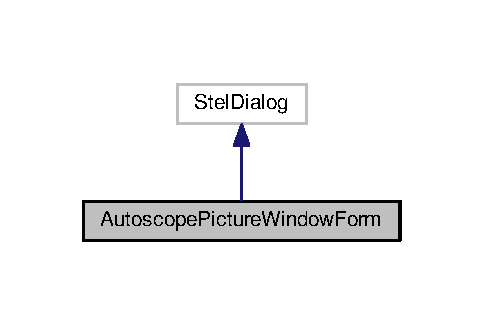
\includegraphics[width=232pt]{class_autoscope_picture_window_form__inherit__graph}
\end{center}
\end{figure}


Collaboration diagram for Autoscope\+Picture\+Window\+Form\+:
\nopagebreak
\begin{figure}[H]
\begin{center}
\leavevmode
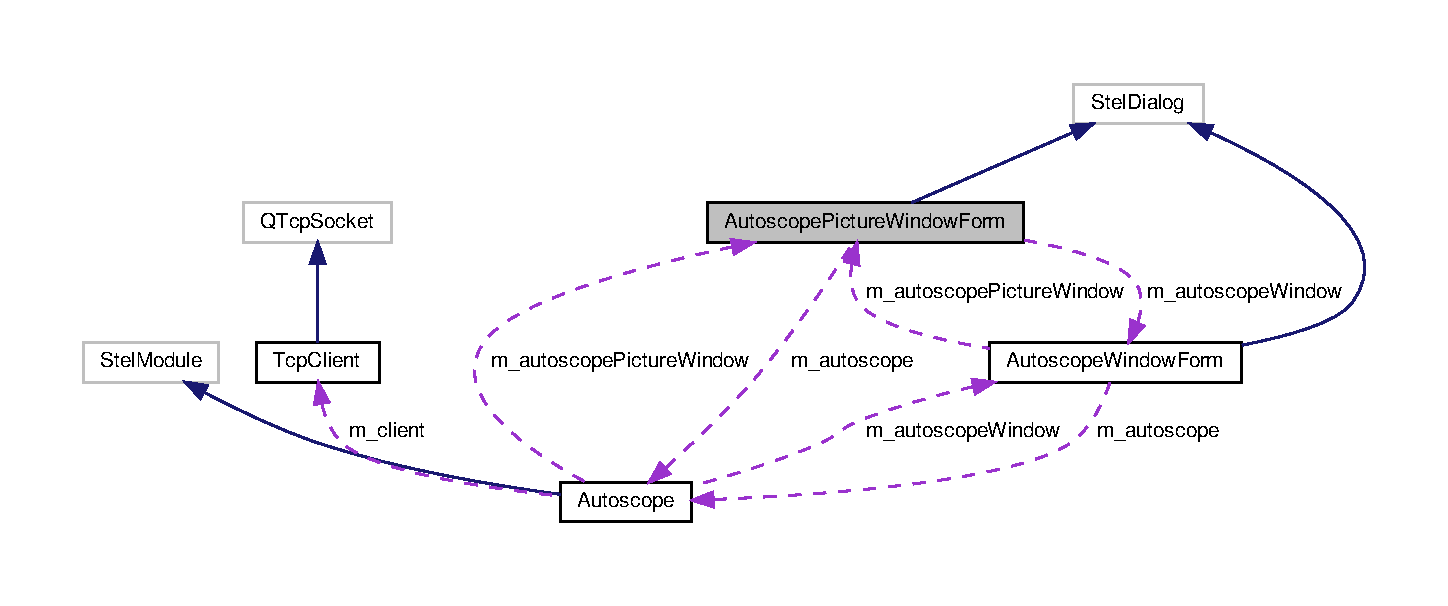
\includegraphics[width=350pt]{class_autoscope_picture_window_form__coll__graph}
\end{center}
\end{figure}
\subsection*{Public Slots}
\begin{DoxyCompactItemize}
\item 
void \mbox{\hyperlink{class_autoscope_picture_window_form_a4bcc43707d7b76b19d81ffc66a4b7ee2}{retranslate}} ()
\begin{DoxyCompactList}\small\item\em Inherited from the Stel\+Dialog class. \end{DoxyCompactList}\end{DoxyCompactItemize}
\subsection*{Public Member Functions}
\begin{DoxyCompactItemize}
\item 
\mbox{\hyperlink{class_autoscope_picture_window_form_ac7e1f8a94457cce24469119ea3214f8a}{Autoscope\+Picture\+Window\+Form}} ()
\begin{DoxyCompactList}\small\item\em Builder of the \mbox{\hyperlink{class_autoscope_picture_window_form}{Autoscope\+Picture\+Window\+Form}} class. \end{DoxyCompactList}\item 
\mbox{\hyperlink{class_autoscope_picture_window_form_a0ac8bae5bd9b170aea179812f0f516be}{$\sim$\+Autoscope\+Picture\+Window\+Form}} ()
\begin{DoxyCompactList}\small\item\em Destroyer of the \mbox{\hyperlink{class_autoscope_picture_window_form}{Autoscope\+Picture\+Window\+Form}} class. \end{DoxyCompactList}\item 
void \mbox{\hyperlink{class_autoscope_picture_window_form_a84ad64e4121c67a3269f935e50cfee2c}{update}} ()
\begin{DoxyCompactList}\small\item\em Method used to update calculation and displayed components. \end{DoxyCompactList}\item 
int \mbox{\hyperlink{class_autoscope_picture_window_form_ad9fa74865956b50029f0e2692ab256c8}{get\+Gui\+Horizontal\+Position}} (void)
\begin{DoxyCompactList}\small\item\em Getter used to retrieve the horizontal gui position. \end{DoxyCompactList}\item 
int \mbox{\hyperlink{class_autoscope_picture_window_form_ad7eeabfc680448ec5f663f7c68f6e3f4}{get\+Gui\+Vertical\+Position}} (void)
\begin{DoxyCompactList}\small\item\em Getter used to retrieve the vertical gui position. \end{DoxyCompactList}\item 
void \mbox{\hyperlink{class_autoscope_picture_window_form_a1a3b45dad146565be0f597e1b11cb910}{set\+Gui\+Horizontal\+Position}} (int)
\begin{DoxyCompactList}\small\item\em Setter used to set the horizontal gui position. \end{DoxyCompactList}\item 
void \mbox{\hyperlink{class_autoscope_picture_window_form_a687966c09f4fe03caa2b52c42a804ae1}{set\+Gui\+Vertical\+Position}} (int)
\begin{DoxyCompactList}\small\item\em Setter used to set the vertical gui position. \end{DoxyCompactList}\item 
int \mbox{\hyperlink{class_autoscope_picture_window_form_a7e8d04d5bf4eafc415a9d6176a2325e9}{get\+Gui\+Width}} (void)
\begin{DoxyCompactList}\small\item\em Getter used to retrieve the gui width. \end{DoxyCompactList}\item 
int \mbox{\hyperlink{class_autoscope_picture_window_form_ad3fa8efcfcc0631f8b646500fb5cea65}{get\+Gui\+Height}} (void)
\begin{DoxyCompactList}\small\item\em Getter used to retrieve the gui height. \end{DoxyCompactList}\item 
void \mbox{\hyperlink{class_autoscope_picture_window_form_ae968436e14e51184ca0f375f04947d4c}{set\+Gui\+Size}} (int)
\begin{DoxyCompactList}\small\item\em Setter used to set the gui size in percent of the screen. \end{DoxyCompactList}\item 
void \mbox{\hyperlink{class_autoscope_picture_window_form_a8c0ca53b5ca0a741cf240a0c07870bfe}{update\+Gui\+Size}} (void)
\begin{DoxyCompactList}\small\item\em Method used to update the size of the gui. \end{DoxyCompactList}\item 
void \mbox{\hyperlink{class_autoscope_picture_window_form_acb47c88be96f7b6573cd6181d6e3865e}{set\+Gui\+Opacity}} (double)
\begin{DoxyCompactList}\small\item\em Setter used to set the gui opacity. \end{DoxyCompactList}\item 
void \mbox{\hyperlink{class_autoscope_picture_window_form_aa9b0990a5e7fa9d0bedeaab959b999c6}{update\+Gui\+Position}} (void)
\begin{DoxyCompactList}\small\item\em Method used to update the gui position. \end{DoxyCompactList}\item 
void \mbox{\hyperlink{class_autoscope_picture_window_form_ac5673825fbee28ceaa21d962b92fbd42}{update\+Image}} (Q\+Pixmap image)
\begin{DoxyCompactList}\small\item\em Method used to update the image of the gui. \end{DoxyCompactList}\item 
void \mbox{\hyperlink{class_autoscope_picture_window_form_a14928e7fe4954367986932b7439fa132}{set\+Autoscope\+Window}} (\mbox{\hyperlink{class_autoscope_window_form}{Autoscope\+Window\+Form}} $\ast$autoscope\+Window)
\begin{DoxyCompactList}\small\item\em Setter used to initialize an instance of \mbox{\hyperlink{class_autoscope_window_form}{Autoscope\+Window\+Form}} class. \end{DoxyCompactList}\end{DoxyCompactItemize}
\subsection*{Protected Member Functions}
\begin{DoxyCompactItemize}
\item 
void \mbox{\hyperlink{class_autoscope_picture_window_form_a3014c48f6c7e48455f8908ca3f9acbbc}{create\+Dialog\+Content}} ()
\begin{DoxyCompactList}\small\item\em This method is inherited form the Stel\+Dialog class and is use to create the content of the dialog box. \end{DoxyCompactList}\end{DoxyCompactItemize}
\subsection*{Private Attributes}
\begin{DoxyCompactItemize}
\item 
Ui\+\_\+\+Autoscope\+Picture\+Window\+Form $\ast$ \mbox{\hyperlink{class_autoscope_picture_window_form_aac9815d1313c1814ff9f0eefa4eeb47d}{ui}}
\item 
\mbox{\hyperlink{class_autoscope}{Autoscope}} $\ast$ \mbox{\hyperlink{class_autoscope_picture_window_form_ab6166280899d69142f4d7ed787c63f8f}{m\+\_\+autoscope}}
\item 
\mbox{\hyperlink{class_autoscope_window_form}{Autoscope\+Window\+Form}} $\ast$ \mbox{\hyperlink{class_autoscope_picture_window_form_ae20e4b58eec25e79ec4a0b5b7fa10e21}{m\+\_\+autoscope\+Window}}
\item 
int \mbox{\hyperlink{class_autoscope_picture_window_form_aa5dacd6f9d13d4cafa98edae38d161f5}{m\+\_\+width}} = 192
\item 
int \mbox{\hyperlink{class_autoscope_picture_window_form_aba2d2633eaffee2cff0babc6db1ab1e4}{m\+\_\+height}} = 108
\item 
int \mbox{\hyperlink{class_autoscope_picture_window_form_a0bf8e1210cdea9fcf58b0153d52b7f6c}{m\+\_\+screen\+Width}}
\item 
int \mbox{\hyperlink{class_autoscope_picture_window_form_a760dd289327d7731dd40dd9f3543588a}{m\+\_\+screen\+Height}}
\item 
int \mbox{\hyperlink{class_autoscope_picture_window_form_ab85a9e8a721d8b8f9d50c03d7dd91eaf}{m\+\_\+gui\+Horizontal\+Position}} = 0
\item 
int \mbox{\hyperlink{class_autoscope_picture_window_form_acc65dba5ea960c1c8e38267b913a67d3}{m\+\_\+gui\+Vertical\+Position}} = 0
\end{DoxyCompactItemize}


\subsection{Detailed Description}
This class is use to build a picture display interface to show to the user the last taken picture. 

\subsection{Constructor \& Destructor Documentation}
\mbox{\Hypertarget{class_autoscope_picture_window_form_ac7e1f8a94457cce24469119ea3214f8a}\label{class_autoscope_picture_window_form_ac7e1f8a94457cce24469119ea3214f8a}} 
\index{AutoscopePictureWindowForm@{AutoscopePictureWindowForm}!AutoscopePictureWindowForm@{AutoscopePictureWindowForm}}
\index{AutoscopePictureWindowForm@{AutoscopePictureWindowForm}!AutoscopePictureWindowForm@{AutoscopePictureWindowForm}}
\subsubsection{\texorpdfstring{AutoscopePictureWindowForm()}{AutoscopePictureWindowForm()}}
{\footnotesize\ttfamily Autoscope\+Picture\+Window\+Form\+::\+Autoscope\+Picture\+Window\+Form (\begin{DoxyParamCaption}{ }\end{DoxyParamCaption})}



Builder of the \mbox{\hyperlink{class_autoscope_picture_window_form}{Autoscope\+Picture\+Window\+Form}} class. 

\mbox{\Hypertarget{class_autoscope_picture_window_form_a0ac8bae5bd9b170aea179812f0f516be}\label{class_autoscope_picture_window_form_a0ac8bae5bd9b170aea179812f0f516be}} 
\index{AutoscopePictureWindowForm@{AutoscopePictureWindowForm}!````~AutoscopePictureWindowForm@{$\sim$AutoscopePictureWindowForm}}
\index{````~AutoscopePictureWindowForm@{$\sim$AutoscopePictureWindowForm}!AutoscopePictureWindowForm@{AutoscopePictureWindowForm}}
\subsubsection{\texorpdfstring{$\sim$AutoscopePictureWindowForm()}{~AutoscopePictureWindowForm()}}
{\footnotesize\ttfamily Autoscope\+Picture\+Window\+Form\+::$\sim$\+Autoscope\+Picture\+Window\+Form (\begin{DoxyParamCaption}{ }\end{DoxyParamCaption})}



Destroyer of the \mbox{\hyperlink{class_autoscope_picture_window_form}{Autoscope\+Picture\+Window\+Form}} class. 



\subsection{Member Function Documentation}
\mbox{\Hypertarget{class_autoscope_picture_window_form_a3014c48f6c7e48455f8908ca3f9acbbc}\label{class_autoscope_picture_window_form_a3014c48f6c7e48455f8908ca3f9acbbc}} 
\index{AutoscopePictureWindowForm@{AutoscopePictureWindowForm}!createDialogContent@{createDialogContent}}
\index{createDialogContent@{createDialogContent}!AutoscopePictureWindowForm@{AutoscopePictureWindowForm}}
\subsubsection{\texorpdfstring{createDialogContent()}{createDialogContent()}}
{\footnotesize\ttfamily void Autoscope\+Picture\+Window\+Form\+::create\+Dialog\+Content (\begin{DoxyParamCaption}{ }\end{DoxyParamCaption})\hspace{0.3cm}{\ttfamily [protected]}}



This method is inherited form the Stel\+Dialog class and is use to create the content of the dialog box. 

\begin{DoxySeeAlso}{See also}
Stel\+Dialog 
\end{DoxySeeAlso}
\mbox{\Hypertarget{class_autoscope_picture_window_form_ad3fa8efcfcc0631f8b646500fb5cea65}\label{class_autoscope_picture_window_form_ad3fa8efcfcc0631f8b646500fb5cea65}} 
\index{AutoscopePictureWindowForm@{AutoscopePictureWindowForm}!getGuiHeight@{getGuiHeight}}
\index{getGuiHeight@{getGuiHeight}!AutoscopePictureWindowForm@{AutoscopePictureWindowForm}}
\subsubsection{\texorpdfstring{getGuiHeight()}{getGuiHeight()}}
{\footnotesize\ttfamily int Autoscope\+Picture\+Window\+Form\+::get\+Gui\+Height (\begin{DoxyParamCaption}\item[{void}]{ }\end{DoxyParamCaption})}



Getter used to retrieve the gui height. 

\begin{DoxyReturn}{Returns}
The gui height 
\end{DoxyReturn}
\mbox{\Hypertarget{class_autoscope_picture_window_form_ad9fa74865956b50029f0e2692ab256c8}\label{class_autoscope_picture_window_form_ad9fa74865956b50029f0e2692ab256c8}} 
\index{AutoscopePictureWindowForm@{AutoscopePictureWindowForm}!getGuiHorizontalPosition@{getGuiHorizontalPosition}}
\index{getGuiHorizontalPosition@{getGuiHorizontalPosition}!AutoscopePictureWindowForm@{AutoscopePictureWindowForm}}
\subsubsection{\texorpdfstring{getGuiHorizontalPosition()}{getGuiHorizontalPosition()}}
{\footnotesize\ttfamily int Autoscope\+Picture\+Window\+Form\+::get\+Gui\+Horizontal\+Position (\begin{DoxyParamCaption}\item[{void}]{ }\end{DoxyParamCaption})}



Getter used to retrieve the horizontal gui position. 

\begin{DoxyReturn}{Returns}
The horizontal gui position 
\end{DoxyReturn}
\mbox{\Hypertarget{class_autoscope_picture_window_form_ad7eeabfc680448ec5f663f7c68f6e3f4}\label{class_autoscope_picture_window_form_ad7eeabfc680448ec5f663f7c68f6e3f4}} 
\index{AutoscopePictureWindowForm@{AutoscopePictureWindowForm}!getGuiVerticalPosition@{getGuiVerticalPosition}}
\index{getGuiVerticalPosition@{getGuiVerticalPosition}!AutoscopePictureWindowForm@{AutoscopePictureWindowForm}}
\subsubsection{\texorpdfstring{getGuiVerticalPosition()}{getGuiVerticalPosition()}}
{\footnotesize\ttfamily int Autoscope\+Picture\+Window\+Form\+::get\+Gui\+Vertical\+Position (\begin{DoxyParamCaption}\item[{void}]{ }\end{DoxyParamCaption})}



Getter used to retrieve the vertical gui position. 

\begin{DoxyReturn}{Returns}
The vertical gui position 
\end{DoxyReturn}
\mbox{\Hypertarget{class_autoscope_picture_window_form_a7e8d04d5bf4eafc415a9d6176a2325e9}\label{class_autoscope_picture_window_form_a7e8d04d5bf4eafc415a9d6176a2325e9}} 
\index{AutoscopePictureWindowForm@{AutoscopePictureWindowForm}!getGuiWidth@{getGuiWidth}}
\index{getGuiWidth@{getGuiWidth}!AutoscopePictureWindowForm@{AutoscopePictureWindowForm}}
\subsubsection{\texorpdfstring{getGuiWidth()}{getGuiWidth()}}
{\footnotesize\ttfamily int Autoscope\+Picture\+Window\+Form\+::get\+Gui\+Width (\begin{DoxyParamCaption}\item[{void}]{ }\end{DoxyParamCaption})}



Getter used to retrieve the gui width. 

\begin{DoxyReturn}{Returns}
The gui width 
\end{DoxyReturn}
\mbox{\Hypertarget{class_autoscope_picture_window_form_a4bcc43707d7b76b19d81ffc66a4b7ee2}\label{class_autoscope_picture_window_form_a4bcc43707d7b76b19d81ffc66a4b7ee2}} 
\index{AutoscopePictureWindowForm@{AutoscopePictureWindowForm}!retranslate@{retranslate}}
\index{retranslate@{retranslate}!AutoscopePictureWindowForm@{AutoscopePictureWindowForm}}
\subsubsection{\texorpdfstring{retranslate}{retranslate}}
{\footnotesize\ttfamily void Autoscope\+Picture\+Window\+Form\+::retranslate (\begin{DoxyParamCaption}{ }\end{DoxyParamCaption})\hspace{0.3cm}{\ttfamily [slot]}}



Inherited from the Stel\+Dialog class. 

\begin{DoxySeeAlso}{See also}
Stel\+Dialog 
\end{DoxySeeAlso}
\mbox{\Hypertarget{class_autoscope_picture_window_form_a14928e7fe4954367986932b7439fa132}\label{class_autoscope_picture_window_form_a14928e7fe4954367986932b7439fa132}} 
\index{AutoscopePictureWindowForm@{AutoscopePictureWindowForm}!setAutoscopeWindow@{setAutoscopeWindow}}
\index{setAutoscopeWindow@{setAutoscopeWindow}!AutoscopePictureWindowForm@{AutoscopePictureWindowForm}}
\subsubsection{\texorpdfstring{setAutoscopeWindow()}{setAutoscopeWindow()}}
{\footnotesize\ttfamily void Autoscope\+Picture\+Window\+Form\+::set\+Autoscope\+Window (\begin{DoxyParamCaption}\item[{\mbox{\hyperlink{class_autoscope_window_form}{Autoscope\+Window\+Form}} $\ast$}]{autoscope\+Window }\end{DoxyParamCaption})\hspace{0.3cm}{\ttfamily [inline]}}



Setter used to initialize an instance of \mbox{\hyperlink{class_autoscope_window_form}{Autoscope\+Window\+Form}} class. 


\begin{DoxyParams}{Parameters}
{\em autoscope\+Window} & an instance of \mbox{\hyperlink{class_autoscope_window_form}{Autoscope\+Window\+Form}} class \\
\hline
\end{DoxyParams}
\mbox{\Hypertarget{class_autoscope_picture_window_form_a1a3b45dad146565be0f597e1b11cb910}\label{class_autoscope_picture_window_form_a1a3b45dad146565be0f597e1b11cb910}} 
\index{AutoscopePictureWindowForm@{AutoscopePictureWindowForm}!setGuiHorizontalPosition@{setGuiHorizontalPosition}}
\index{setGuiHorizontalPosition@{setGuiHorizontalPosition}!AutoscopePictureWindowForm@{AutoscopePictureWindowForm}}
\subsubsection{\texorpdfstring{setGuiHorizontalPosition()}{setGuiHorizontalPosition()}}
{\footnotesize\ttfamily void Autoscope\+Picture\+Window\+Form\+::set\+Gui\+Horizontal\+Position (\begin{DoxyParamCaption}\item[{int}]{i }\end{DoxyParamCaption})}



Setter used to set the horizontal gui position. 


\begin{DoxyParams}{Parameters}
{\em The} & horizontal gui position in pixel \\
\hline
\end{DoxyParams}
\mbox{\Hypertarget{class_autoscope_picture_window_form_acb47c88be96f7b6573cd6181d6e3865e}\label{class_autoscope_picture_window_form_acb47c88be96f7b6573cd6181d6e3865e}} 
\index{AutoscopePictureWindowForm@{AutoscopePictureWindowForm}!setGuiOpacity@{setGuiOpacity}}
\index{setGuiOpacity@{setGuiOpacity}!AutoscopePictureWindowForm@{AutoscopePictureWindowForm}}
\subsubsection{\texorpdfstring{setGuiOpacity()}{setGuiOpacity()}}
{\footnotesize\ttfamily void Autoscope\+Picture\+Window\+Form\+::set\+Gui\+Opacity (\begin{DoxyParamCaption}\item[{double}]{opacity }\end{DoxyParamCaption})}



Setter used to set the gui opacity. 


\begin{DoxyParams}{Parameters}
{\em the} & gui opacity \\
\hline
\end{DoxyParams}
\mbox{\Hypertarget{class_autoscope_picture_window_form_ae968436e14e51184ca0f375f04947d4c}\label{class_autoscope_picture_window_form_ae968436e14e51184ca0f375f04947d4c}} 
\index{AutoscopePictureWindowForm@{AutoscopePictureWindowForm}!setGuiSize@{setGuiSize}}
\index{setGuiSize@{setGuiSize}!AutoscopePictureWindowForm@{AutoscopePictureWindowForm}}
\subsubsection{\texorpdfstring{setGuiSize()}{setGuiSize()}}
{\footnotesize\ttfamily void Autoscope\+Picture\+Window\+Form\+::set\+Gui\+Size (\begin{DoxyParamCaption}\item[{int}]{percent }\end{DoxyParamCaption})}



Setter used to set the gui size in percent of the screen. 


\begin{DoxyParams}{Parameters}
{\em The} & gui size in percent of the screen \\
\hline
\end{DoxyParams}
\mbox{\Hypertarget{class_autoscope_picture_window_form_a687966c09f4fe03caa2b52c42a804ae1}\label{class_autoscope_picture_window_form_a687966c09f4fe03caa2b52c42a804ae1}} 
\index{AutoscopePictureWindowForm@{AutoscopePictureWindowForm}!setGuiVerticalPosition@{setGuiVerticalPosition}}
\index{setGuiVerticalPosition@{setGuiVerticalPosition}!AutoscopePictureWindowForm@{AutoscopePictureWindowForm}}
\subsubsection{\texorpdfstring{setGuiVerticalPosition()}{setGuiVerticalPosition()}}
{\footnotesize\ttfamily void Autoscope\+Picture\+Window\+Form\+::set\+Gui\+Vertical\+Position (\begin{DoxyParamCaption}\item[{int}]{i }\end{DoxyParamCaption})}



Setter used to set the vertical gui position. 


\begin{DoxyParams}{Parameters}
{\em The} & vertical gui position in pixel \\
\hline
\end{DoxyParams}
\mbox{\Hypertarget{class_autoscope_picture_window_form_a84ad64e4121c67a3269f935e50cfee2c}\label{class_autoscope_picture_window_form_a84ad64e4121c67a3269f935e50cfee2c}} 
\index{AutoscopePictureWindowForm@{AutoscopePictureWindowForm}!update@{update}}
\index{update@{update}!AutoscopePictureWindowForm@{AutoscopePictureWindowForm}}
\subsubsection{\texorpdfstring{update()}{update()}}
{\footnotesize\ttfamily void Autoscope\+Picture\+Window\+Form\+::update (\begin{DoxyParamCaption}{ }\end{DoxyParamCaption})}



Method used to update calculation and displayed components. 

\mbox{\Hypertarget{class_autoscope_picture_window_form_aa9b0990a5e7fa9d0bedeaab959b999c6}\label{class_autoscope_picture_window_form_aa9b0990a5e7fa9d0bedeaab959b999c6}} 
\index{AutoscopePictureWindowForm@{AutoscopePictureWindowForm}!updateGuiPosition@{updateGuiPosition}}
\index{updateGuiPosition@{updateGuiPosition}!AutoscopePictureWindowForm@{AutoscopePictureWindowForm}}
\subsubsection{\texorpdfstring{updateGuiPosition()}{updateGuiPosition()}}
{\footnotesize\ttfamily void Autoscope\+Picture\+Window\+Form\+::update\+Gui\+Position (\begin{DoxyParamCaption}\item[{void}]{ }\end{DoxyParamCaption})}



Method used to update the gui position. 

\mbox{\Hypertarget{class_autoscope_picture_window_form_a8c0ca53b5ca0a741cf240a0c07870bfe}\label{class_autoscope_picture_window_form_a8c0ca53b5ca0a741cf240a0c07870bfe}} 
\index{AutoscopePictureWindowForm@{AutoscopePictureWindowForm}!updateGuiSize@{updateGuiSize}}
\index{updateGuiSize@{updateGuiSize}!AutoscopePictureWindowForm@{AutoscopePictureWindowForm}}
\subsubsection{\texorpdfstring{updateGuiSize()}{updateGuiSize()}}
{\footnotesize\ttfamily void Autoscope\+Picture\+Window\+Form\+::update\+Gui\+Size (\begin{DoxyParamCaption}\item[{void}]{ }\end{DoxyParamCaption})}



Method used to update the size of the gui. 

\mbox{\Hypertarget{class_autoscope_picture_window_form_ac5673825fbee28ceaa21d962b92fbd42}\label{class_autoscope_picture_window_form_ac5673825fbee28ceaa21d962b92fbd42}} 
\index{AutoscopePictureWindowForm@{AutoscopePictureWindowForm}!updateImage@{updateImage}}
\index{updateImage@{updateImage}!AutoscopePictureWindowForm@{AutoscopePictureWindowForm}}
\subsubsection{\texorpdfstring{updateImage()}{updateImage()}}
{\footnotesize\ttfamily void Autoscope\+Picture\+Window\+Form\+::update\+Image (\begin{DoxyParamCaption}\item[{Q\+Pixmap}]{image }\end{DoxyParamCaption})}



Method used to update the image of the gui. 


\begin{DoxyParams}{Parameters}
{\em image} & \\
\hline
\end{DoxyParams}


\subsection{Member Data Documentation}
\mbox{\Hypertarget{class_autoscope_picture_window_form_ab6166280899d69142f4d7ed787c63f8f}\label{class_autoscope_picture_window_form_ab6166280899d69142f4d7ed787c63f8f}} 
\index{AutoscopePictureWindowForm@{AutoscopePictureWindowForm}!m\_autoscope@{m\_autoscope}}
\index{m\_autoscope@{m\_autoscope}!AutoscopePictureWindowForm@{AutoscopePictureWindowForm}}
\subsubsection{\texorpdfstring{m\_autoscope}{m\_autoscope}}
{\footnotesize\ttfamily \mbox{\hyperlink{class_autoscope}{Autoscope}}$\ast$ Autoscope\+Picture\+Window\+Form\+::m\+\_\+autoscope\hspace{0.3cm}{\ttfamily [private]}}

An instance of the \mbox{\hyperlink{class_autoscope}{Autoscope}} class \mbox{\Hypertarget{class_autoscope_picture_window_form_ae20e4b58eec25e79ec4a0b5b7fa10e21}\label{class_autoscope_picture_window_form_ae20e4b58eec25e79ec4a0b5b7fa10e21}} 
\index{AutoscopePictureWindowForm@{AutoscopePictureWindowForm}!m\_autoscopeWindow@{m\_autoscopeWindow}}
\index{m\_autoscopeWindow@{m\_autoscopeWindow}!AutoscopePictureWindowForm@{AutoscopePictureWindowForm}}
\subsubsection{\texorpdfstring{m\_autoscopeWindow}{m\_autoscopeWindow}}
{\footnotesize\ttfamily \mbox{\hyperlink{class_autoscope_window_form}{Autoscope\+Window\+Form}}$\ast$ Autoscope\+Picture\+Window\+Form\+::m\+\_\+autoscope\+Window\hspace{0.3cm}{\ttfamily [private]}}

An instance of the \mbox{\hyperlink{class_autoscope_window_form}{Autoscope\+Window\+Form}} class \mbox{\Hypertarget{class_autoscope_picture_window_form_ab85a9e8a721d8b8f9d50c03d7dd91eaf}\label{class_autoscope_picture_window_form_ab85a9e8a721d8b8f9d50c03d7dd91eaf}} 
\index{AutoscopePictureWindowForm@{AutoscopePictureWindowForm}!m\_guiHorizontalPosition@{m\_guiHorizontalPosition}}
\index{m\_guiHorizontalPosition@{m\_guiHorizontalPosition}!AutoscopePictureWindowForm@{AutoscopePictureWindowForm}}
\subsubsection{\texorpdfstring{m\_guiHorizontalPosition}{m\_guiHorizontalPosition}}
{\footnotesize\ttfamily int Autoscope\+Picture\+Window\+Form\+::m\+\_\+gui\+Horizontal\+Position = 0\hspace{0.3cm}{\ttfamily [private]}}

The horizontal position of the dialog box \mbox{\Hypertarget{class_autoscope_picture_window_form_acc65dba5ea960c1c8e38267b913a67d3}\label{class_autoscope_picture_window_form_acc65dba5ea960c1c8e38267b913a67d3}} 
\index{AutoscopePictureWindowForm@{AutoscopePictureWindowForm}!m\_guiVerticalPosition@{m\_guiVerticalPosition}}
\index{m\_guiVerticalPosition@{m\_guiVerticalPosition}!AutoscopePictureWindowForm@{AutoscopePictureWindowForm}}
\subsubsection{\texorpdfstring{m\_guiVerticalPosition}{m\_guiVerticalPosition}}
{\footnotesize\ttfamily int Autoscope\+Picture\+Window\+Form\+::m\+\_\+gui\+Vertical\+Position = 0\hspace{0.3cm}{\ttfamily [private]}}

The vertical position of the dialog box \mbox{\Hypertarget{class_autoscope_picture_window_form_aba2d2633eaffee2cff0babc6db1ab1e4}\label{class_autoscope_picture_window_form_aba2d2633eaffee2cff0babc6db1ab1e4}} 
\index{AutoscopePictureWindowForm@{AutoscopePictureWindowForm}!m\_height@{m\_height}}
\index{m\_height@{m\_height}!AutoscopePictureWindowForm@{AutoscopePictureWindowForm}}
\subsubsection{\texorpdfstring{m\_height}{m\_height}}
{\footnotesize\ttfamily int Autoscope\+Picture\+Window\+Form\+::m\+\_\+height = 108\hspace{0.3cm}{\ttfamily [private]}}

The height of the dialog box \mbox{\Hypertarget{class_autoscope_picture_window_form_a760dd289327d7731dd40dd9f3543588a}\label{class_autoscope_picture_window_form_a760dd289327d7731dd40dd9f3543588a}} 
\index{AutoscopePictureWindowForm@{AutoscopePictureWindowForm}!m\_screenHeight@{m\_screenHeight}}
\index{m\_screenHeight@{m\_screenHeight}!AutoscopePictureWindowForm@{AutoscopePictureWindowForm}}
\subsubsection{\texorpdfstring{m\_screenHeight}{m\_screenHeight}}
{\footnotesize\ttfamily int Autoscope\+Picture\+Window\+Form\+::m\+\_\+screen\+Height\hspace{0.3cm}{\ttfamily [private]}}

The height of the screen \mbox{\Hypertarget{class_autoscope_picture_window_form_a0bf8e1210cdea9fcf58b0153d52b7f6c}\label{class_autoscope_picture_window_form_a0bf8e1210cdea9fcf58b0153d52b7f6c}} 
\index{AutoscopePictureWindowForm@{AutoscopePictureWindowForm}!m\_screenWidth@{m\_screenWidth}}
\index{m\_screenWidth@{m\_screenWidth}!AutoscopePictureWindowForm@{AutoscopePictureWindowForm}}
\subsubsection{\texorpdfstring{m\_screenWidth}{m\_screenWidth}}
{\footnotesize\ttfamily int Autoscope\+Picture\+Window\+Form\+::m\+\_\+screen\+Width\hspace{0.3cm}{\ttfamily [private]}}

The width of the screen \mbox{\Hypertarget{class_autoscope_picture_window_form_aa5dacd6f9d13d4cafa98edae38d161f5}\label{class_autoscope_picture_window_form_aa5dacd6f9d13d4cafa98edae38d161f5}} 
\index{AutoscopePictureWindowForm@{AutoscopePictureWindowForm}!m\_width@{m\_width}}
\index{m\_width@{m\_width}!AutoscopePictureWindowForm@{AutoscopePictureWindowForm}}
\subsubsection{\texorpdfstring{m\_width}{m\_width}}
{\footnotesize\ttfamily int Autoscope\+Picture\+Window\+Form\+::m\+\_\+width = 192\hspace{0.3cm}{\ttfamily [private]}}

The width of the dialog box \mbox{\Hypertarget{class_autoscope_picture_window_form_aac9815d1313c1814ff9f0eefa4eeb47d}\label{class_autoscope_picture_window_form_aac9815d1313c1814ff9f0eefa4eeb47d}} 
\index{AutoscopePictureWindowForm@{AutoscopePictureWindowForm}!ui@{ui}}
\index{ui@{ui}!AutoscopePictureWindowForm@{AutoscopePictureWindowForm}}
\subsubsection{\texorpdfstring{ui}{ui}}
{\footnotesize\ttfamily Ui\+\_\+\+Autoscope\+Picture\+Window\+Form$\ast$ Autoscope\+Picture\+Window\+Form\+::ui\hspace{0.3cm}{\ttfamily [private]}}

An instance of the Ui\+\_\+\+Autoscope\+Picture\+Window\+Form class 

The documentation for this class was generated from the following files\+:\begin{DoxyCompactItemize}
\item 
src/gui/\mbox{\hyperlink{_autoscope_picture_window_form_8hpp}{Autoscope\+Picture\+Window\+Form.\+hpp}}\item 
src/gui/\mbox{\hyperlink{_autoscope_picture_window_form_8cpp}{Autoscope\+Picture\+Window\+Form.\+cpp}}\end{DoxyCompactItemize}

\hypertarget{class_autoscope_stel_plugin_interface}{}\section{Autoscope\+Stel\+Plugin\+Interface Class Reference}
\label{class_autoscope_stel_plugin_interface}\index{Autoscope\+Stel\+Plugin\+Interface@{Autoscope\+Stel\+Plugin\+Interface}}


This class is used by Qt to manage a plug-\/in interface.  




{\ttfamily \#include $<$Autoscope.\+hpp$>$}



Inheritance diagram for Autoscope\+Stel\+Plugin\+Interface\+:
\nopagebreak
\begin{figure}[H]
\begin{center}
\leavevmode
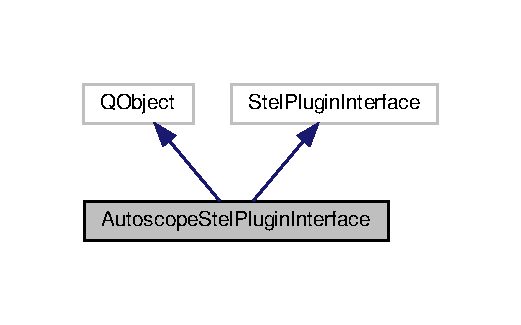
\includegraphics[width=250pt]{class_autoscope_stel_plugin_interface__inherit__graph}
\end{center}
\end{figure}


Collaboration diagram for Autoscope\+Stel\+Plugin\+Interface\+:
\nopagebreak
\begin{figure}[H]
\begin{center}
\leavevmode
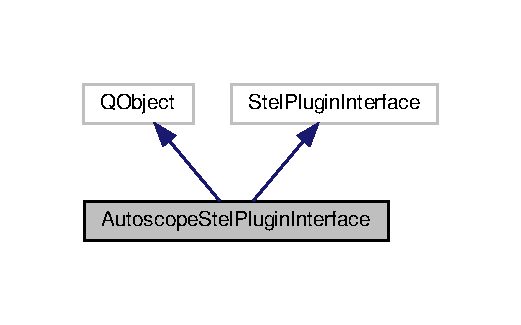
\includegraphics[width=250pt]{class_autoscope_stel_plugin_interface__coll__graph}
\end{center}
\end{figure}
\subsection*{Public Member Functions}
\begin{DoxyCompactItemize}
\item 
virtual Stel\+Module $\ast$ \hyperlink{class_autoscope_stel_plugin_interface_a8cd35ee4a5e37defb00ebbc6cade99ad}{get\+Stel\+Module} () const 
\item 
virtual Stel\+Plugin\+Info \hyperlink{class_autoscope_stel_plugin_interface_a64870294f54ab21f331903d01558a632}{get\+Plugin\+Info} () const 
\item 
virtual Q\+Object\+List \hyperlink{class_autoscope_stel_plugin_interface_a4698450c65637c6a2005ce6aaba6fed7}{get\+Extension\+List} () const 
\end{DoxyCompactItemize}


\subsection{Detailed Description}
This class is used by Qt to manage a plug-\/in interface. 

\subsection{Member Function Documentation}
\index{Autoscope\+Stel\+Plugin\+Interface@{Autoscope\+Stel\+Plugin\+Interface}!get\+Extension\+List@{get\+Extension\+List}}
\index{get\+Extension\+List@{get\+Extension\+List}!Autoscope\+Stel\+Plugin\+Interface@{Autoscope\+Stel\+Plugin\+Interface}}
\subsubsection[{\texorpdfstring{get\+Extension\+List() const }{getExtensionList() const }}]{\setlength{\rightskip}{0pt plus 5cm}virtual Q\+Object\+List Autoscope\+Stel\+Plugin\+Interface\+::get\+Extension\+List (
\begin{DoxyParamCaption}
{}
\end{DoxyParamCaption}
) const\hspace{0.3cm}{\ttfamily [inline]}, {\ttfamily [virtual]}}\hypertarget{class_autoscope_stel_plugin_interface_a4698450c65637c6a2005ce6aaba6fed7}{}\label{class_autoscope_stel_plugin_interface_a4698450c65637c6a2005ce6aaba6fed7}
\index{Autoscope\+Stel\+Plugin\+Interface@{Autoscope\+Stel\+Plugin\+Interface}!get\+Plugin\+Info@{get\+Plugin\+Info}}
\index{get\+Plugin\+Info@{get\+Plugin\+Info}!Autoscope\+Stel\+Plugin\+Interface@{Autoscope\+Stel\+Plugin\+Interface}}
\subsubsection[{\texorpdfstring{get\+Plugin\+Info() const }{getPluginInfo() const }}]{\setlength{\rightskip}{0pt plus 5cm}Stel\+Plugin\+Info Autoscope\+Stel\+Plugin\+Interface\+::get\+Plugin\+Info (
\begin{DoxyParamCaption}
{}
\end{DoxyParamCaption}
) const\hspace{0.3cm}{\ttfamily [virtual]}}\hypertarget{class_autoscope_stel_plugin_interface_a64870294f54ab21f331903d01558a632}{}\label{class_autoscope_stel_plugin_interface_a64870294f54ab21f331903d01558a632}
\index{Autoscope\+Stel\+Plugin\+Interface@{Autoscope\+Stel\+Plugin\+Interface}!get\+Stel\+Module@{get\+Stel\+Module}}
\index{get\+Stel\+Module@{get\+Stel\+Module}!Autoscope\+Stel\+Plugin\+Interface@{Autoscope\+Stel\+Plugin\+Interface}}
\subsubsection[{\texorpdfstring{get\+Stel\+Module() const }{getStelModule() const }}]{\setlength{\rightskip}{0pt plus 5cm}Stel\+Module $\ast$ Autoscope\+Stel\+Plugin\+Interface\+::get\+Stel\+Module (
\begin{DoxyParamCaption}
{}
\end{DoxyParamCaption}
) const\hspace{0.3cm}{\ttfamily [virtual]}}\hypertarget{class_autoscope_stel_plugin_interface_a8cd35ee4a5e37defb00ebbc6cade99ad}{}\label{class_autoscope_stel_plugin_interface_a8cd35ee4a5e37defb00ebbc6cade99ad}


The documentation for this class was generated from the following files\+:\begin{DoxyCompactItemize}
\item 
src/\hyperlink{_autoscope_8hpp}{Autoscope.\+hpp}\item 
src/\hyperlink{_autoscope_8cpp}{Autoscope.\+cpp}\end{DoxyCompactItemize}

\hypertarget{class_autoscope_window_form}{}\section{Autoscope\+Window\+Form Class Reference}
\label{class_autoscope_window_form}\index{Autoscope\+Window\+Form@{Autoscope\+Window\+Form}}


This class is use to build a configuration interface between the user and the plugin.  




{\ttfamily \#include $<$Autoscope\+Window\+Form.\+hpp$>$}



Inheritance diagram for Autoscope\+Window\+Form\+:
\nopagebreak
\begin{figure}[H]
\begin{center}
\leavevmode
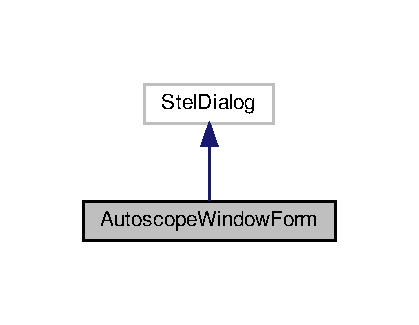
\includegraphics[width=201pt]{class_autoscope_window_form__inherit__graph}
\end{center}
\end{figure}


Collaboration diagram for Autoscope\+Window\+Form\+:
\nopagebreak
\begin{figure}[H]
\begin{center}
\leavevmode
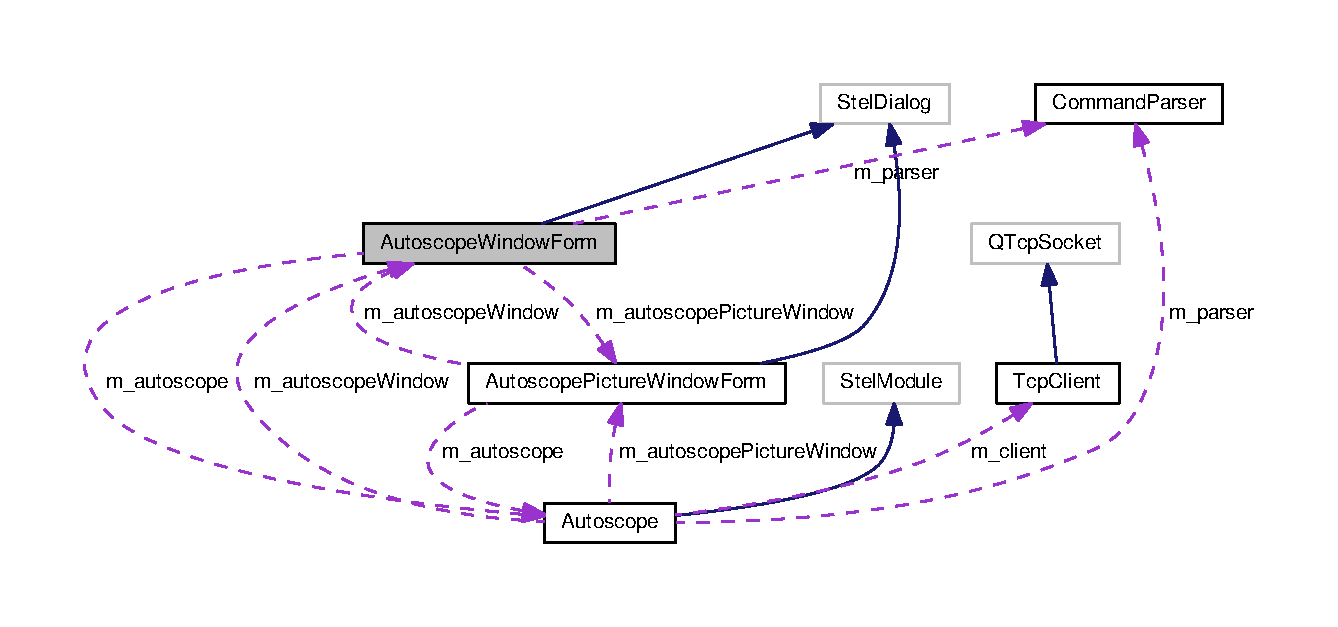
\includegraphics[width=350pt]{class_autoscope_window_form__coll__graph}
\end{center}
\end{figure}
\subsection*{Public Slots}
\begin{DoxyCompactItemize}
\item 
void \hyperlink{class_autoscope_window_form_a3f3d731c45d104fee58dd4c2dcc6fd86}{retranslate} ()
\begin{DoxyCompactList}\small\item\em Inherited from the Stel\+Dialog class. \end{DoxyCompactList}\item 
void \hyperlink{class_autoscope_window_form_ac6b0a28c17efb188b234ce1c08baa82d}{start\+Button\+Pressed} (void)
\begin{DoxyCompactList}\small\item\em Start initialization of the telescope. \end{DoxyCompactList}\item 
void \hyperlink{class_autoscope_window_form_ad7b04807a37c5014ab3a151d2ce720b7}{track\+Button\+Pressed} (void)
\begin{DoxyCompactList}\small\item\em Start tracking the selected object. \end{DoxyCompactList}\item 
void \hyperlink{class_autoscope_window_form_a867b2e9355138f8b41c17dba563c43ef}{untrack\+Button\+Pressed} (void)
\begin{DoxyCompactList}\small\item\em Stop tracking the tracked object. \end{DoxyCompactList}\item 
void \hyperlink{class_autoscope_window_form_ac78048dc833bd4952108cb5fe8cac6f8}{take\+Picture\+Button\+Pressed} (void)
\begin{DoxyCompactList}\small\item\em Send a command to the telescope to take a picture. \end{DoxyCompactList}\item 
void \hyperlink{class_autoscope_window_form_ae7caa21b226f06d2f32fd6da6d539bbf}{toggle\+Display\+Button\+Pressed} (void)
\begin{DoxyCompactList}\small\item\em Toggle the visibility of the picture display. \end{DoxyCompactList}\end{DoxyCompactItemize}
\subsection*{Public Member Functions}
\begin{DoxyCompactItemize}
\item 
\hyperlink{class_autoscope_window_form_abff392139c212a6f9e183d3984a02a47}{Autoscope\+Window\+Form} ()
\begin{DoxyCompactList}\small\item\em Builder of the \hyperlink{class_autoscope_window_form}{Autoscope\+Window\+Form} class. \end{DoxyCompactList}\item 
\hyperlink{class_autoscope_window_form_a2a7cceef655815a6c6ee1cc65a40fa8d}{$\sim$\+Autoscope\+Window\+Form} ()
\begin{DoxyCompactList}\small\item\em Destroyer of the \hyperlink{class_autoscope_window_form}{Autoscope\+Window\+Form} class. \end{DoxyCompactList}\item 
void \hyperlink{class_autoscope_window_form_a732f751b8de766e03f5f79a7a08db136}{update} ()
\begin{DoxyCompactList}\small\item\em Method used to update calculation and displayed components. \end{DoxyCompactList}\item 
void \hyperlink{class_autoscope_window_form_a4308f566557feaba98e031e28e527812}{set\+Autoscope\+Picture\+Window} (\hyperlink{class_autoscope_picture_window_form}{Autoscope\+Picture\+Window\+Form} $\ast$autoscope\+Picture\+Window)
\begin{DoxyCompactList}\small\item\em Setter used to initialize an instance of \hyperlink{class_autoscope_picture_window_form}{Autoscope\+Picture\+Window\+Form} class. \end{DoxyCompactList}\item 
int \hyperlink{class_autoscope_window_form_ad065e4a2a518d779407238e3c258f6e6}{get\+Gui\+Horizontal\+Position} (void)
\begin{DoxyCompactList}\small\item\em Getter used to retrieve the horizontal gui position. \end{DoxyCompactList}\item 
int \hyperlink{class_autoscope_window_form_a0d92cd0c7342749009e12058517ba060}{get\+Gui\+Vertical\+Position} (void)
\begin{DoxyCompactList}\small\item\em Getter used to retrieve the vertical gui position. \end{DoxyCompactList}\item 
int \hyperlink{class_autoscope_window_form_a51b6c47d99b53207d9e65157f01270ff}{get\+Screen\+Size\+Percent} (void)
\begin{DoxyCompactList}\small\item\em Getter used to retrieve the value of the display size editor. \end{DoxyCompactList}\item 
void \hyperlink{class_autoscope_window_form_af62e38bc2170d8504f63f07e5d0b4943}{update\+Gui\+Size} (void)
\begin{DoxyCompactList}\small\item\em Method used to update the gui size. \end{DoxyCompactList}\item 
void \hyperlink{class_autoscope_window_form_aada2c3ef979ce1718bb981490f6c7495}{update\+Gui\+Position} (void)
\begin{DoxyCompactList}\small\item\em Method used to update the gui position. \end{DoxyCompactList}\item 
void \hyperlink{class_autoscope_window_form_adfa249163e1c2a72485c24a575a67efb}{toggle\+Display} (void)
\begin{DoxyCompactList}\small\item\em Method used to toggle the visibility of the picture display. \end{DoxyCompactList}\item 
void \hyperlink{class_autoscope_window_form_a38a4a73945cffab764db46b8deec800a}{update\+Ip\+Messenger\+Text} (Q\+String)
\begin{DoxyCompactList}\small\item\em Method used to update the IP messenger text. \end{DoxyCompactList}\end{DoxyCompactItemize}
\subsection*{Protected Member Functions}
\begin{DoxyCompactItemize}
\item 
void \hyperlink{class_autoscope_window_form_ab48246f0892a43963b7d209dc3bf4b4f}{create\+Dialog\+Content} ()
\begin{DoxyCompactList}\small\item\em This method is inherited form the Stel\+Dialog class and it\textquotesingle{}s use to create the content of the dialog box. \end{DoxyCompactList}\end{DoxyCompactItemize}
\subsection*{Private Slots}
\begin{DoxyCompactItemize}
\item 
void \hyperlink{class_autoscope_window_form_a2b958095518ce01c502f912284c9e0cf}{move\+To\+Button\+Pressed} (void)
\begin{DoxyCompactList}\small\item\em Move to an azimuth and an altitude. \end{DoxyCompactList}\item 
void \hyperlink{class_autoscope_window_form_a19ceb0c2b007b8adb2a0946b7851c06f}{azimuth\+Changed} (double)
\begin{DoxyCompactList}\small\item\em Update azimuth value. \end{DoxyCompactList}\item 
void \hyperlink{class_autoscope_window_form_ab29957fd0ac7ea266fd36ce67b3eda75}{altitude\+Changed} (double)
\begin{DoxyCompactList}\small\item\em Update altitude value. \end{DoxyCompactList}\item 
void \hyperlink{class_autoscope_window_form_a44ccf2b66aa6be7495190d2bb1e62e16}{search\+Object\+Changed} (Q\+String)
\begin{DoxyCompactList}\small\item\em Update searched object. \end{DoxyCompactList}\item 
void \hyperlink{class_autoscope_window_form_a9a392b1d4b55f5c90653aa418cfa133c}{search\+Button\+Pressed} (void)
\begin{DoxyCompactList}\small\item\em Move to the searched object and track it. \end{DoxyCompactList}\item 
void \hyperlink{class_autoscope_window_form_a10578baeef8b914526da55ae8d2bddc6}{zoom\+Changed} (int)
\begin{DoxyCompactList}\small\item\em Update zoom value. \end{DoxyCompactList}\item 
void \hyperlink{class_autoscope_window_form_a2a96899ef93c00205b604c9f4d6ad8e0}{exposure\+Time\+Changed} (double)
\begin{DoxyCompactList}\small\item\em Update exposure time. \end{DoxyCompactList}\item 
void \hyperlink{class_autoscope_window_form_afa0e563f29e92ef54caf172e6bdd53e2}{number\+Of\+Picture\+Changed} (int)
\begin{DoxyCompactList}\small\item\em Update the number of picture taken at each time. \end{DoxyCompactList}\item 
void \hyperlink{class_autoscope_window_form_a20119c95db0bc44f6e7fffc49f230af0}{display\+Size\+Changed} (int)
\begin{DoxyCompactList}\small\item\em Update the size value of the picture display. \end{DoxyCompactList}\item 
void \hyperlink{class_autoscope_window_form_a084c9da4dd3374105e3dd0302e5db578}{horizontal\+Display\+Position\+Changed} (int)
\begin{DoxyCompactList}\small\item\em Update the horizontal position value of the picture display. \end{DoxyCompactList}\item 
void \hyperlink{class_autoscope_window_form_a775044eeb0c9bf094512c82d2c538ad0}{vertical\+Display\+Position\+Changed} (int)
\begin{DoxyCompactList}\small\item\em Update the vertical position value of the picture display. \end{DoxyCompactList}\item 
void \hyperlink{class_autoscope_window_form_ac76b6ed3d0bd679c7342eb15bf217418}{display\+Opacity\+Changed} (int)
\begin{DoxyCompactList}\small\item\em Update the opacity value of the picture display. \end{DoxyCompactList}\item 
void \hyperlink{class_autoscope_window_form_ac44f36cc4ccc68c6109d1c18ab7ba107}{output\+Picture\+Directory\+Changed} (void)
\begin{DoxyCompactList}\small\item\em Update the path to put picture into. \end{DoxyCompactList}\item 
void \hyperlink{class_autoscope_window_form_a429d5bdc1f4d7d673e5ae85692e2b67f}{output\+Picture\+Directory\+Button\+Pressed} (void)
\begin{DoxyCompactList}\small\item\em Show directory browser to select the directory to put picture into. \end{DoxyCompactList}\item 
void \hyperlink{class_autoscope_window_form_aa9b74f8e713325bc6a1ffbfa2bde4c86}{download\+Picture\+Button\+Pressed} (void)
\begin{DoxyCompactList}\small\item\em Download the last picture taken. \end{DoxyCompactList}\item 
void \hyperlink{class_autoscope_window_form_a80f7209d6d50544e0ff3428929144ab9}{ip\+Address\+Changed} (Q\+String)
\begin{DoxyCompactList}\small\item\em Update the IP address of the telescope. \end{DoxyCompactList}\item 
void \hyperlink{class_autoscope_window_form_a6a97495bdd5b32ffb89c8c282873e214}{ip\+Port\+Changed} (int)
\begin{DoxyCompactList}\small\item\em Update the IP port of the telescope. \end{DoxyCompactList}\item 
void \hyperlink{class_autoscope_window_form_a1ff4464df3990dc363cb186813427a0d}{connection\+Button\+Pressed} (void)
\begin{DoxyCompactList}\small\item\em Connect to the IP address and port. \end{DoxyCompactList}\item 
void \hyperlink{class_autoscope_window_form_ab370615515fd07540aed9fa2afa06522}{deconnection\+Button\+Pressed} (void)
\begin{DoxyCompactList}\small\item\em Disconnect form the telescope. \end{DoxyCompactList}\end{DoxyCompactItemize}
\subsection*{Private Member Functions}
\begin{DoxyCompactItemize}
\item 
void \hyperlink{class_autoscope_window_form_a599b2ec55d4051832dea26cc715265fe}{update\+Max\+Min\+Slider} (void)
\begin{DoxyCompactList}\small\item\em Method used to update max and min value of the position slider. \end{DoxyCompactList}\end{DoxyCompactItemize}
\subsection*{Private Attributes}
\begin{DoxyCompactItemize}
\item 
Ui\+\_\+\+Autoscope\+Window\+Form $\ast$ \hyperlink{class_autoscope_window_form_a9a937e00b0a9a4d16001b5da7449a07f}{ui}
\item 
int \hyperlink{class_autoscope_window_form_a494735b51d06bfa71d5954da50f51d3d}{m\+\_\+width} = 600
\item 
int \hyperlink{class_autoscope_window_form_a6dbb17c9dce12f2a8775e1510b0139e9}{m\+\_\+height} = 300
\item 
int \hyperlink{class_autoscope_window_form_a6a4204832945288b420ae248dc69ae08}{m\+\_\+screen\+Width}
\item 
int \hyperlink{class_autoscope_window_form_a60c88c0b6f8f7f5eac46680a7b00b59e}{m\+\_\+screen\+Height}
\item 
int \hyperlink{class_autoscope_window_form_a729b0f3174ac22f142a78dbc6d2677be}{m\+\_\+gui\+Horizontal\+Position}
\item 
int \hyperlink{class_autoscope_window_form_abfd03b3848ab390f59cfe1778595bcb8}{m\+\_\+gui\+Vertical\+Position}
\item 
int \hyperlink{class_autoscope_window_form_a4e436f5aca95b4d503ae9c5fe28ec8ed}{screen\+Size\+Percent}
\item 
bool \hyperlink{class_autoscope_window_form_a0a27bb2073810e25351a6dc773f128df}{picture\+Window\+Is\+Visible} = false
\item 
\hyperlink{class_autoscope}{Autoscope} $\ast$ \hyperlink{class_autoscope_window_form_a73df08489686c1d7f72d0e1d7f3bfee3}{m\+\_\+autoscope}
\begin{DoxyCompactList}\small\item\em An instance of \hyperlink{class_autoscope}{Autoscope} class. \end{DoxyCompactList}\item 
\hyperlink{class_autoscope_picture_window_form}{Autoscope\+Picture\+Window\+Form} $\ast$ \hyperlink{class_autoscope_window_form_a859556308e579b3c83862e943684f859}{m\+\_\+autoscope\+Picture\+Window}
\begin{DoxyCompactList}\small\item\em An instance of \hyperlink{class_autoscope_picture_window_form}{Autoscope\+Picture\+Window\+Form} class. \end{DoxyCompactList}\item 
\hyperlink{class_command_parser}{Command\+Parser} $\ast$ \hyperlink{class_autoscope_window_form_a2877cb19ca1705acd6860f3edf70cfe2}{m\+\_\+parser}
\item 
Q\+String \hyperlink{class_autoscope_window_form_a2e8d5a43841204d931654d255e194e60}{picturedirectory\+Path} = \char`\"{}\char`\"{}
\end{DoxyCompactItemize}


\subsection{Detailed Description}
This class is use to build a configuration interface between the user and the plugin. 

\subsection{Constructor \& Destructor Documentation}
\index{Autoscope\+Window\+Form@{Autoscope\+Window\+Form}!Autoscope\+Window\+Form@{Autoscope\+Window\+Form}}
\index{Autoscope\+Window\+Form@{Autoscope\+Window\+Form}!Autoscope\+Window\+Form@{Autoscope\+Window\+Form}}
\subsubsection[{\texorpdfstring{Autoscope\+Window\+Form()}{AutoscopeWindowForm()}}]{\setlength{\rightskip}{0pt plus 5cm}Autoscope\+Window\+Form\+::\+Autoscope\+Window\+Form (
\begin{DoxyParamCaption}
{}
\end{DoxyParamCaption}
)}\hypertarget{class_autoscope_window_form_abff392139c212a6f9e183d3984a02a47}{}\label{class_autoscope_window_form_abff392139c212a6f9e183d3984a02a47}


Builder of the \hyperlink{class_autoscope_window_form}{Autoscope\+Window\+Form} class. 

\index{Autoscope\+Window\+Form@{Autoscope\+Window\+Form}!````~Autoscope\+Window\+Form@{$\sim$\+Autoscope\+Window\+Form}}
\index{````~Autoscope\+Window\+Form@{$\sim$\+Autoscope\+Window\+Form}!Autoscope\+Window\+Form@{Autoscope\+Window\+Form}}
\subsubsection[{\texorpdfstring{$\sim$\+Autoscope\+Window\+Form()}{~AutoscopeWindowForm()}}]{\setlength{\rightskip}{0pt plus 5cm}Autoscope\+Window\+Form\+::$\sim$\+Autoscope\+Window\+Form (
\begin{DoxyParamCaption}
{}
\end{DoxyParamCaption}
)}\hypertarget{class_autoscope_window_form_a2a7cceef655815a6c6ee1cc65a40fa8d}{}\label{class_autoscope_window_form_a2a7cceef655815a6c6ee1cc65a40fa8d}


Destroyer of the \hyperlink{class_autoscope_window_form}{Autoscope\+Window\+Form} class. 



\subsection{Member Function Documentation}
\index{Autoscope\+Window\+Form@{Autoscope\+Window\+Form}!altitude\+Changed@{altitude\+Changed}}
\index{altitude\+Changed@{altitude\+Changed}!Autoscope\+Window\+Form@{Autoscope\+Window\+Form}}
\subsubsection[{\texorpdfstring{altitude\+Changed}{altitudeChanged}}]{\setlength{\rightskip}{0pt plus 5cm}void Autoscope\+Window\+Form\+::altitude\+Changed (
\begin{DoxyParamCaption}
\item[{double}]{d}
\end{DoxyParamCaption}
)\hspace{0.3cm}{\ttfamily [private]}, {\ttfamily [slot]}}\hypertarget{class_autoscope_window_form_ab29957fd0ac7ea266fd36ce67b3eda75}{}\label{class_autoscope_window_form_ab29957fd0ac7ea266fd36ce67b3eda75}


Update altitude value. 

\index{Autoscope\+Window\+Form@{Autoscope\+Window\+Form}!azimuth\+Changed@{azimuth\+Changed}}
\index{azimuth\+Changed@{azimuth\+Changed}!Autoscope\+Window\+Form@{Autoscope\+Window\+Form}}
\subsubsection[{\texorpdfstring{azimuth\+Changed}{azimuthChanged}}]{\setlength{\rightskip}{0pt plus 5cm}void Autoscope\+Window\+Form\+::azimuth\+Changed (
\begin{DoxyParamCaption}
\item[{double}]{d}
\end{DoxyParamCaption}
)\hspace{0.3cm}{\ttfamily [private]}, {\ttfamily [slot]}}\hypertarget{class_autoscope_window_form_a19ceb0c2b007b8adb2a0946b7851c06f}{}\label{class_autoscope_window_form_a19ceb0c2b007b8adb2a0946b7851c06f}


Update azimuth value. 

\index{Autoscope\+Window\+Form@{Autoscope\+Window\+Form}!connection\+Button\+Pressed@{connection\+Button\+Pressed}}
\index{connection\+Button\+Pressed@{connection\+Button\+Pressed}!Autoscope\+Window\+Form@{Autoscope\+Window\+Form}}
\subsubsection[{\texorpdfstring{connection\+Button\+Pressed}{connectionButtonPressed}}]{\setlength{\rightskip}{0pt plus 5cm}void Autoscope\+Window\+Form\+::connection\+Button\+Pressed (
\begin{DoxyParamCaption}
\item[{void}]{}
\end{DoxyParamCaption}
)\hspace{0.3cm}{\ttfamily [private]}, {\ttfamily [slot]}}\hypertarget{class_autoscope_window_form_a1ff4464df3990dc363cb186813427a0d}{}\label{class_autoscope_window_form_a1ff4464df3990dc363cb186813427a0d}


Connect to the IP address and port. 

\index{Autoscope\+Window\+Form@{Autoscope\+Window\+Form}!create\+Dialog\+Content@{create\+Dialog\+Content}}
\index{create\+Dialog\+Content@{create\+Dialog\+Content}!Autoscope\+Window\+Form@{Autoscope\+Window\+Form}}
\subsubsection[{\texorpdfstring{create\+Dialog\+Content()}{createDialogContent()}}]{\setlength{\rightskip}{0pt plus 5cm}void Autoscope\+Window\+Form\+::create\+Dialog\+Content (
\begin{DoxyParamCaption}
{}
\end{DoxyParamCaption}
)\hspace{0.3cm}{\ttfamily [protected]}}\hypertarget{class_autoscope_window_form_ab48246f0892a43963b7d209dc3bf4b4f}{}\label{class_autoscope_window_form_ab48246f0892a43963b7d209dc3bf4b4f}


This method is inherited form the Stel\+Dialog class and it\textquotesingle{}s use to create the content of the dialog box. 

\begin{DoxySeeAlso}{See also}
Stel\+Dialog 
\end{DoxySeeAlso}
\index{Autoscope\+Window\+Form@{Autoscope\+Window\+Form}!deconnection\+Button\+Pressed@{deconnection\+Button\+Pressed}}
\index{deconnection\+Button\+Pressed@{deconnection\+Button\+Pressed}!Autoscope\+Window\+Form@{Autoscope\+Window\+Form}}
\subsubsection[{\texorpdfstring{deconnection\+Button\+Pressed}{deconnectionButtonPressed}}]{\setlength{\rightskip}{0pt plus 5cm}void Autoscope\+Window\+Form\+::deconnection\+Button\+Pressed (
\begin{DoxyParamCaption}
\item[{void}]{}
\end{DoxyParamCaption}
)\hspace{0.3cm}{\ttfamily [private]}, {\ttfamily [slot]}}\hypertarget{class_autoscope_window_form_ab370615515fd07540aed9fa2afa06522}{}\label{class_autoscope_window_form_ab370615515fd07540aed9fa2afa06522}


Disconnect form the telescope. 

\index{Autoscope\+Window\+Form@{Autoscope\+Window\+Form}!display\+Opacity\+Changed@{display\+Opacity\+Changed}}
\index{display\+Opacity\+Changed@{display\+Opacity\+Changed}!Autoscope\+Window\+Form@{Autoscope\+Window\+Form}}
\subsubsection[{\texorpdfstring{display\+Opacity\+Changed}{displayOpacityChanged}}]{\setlength{\rightskip}{0pt plus 5cm}void Autoscope\+Window\+Form\+::display\+Opacity\+Changed (
\begin{DoxyParamCaption}
\item[{int}]{opacity}
\end{DoxyParamCaption}
)\hspace{0.3cm}{\ttfamily [private]}, {\ttfamily [slot]}}\hypertarget{class_autoscope_window_form_ac76b6ed3d0bd679c7342eb15bf217418}{}\label{class_autoscope_window_form_ac76b6ed3d0bd679c7342eb15bf217418}


Update the opacity value of the picture display. 

\index{Autoscope\+Window\+Form@{Autoscope\+Window\+Form}!display\+Size\+Changed@{display\+Size\+Changed}}
\index{display\+Size\+Changed@{display\+Size\+Changed}!Autoscope\+Window\+Form@{Autoscope\+Window\+Form}}
\subsubsection[{\texorpdfstring{display\+Size\+Changed}{displaySizeChanged}}]{\setlength{\rightskip}{0pt plus 5cm}void Autoscope\+Window\+Form\+::display\+Size\+Changed (
\begin{DoxyParamCaption}
\item[{int}]{percent}
\end{DoxyParamCaption}
)\hspace{0.3cm}{\ttfamily [private]}, {\ttfamily [slot]}}\hypertarget{class_autoscope_window_form_a20119c95db0bc44f6e7fffc49f230af0}{}\label{class_autoscope_window_form_a20119c95db0bc44f6e7fffc49f230af0}


Update the size value of the picture display. 

\index{Autoscope\+Window\+Form@{Autoscope\+Window\+Form}!download\+Picture\+Button\+Pressed@{download\+Picture\+Button\+Pressed}}
\index{download\+Picture\+Button\+Pressed@{download\+Picture\+Button\+Pressed}!Autoscope\+Window\+Form@{Autoscope\+Window\+Form}}
\subsubsection[{\texorpdfstring{download\+Picture\+Button\+Pressed}{downloadPictureButtonPressed}}]{\setlength{\rightskip}{0pt plus 5cm}void Autoscope\+Window\+Form\+::download\+Picture\+Button\+Pressed (
\begin{DoxyParamCaption}
\item[{void}]{}
\end{DoxyParamCaption}
)\hspace{0.3cm}{\ttfamily [private]}, {\ttfamily [slot]}}\hypertarget{class_autoscope_window_form_aa9b74f8e713325bc6a1ffbfa2bde4c86}{}\label{class_autoscope_window_form_aa9b74f8e713325bc6a1ffbfa2bde4c86}


Download the last picture taken. 

\index{Autoscope\+Window\+Form@{Autoscope\+Window\+Form}!exposure\+Time\+Changed@{exposure\+Time\+Changed}}
\index{exposure\+Time\+Changed@{exposure\+Time\+Changed}!Autoscope\+Window\+Form@{Autoscope\+Window\+Form}}
\subsubsection[{\texorpdfstring{exposure\+Time\+Changed}{exposureTimeChanged}}]{\setlength{\rightskip}{0pt plus 5cm}void Autoscope\+Window\+Form\+::exposure\+Time\+Changed (
\begin{DoxyParamCaption}
\item[{double}]{d}
\end{DoxyParamCaption}
)\hspace{0.3cm}{\ttfamily [private]}, {\ttfamily [slot]}}\hypertarget{class_autoscope_window_form_a2a96899ef93c00205b604c9f4d6ad8e0}{}\label{class_autoscope_window_form_a2a96899ef93c00205b604c9f4d6ad8e0}


Update exposure time. 

\index{Autoscope\+Window\+Form@{Autoscope\+Window\+Form}!get\+Gui\+Horizontal\+Position@{get\+Gui\+Horizontal\+Position}}
\index{get\+Gui\+Horizontal\+Position@{get\+Gui\+Horizontal\+Position}!Autoscope\+Window\+Form@{Autoscope\+Window\+Form}}
\subsubsection[{\texorpdfstring{get\+Gui\+Horizontal\+Position(void)}{getGuiHorizontalPosition(void)}}]{\setlength{\rightskip}{0pt plus 5cm}int Autoscope\+Window\+Form\+::get\+Gui\+Horizontal\+Position (
\begin{DoxyParamCaption}
\item[{void}]{}
\end{DoxyParamCaption}
)}\hypertarget{class_autoscope_window_form_ad065e4a2a518d779407238e3c258f6e6}{}\label{class_autoscope_window_form_ad065e4a2a518d779407238e3c258f6e6}


Getter used to retrieve the horizontal gui position. 

\begin{DoxyReturn}{Returns}
The horizontal gui position 
\end{DoxyReturn}
\index{Autoscope\+Window\+Form@{Autoscope\+Window\+Form}!get\+Gui\+Vertical\+Position@{get\+Gui\+Vertical\+Position}}
\index{get\+Gui\+Vertical\+Position@{get\+Gui\+Vertical\+Position}!Autoscope\+Window\+Form@{Autoscope\+Window\+Form}}
\subsubsection[{\texorpdfstring{get\+Gui\+Vertical\+Position(void)}{getGuiVerticalPosition(void)}}]{\setlength{\rightskip}{0pt plus 5cm}int Autoscope\+Window\+Form\+::get\+Gui\+Vertical\+Position (
\begin{DoxyParamCaption}
\item[{void}]{}
\end{DoxyParamCaption}
)}\hypertarget{class_autoscope_window_form_a0d92cd0c7342749009e12058517ba060}{}\label{class_autoscope_window_form_a0d92cd0c7342749009e12058517ba060}


Getter used to retrieve the vertical gui position. 

\begin{DoxyReturn}{Returns}
The vertical gui position 
\end{DoxyReturn}
\index{Autoscope\+Window\+Form@{Autoscope\+Window\+Form}!get\+Screen\+Size\+Percent@{get\+Screen\+Size\+Percent}}
\index{get\+Screen\+Size\+Percent@{get\+Screen\+Size\+Percent}!Autoscope\+Window\+Form@{Autoscope\+Window\+Form}}
\subsubsection[{\texorpdfstring{get\+Screen\+Size\+Percent(void)}{getScreenSizePercent(void)}}]{\setlength{\rightskip}{0pt plus 5cm}int Autoscope\+Window\+Form\+::get\+Screen\+Size\+Percent (
\begin{DoxyParamCaption}
\item[{void}]{}
\end{DoxyParamCaption}
)}\hypertarget{class_autoscope_window_form_a51b6c47d99b53207d9e65157f01270ff}{}\label{class_autoscope_window_form_a51b6c47d99b53207d9e65157f01270ff}


Getter used to retrieve the value of the display size editor. 

\begin{DoxyReturn}{Returns}
The value of the display size editor 
\end{DoxyReturn}
\index{Autoscope\+Window\+Form@{Autoscope\+Window\+Form}!horizontal\+Display\+Position\+Changed@{horizontal\+Display\+Position\+Changed}}
\index{horizontal\+Display\+Position\+Changed@{horizontal\+Display\+Position\+Changed}!Autoscope\+Window\+Form@{Autoscope\+Window\+Form}}
\subsubsection[{\texorpdfstring{horizontal\+Display\+Position\+Changed}{horizontalDisplayPositionChanged}}]{\setlength{\rightskip}{0pt plus 5cm}void Autoscope\+Window\+Form\+::horizontal\+Display\+Position\+Changed (
\begin{DoxyParamCaption}
\item[{int}]{x}
\end{DoxyParamCaption}
)\hspace{0.3cm}{\ttfamily [private]}, {\ttfamily [slot]}}\hypertarget{class_autoscope_window_form_a084c9da4dd3374105e3dd0302e5db578}{}\label{class_autoscope_window_form_a084c9da4dd3374105e3dd0302e5db578}


Update the horizontal position value of the picture display. 

\index{Autoscope\+Window\+Form@{Autoscope\+Window\+Form}!ip\+Address\+Changed@{ip\+Address\+Changed}}
\index{ip\+Address\+Changed@{ip\+Address\+Changed}!Autoscope\+Window\+Form@{Autoscope\+Window\+Form}}
\subsubsection[{\texorpdfstring{ip\+Address\+Changed}{ipAddressChanged}}]{\setlength{\rightskip}{0pt plus 5cm}void Autoscope\+Window\+Form\+::ip\+Address\+Changed (
\begin{DoxyParamCaption}
\item[{Q\+String}]{ip\+Address}
\end{DoxyParamCaption}
)\hspace{0.3cm}{\ttfamily [private]}, {\ttfamily [slot]}}\hypertarget{class_autoscope_window_form_a80f7209d6d50544e0ff3428929144ab9}{}\label{class_autoscope_window_form_a80f7209d6d50544e0ff3428929144ab9}


Update the IP address of the telescope. 

\index{Autoscope\+Window\+Form@{Autoscope\+Window\+Form}!ip\+Port\+Changed@{ip\+Port\+Changed}}
\index{ip\+Port\+Changed@{ip\+Port\+Changed}!Autoscope\+Window\+Form@{Autoscope\+Window\+Form}}
\subsubsection[{\texorpdfstring{ip\+Port\+Changed}{ipPortChanged}}]{\setlength{\rightskip}{0pt plus 5cm}void Autoscope\+Window\+Form\+::ip\+Port\+Changed (
\begin{DoxyParamCaption}
\item[{int}]{port}
\end{DoxyParamCaption}
)\hspace{0.3cm}{\ttfamily [private]}, {\ttfamily [slot]}}\hypertarget{class_autoscope_window_form_a6a97495bdd5b32ffb89c8c282873e214}{}\label{class_autoscope_window_form_a6a97495bdd5b32ffb89c8c282873e214}


Update the IP port of the telescope. 

\index{Autoscope\+Window\+Form@{Autoscope\+Window\+Form}!move\+To\+Button\+Pressed@{move\+To\+Button\+Pressed}}
\index{move\+To\+Button\+Pressed@{move\+To\+Button\+Pressed}!Autoscope\+Window\+Form@{Autoscope\+Window\+Form}}
\subsubsection[{\texorpdfstring{move\+To\+Button\+Pressed}{moveToButtonPressed}}]{\setlength{\rightskip}{0pt plus 5cm}void Autoscope\+Window\+Form\+::move\+To\+Button\+Pressed (
\begin{DoxyParamCaption}
\item[{void}]{}
\end{DoxyParamCaption}
)\hspace{0.3cm}{\ttfamily [private]}, {\ttfamily [slot]}}\hypertarget{class_autoscope_window_form_a2b958095518ce01c502f912284c9e0cf}{}\label{class_autoscope_window_form_a2b958095518ce01c502f912284c9e0cf}


Move to an azimuth and an altitude. 

\index{Autoscope\+Window\+Form@{Autoscope\+Window\+Form}!number\+Of\+Picture\+Changed@{number\+Of\+Picture\+Changed}}
\index{number\+Of\+Picture\+Changed@{number\+Of\+Picture\+Changed}!Autoscope\+Window\+Form@{Autoscope\+Window\+Form}}
\subsubsection[{\texorpdfstring{number\+Of\+Picture\+Changed}{numberOfPictureChanged}}]{\setlength{\rightskip}{0pt plus 5cm}void Autoscope\+Window\+Form\+::number\+Of\+Picture\+Changed (
\begin{DoxyParamCaption}
\item[{int}]{i}
\end{DoxyParamCaption}
)\hspace{0.3cm}{\ttfamily [private]}, {\ttfamily [slot]}}\hypertarget{class_autoscope_window_form_afa0e563f29e92ef54caf172e6bdd53e2}{}\label{class_autoscope_window_form_afa0e563f29e92ef54caf172e6bdd53e2}


Update the number of picture taken at each time. 

\index{Autoscope\+Window\+Form@{Autoscope\+Window\+Form}!output\+Picture\+Directory\+Button\+Pressed@{output\+Picture\+Directory\+Button\+Pressed}}
\index{output\+Picture\+Directory\+Button\+Pressed@{output\+Picture\+Directory\+Button\+Pressed}!Autoscope\+Window\+Form@{Autoscope\+Window\+Form}}
\subsubsection[{\texorpdfstring{output\+Picture\+Directory\+Button\+Pressed}{outputPictureDirectoryButtonPressed}}]{\setlength{\rightskip}{0pt plus 5cm}void Autoscope\+Window\+Form\+::output\+Picture\+Directory\+Button\+Pressed (
\begin{DoxyParamCaption}
\item[{void}]{}
\end{DoxyParamCaption}
)\hspace{0.3cm}{\ttfamily [private]}, {\ttfamily [slot]}}\hypertarget{class_autoscope_window_form_a429d5bdc1f4d7d673e5ae85692e2b67f}{}\label{class_autoscope_window_form_a429d5bdc1f4d7d673e5ae85692e2b67f}


Show directory browser to select the directory to put picture into. 

\index{Autoscope\+Window\+Form@{Autoscope\+Window\+Form}!output\+Picture\+Directory\+Changed@{output\+Picture\+Directory\+Changed}}
\index{output\+Picture\+Directory\+Changed@{output\+Picture\+Directory\+Changed}!Autoscope\+Window\+Form@{Autoscope\+Window\+Form}}
\subsubsection[{\texorpdfstring{output\+Picture\+Directory\+Changed}{outputPictureDirectoryChanged}}]{\setlength{\rightskip}{0pt plus 5cm}void Autoscope\+Window\+Form\+::output\+Picture\+Directory\+Changed (
\begin{DoxyParamCaption}
\item[{void}]{}
\end{DoxyParamCaption}
)\hspace{0.3cm}{\ttfamily [private]}, {\ttfamily [slot]}}\hypertarget{class_autoscope_window_form_ac44f36cc4ccc68c6109d1c18ab7ba107}{}\label{class_autoscope_window_form_ac44f36cc4ccc68c6109d1c18ab7ba107}


Update the path to put picture into. 

\index{Autoscope\+Window\+Form@{Autoscope\+Window\+Form}!retranslate@{retranslate}}
\index{retranslate@{retranslate}!Autoscope\+Window\+Form@{Autoscope\+Window\+Form}}
\subsubsection[{\texorpdfstring{retranslate}{retranslate}}]{\setlength{\rightskip}{0pt plus 5cm}void Autoscope\+Window\+Form\+::retranslate (
\begin{DoxyParamCaption}
{}
\end{DoxyParamCaption}
)\hspace{0.3cm}{\ttfamily [slot]}}\hypertarget{class_autoscope_window_form_a3f3d731c45d104fee58dd4c2dcc6fd86}{}\label{class_autoscope_window_form_a3f3d731c45d104fee58dd4c2dcc6fd86}


Inherited from the Stel\+Dialog class. 

\begin{DoxySeeAlso}{See also}
Stel\+Dialog 
\end{DoxySeeAlso}
\index{Autoscope\+Window\+Form@{Autoscope\+Window\+Form}!search\+Button\+Pressed@{search\+Button\+Pressed}}
\index{search\+Button\+Pressed@{search\+Button\+Pressed}!Autoscope\+Window\+Form@{Autoscope\+Window\+Form}}
\subsubsection[{\texorpdfstring{search\+Button\+Pressed}{searchButtonPressed}}]{\setlength{\rightskip}{0pt plus 5cm}void Autoscope\+Window\+Form\+::search\+Button\+Pressed (
\begin{DoxyParamCaption}
\item[{void}]{}
\end{DoxyParamCaption}
)\hspace{0.3cm}{\ttfamily [private]}, {\ttfamily [slot]}}\hypertarget{class_autoscope_window_form_a9a392b1d4b55f5c90653aa418cfa133c}{}\label{class_autoscope_window_form_a9a392b1d4b55f5c90653aa418cfa133c}


Move to the searched object and track it. 

\index{Autoscope\+Window\+Form@{Autoscope\+Window\+Form}!search\+Object\+Changed@{search\+Object\+Changed}}
\index{search\+Object\+Changed@{search\+Object\+Changed}!Autoscope\+Window\+Form@{Autoscope\+Window\+Form}}
\subsubsection[{\texorpdfstring{search\+Object\+Changed}{searchObjectChanged}}]{\setlength{\rightskip}{0pt plus 5cm}void Autoscope\+Window\+Form\+::search\+Object\+Changed (
\begin{DoxyParamCaption}
\item[{Q\+String}]{s}
\end{DoxyParamCaption}
)\hspace{0.3cm}{\ttfamily [private]}, {\ttfamily [slot]}}\hypertarget{class_autoscope_window_form_a44ccf2b66aa6be7495190d2bb1e62e16}{}\label{class_autoscope_window_form_a44ccf2b66aa6be7495190d2bb1e62e16}


Update searched object. 

\index{Autoscope\+Window\+Form@{Autoscope\+Window\+Form}!set\+Autoscope\+Picture\+Window@{set\+Autoscope\+Picture\+Window}}
\index{set\+Autoscope\+Picture\+Window@{set\+Autoscope\+Picture\+Window}!Autoscope\+Window\+Form@{Autoscope\+Window\+Form}}
\subsubsection[{\texorpdfstring{set\+Autoscope\+Picture\+Window(\+Autoscope\+Picture\+Window\+Form $\ast$autoscope\+Picture\+Window)}{setAutoscopePictureWindow(AutoscopePictureWindowForm *autoscopePictureWindow)}}]{\setlength{\rightskip}{0pt plus 5cm}void Autoscope\+Window\+Form\+::set\+Autoscope\+Picture\+Window (
\begin{DoxyParamCaption}
\item[{{\bf Autoscope\+Picture\+Window\+Form} $\ast$}]{autoscope\+Picture\+Window}
\end{DoxyParamCaption}
)\hspace{0.3cm}{\ttfamily [inline]}}\hypertarget{class_autoscope_window_form_a4308f566557feaba98e031e28e527812}{}\label{class_autoscope_window_form_a4308f566557feaba98e031e28e527812}


Setter used to initialize an instance of \hyperlink{class_autoscope_picture_window_form}{Autoscope\+Picture\+Window\+Form} class. 


\begin{DoxyParams}{Parameters}
{\em autoscope\+Picture\+Window} & An instance of \hyperlink{class_autoscope_picture_window_form}{Autoscope\+Picture\+Window\+Form} class \\
\hline
\end{DoxyParams}
\index{Autoscope\+Window\+Form@{Autoscope\+Window\+Form}!start\+Button\+Pressed@{start\+Button\+Pressed}}
\index{start\+Button\+Pressed@{start\+Button\+Pressed}!Autoscope\+Window\+Form@{Autoscope\+Window\+Form}}
\subsubsection[{\texorpdfstring{start\+Button\+Pressed}{startButtonPressed}}]{\setlength{\rightskip}{0pt plus 5cm}void Autoscope\+Window\+Form\+::start\+Button\+Pressed (
\begin{DoxyParamCaption}
\item[{void}]{}
\end{DoxyParamCaption}
)\hspace{0.3cm}{\ttfamily [slot]}}\hypertarget{class_autoscope_window_form_ac6b0a28c17efb188b234ce1c08baa82d}{}\label{class_autoscope_window_form_ac6b0a28c17efb188b234ce1c08baa82d}


Start initialization of the telescope. 

\index{Autoscope\+Window\+Form@{Autoscope\+Window\+Form}!take\+Picture\+Button\+Pressed@{take\+Picture\+Button\+Pressed}}
\index{take\+Picture\+Button\+Pressed@{take\+Picture\+Button\+Pressed}!Autoscope\+Window\+Form@{Autoscope\+Window\+Form}}
\subsubsection[{\texorpdfstring{take\+Picture\+Button\+Pressed}{takePictureButtonPressed}}]{\setlength{\rightskip}{0pt plus 5cm}void Autoscope\+Window\+Form\+::take\+Picture\+Button\+Pressed (
\begin{DoxyParamCaption}
\item[{void}]{}
\end{DoxyParamCaption}
)\hspace{0.3cm}{\ttfamily [slot]}}\hypertarget{class_autoscope_window_form_ac78048dc833bd4952108cb5fe8cac6f8}{}\label{class_autoscope_window_form_ac78048dc833bd4952108cb5fe8cac6f8}


Send a command to the telescope to take a picture. 

\index{Autoscope\+Window\+Form@{Autoscope\+Window\+Form}!toggle\+Display@{toggle\+Display}}
\index{toggle\+Display@{toggle\+Display}!Autoscope\+Window\+Form@{Autoscope\+Window\+Form}}
\subsubsection[{\texorpdfstring{toggle\+Display(void)}{toggleDisplay(void)}}]{\setlength{\rightskip}{0pt plus 5cm}void Autoscope\+Window\+Form\+::toggle\+Display (
\begin{DoxyParamCaption}
\item[{void}]{}
\end{DoxyParamCaption}
)}\hypertarget{class_autoscope_window_form_adfa249163e1c2a72485c24a575a67efb}{}\label{class_autoscope_window_form_adfa249163e1c2a72485c24a575a67efb}


Method used to toggle the visibility of the picture display. 

\index{Autoscope\+Window\+Form@{Autoscope\+Window\+Form}!toggle\+Display\+Button\+Pressed@{toggle\+Display\+Button\+Pressed}}
\index{toggle\+Display\+Button\+Pressed@{toggle\+Display\+Button\+Pressed}!Autoscope\+Window\+Form@{Autoscope\+Window\+Form}}
\subsubsection[{\texorpdfstring{toggle\+Display\+Button\+Pressed}{toggleDisplayButtonPressed}}]{\setlength{\rightskip}{0pt plus 5cm}void Autoscope\+Window\+Form\+::toggle\+Display\+Button\+Pressed (
\begin{DoxyParamCaption}
\item[{void}]{}
\end{DoxyParamCaption}
)\hspace{0.3cm}{\ttfamily [slot]}}\hypertarget{class_autoscope_window_form_ae7caa21b226f06d2f32fd6da6d539bbf}{}\label{class_autoscope_window_form_ae7caa21b226f06d2f32fd6da6d539bbf}


Toggle the visibility of the picture display. 

\index{Autoscope\+Window\+Form@{Autoscope\+Window\+Form}!track\+Button\+Pressed@{track\+Button\+Pressed}}
\index{track\+Button\+Pressed@{track\+Button\+Pressed}!Autoscope\+Window\+Form@{Autoscope\+Window\+Form}}
\subsubsection[{\texorpdfstring{track\+Button\+Pressed}{trackButtonPressed}}]{\setlength{\rightskip}{0pt plus 5cm}void Autoscope\+Window\+Form\+::track\+Button\+Pressed (
\begin{DoxyParamCaption}
\item[{void}]{}
\end{DoxyParamCaption}
)\hspace{0.3cm}{\ttfamily [slot]}}\hypertarget{class_autoscope_window_form_ad7b04807a37c5014ab3a151d2ce720b7}{}\label{class_autoscope_window_form_ad7b04807a37c5014ab3a151d2ce720b7}


Start tracking the selected object. 

\index{Autoscope\+Window\+Form@{Autoscope\+Window\+Form}!untrack\+Button\+Pressed@{untrack\+Button\+Pressed}}
\index{untrack\+Button\+Pressed@{untrack\+Button\+Pressed}!Autoscope\+Window\+Form@{Autoscope\+Window\+Form}}
\subsubsection[{\texorpdfstring{untrack\+Button\+Pressed}{untrackButtonPressed}}]{\setlength{\rightskip}{0pt plus 5cm}void Autoscope\+Window\+Form\+::untrack\+Button\+Pressed (
\begin{DoxyParamCaption}
\item[{void}]{}
\end{DoxyParamCaption}
)\hspace{0.3cm}{\ttfamily [slot]}}\hypertarget{class_autoscope_window_form_a867b2e9355138f8b41c17dba563c43ef}{}\label{class_autoscope_window_form_a867b2e9355138f8b41c17dba563c43ef}


Stop tracking the tracked object. 

\index{Autoscope\+Window\+Form@{Autoscope\+Window\+Form}!update@{update}}
\index{update@{update}!Autoscope\+Window\+Form@{Autoscope\+Window\+Form}}
\subsubsection[{\texorpdfstring{update()}{update()}}]{\setlength{\rightskip}{0pt plus 5cm}void Autoscope\+Window\+Form\+::update (
\begin{DoxyParamCaption}
{}
\end{DoxyParamCaption}
)}\hypertarget{class_autoscope_window_form_a732f751b8de766e03f5f79a7a08db136}{}\label{class_autoscope_window_form_a732f751b8de766e03f5f79a7a08db136}


Method used to update calculation and displayed components. 

\index{Autoscope\+Window\+Form@{Autoscope\+Window\+Form}!update\+Gui\+Position@{update\+Gui\+Position}}
\index{update\+Gui\+Position@{update\+Gui\+Position}!Autoscope\+Window\+Form@{Autoscope\+Window\+Form}}
\subsubsection[{\texorpdfstring{update\+Gui\+Position(void)}{updateGuiPosition(void)}}]{\setlength{\rightskip}{0pt plus 5cm}void Autoscope\+Window\+Form\+::update\+Gui\+Position (
\begin{DoxyParamCaption}
\item[{void}]{}
\end{DoxyParamCaption}
)}\hypertarget{class_autoscope_window_form_aada2c3ef979ce1718bb981490f6c7495}{}\label{class_autoscope_window_form_aada2c3ef979ce1718bb981490f6c7495}


Method used to update the gui position. 

\index{Autoscope\+Window\+Form@{Autoscope\+Window\+Form}!update\+Gui\+Size@{update\+Gui\+Size}}
\index{update\+Gui\+Size@{update\+Gui\+Size}!Autoscope\+Window\+Form@{Autoscope\+Window\+Form}}
\subsubsection[{\texorpdfstring{update\+Gui\+Size(void)}{updateGuiSize(void)}}]{\setlength{\rightskip}{0pt plus 5cm}void Autoscope\+Window\+Form\+::update\+Gui\+Size (
\begin{DoxyParamCaption}
\item[{void}]{}
\end{DoxyParamCaption}
)}\hypertarget{class_autoscope_window_form_af62e38bc2170d8504f63f07e5d0b4943}{}\label{class_autoscope_window_form_af62e38bc2170d8504f63f07e5d0b4943}


Method used to update the gui size. 

\index{Autoscope\+Window\+Form@{Autoscope\+Window\+Form}!update\+Ip\+Messenger\+Text@{update\+Ip\+Messenger\+Text}}
\index{update\+Ip\+Messenger\+Text@{update\+Ip\+Messenger\+Text}!Autoscope\+Window\+Form@{Autoscope\+Window\+Form}}
\subsubsection[{\texorpdfstring{update\+Ip\+Messenger\+Text(\+Q\+String)}{updateIpMessengerText(QString)}}]{\setlength{\rightskip}{0pt plus 5cm}void Autoscope\+Window\+Form\+::update\+Ip\+Messenger\+Text (
\begin{DoxyParamCaption}
\item[{Q\+String}]{message}
\end{DoxyParamCaption}
)}\hypertarget{class_autoscope_window_form_a38a4a73945cffab764db46b8deec800a}{}\label{class_autoscope_window_form_a38a4a73945cffab764db46b8deec800a}


Method used to update the IP messenger text. 


\begin{DoxyParams}{Parameters}
{\em the} & text to put in the messenger \\
\hline
\end{DoxyParams}
\index{Autoscope\+Window\+Form@{Autoscope\+Window\+Form}!update\+Max\+Min\+Slider@{update\+Max\+Min\+Slider}}
\index{update\+Max\+Min\+Slider@{update\+Max\+Min\+Slider}!Autoscope\+Window\+Form@{Autoscope\+Window\+Form}}
\subsubsection[{\texorpdfstring{update\+Max\+Min\+Slider(void)}{updateMaxMinSlider(void)}}]{\setlength{\rightskip}{0pt plus 5cm}void Autoscope\+Window\+Form\+::update\+Max\+Min\+Slider (
\begin{DoxyParamCaption}
\item[{void}]{}
\end{DoxyParamCaption}
)\hspace{0.3cm}{\ttfamily [private]}}\hypertarget{class_autoscope_window_form_a599b2ec55d4051832dea26cc715265fe}{}\label{class_autoscope_window_form_a599b2ec55d4051832dea26cc715265fe}


Method used to update max and min value of the position slider. 

\index{Autoscope\+Window\+Form@{Autoscope\+Window\+Form}!vertical\+Display\+Position\+Changed@{vertical\+Display\+Position\+Changed}}
\index{vertical\+Display\+Position\+Changed@{vertical\+Display\+Position\+Changed}!Autoscope\+Window\+Form@{Autoscope\+Window\+Form}}
\subsubsection[{\texorpdfstring{vertical\+Display\+Position\+Changed}{verticalDisplayPositionChanged}}]{\setlength{\rightskip}{0pt plus 5cm}void Autoscope\+Window\+Form\+::vertical\+Display\+Position\+Changed (
\begin{DoxyParamCaption}
\item[{int}]{y}
\end{DoxyParamCaption}
)\hspace{0.3cm}{\ttfamily [private]}, {\ttfamily [slot]}}\hypertarget{class_autoscope_window_form_a775044eeb0c9bf094512c82d2c538ad0}{}\label{class_autoscope_window_form_a775044eeb0c9bf094512c82d2c538ad0}


Update the vertical position value of the picture display. 

\index{Autoscope\+Window\+Form@{Autoscope\+Window\+Form}!zoom\+Changed@{zoom\+Changed}}
\index{zoom\+Changed@{zoom\+Changed}!Autoscope\+Window\+Form@{Autoscope\+Window\+Form}}
\subsubsection[{\texorpdfstring{zoom\+Changed}{zoomChanged}}]{\setlength{\rightskip}{0pt plus 5cm}void Autoscope\+Window\+Form\+::zoom\+Changed (
\begin{DoxyParamCaption}
\item[{int}]{i}
\end{DoxyParamCaption}
)\hspace{0.3cm}{\ttfamily [private]}, {\ttfamily [slot]}}\hypertarget{class_autoscope_window_form_a10578baeef8b914526da55ae8d2bddc6}{}\label{class_autoscope_window_form_a10578baeef8b914526da55ae8d2bddc6}


Update zoom value. 



\subsection{Member Data Documentation}
\index{Autoscope\+Window\+Form@{Autoscope\+Window\+Form}!m\+\_\+autoscope@{m\+\_\+autoscope}}
\index{m\+\_\+autoscope@{m\+\_\+autoscope}!Autoscope\+Window\+Form@{Autoscope\+Window\+Form}}
\subsubsection[{\texorpdfstring{m\+\_\+autoscope}{m_autoscope}}]{\setlength{\rightskip}{0pt plus 5cm}{\bf Autoscope}$\ast$ Autoscope\+Window\+Form\+::m\+\_\+autoscope\hspace{0.3cm}{\ttfamily [private]}}\hypertarget{class_autoscope_window_form_a73df08489686c1d7f72d0e1d7f3bfee3}{}\label{class_autoscope_window_form_a73df08489686c1d7f72d0e1d7f3bfee3}


An instance of \hyperlink{class_autoscope}{Autoscope} class. 

\begin{DoxySeeAlso}{See also}
\hyperlink{class_autoscope}{Autoscope} 
\end{DoxySeeAlso}
\index{Autoscope\+Window\+Form@{Autoscope\+Window\+Form}!m\+\_\+autoscope\+Picture\+Window@{m\+\_\+autoscope\+Picture\+Window}}
\index{m\+\_\+autoscope\+Picture\+Window@{m\+\_\+autoscope\+Picture\+Window}!Autoscope\+Window\+Form@{Autoscope\+Window\+Form}}
\subsubsection[{\texorpdfstring{m\+\_\+autoscope\+Picture\+Window}{m_autoscopePictureWindow}}]{\setlength{\rightskip}{0pt plus 5cm}{\bf Autoscope\+Picture\+Window\+Form}$\ast$ Autoscope\+Window\+Form\+::m\+\_\+autoscope\+Picture\+Window\hspace{0.3cm}{\ttfamily [private]}}\hypertarget{class_autoscope_window_form_a859556308e579b3c83862e943684f859}{}\label{class_autoscope_window_form_a859556308e579b3c83862e943684f859}


An instance of \hyperlink{class_autoscope_picture_window_form}{Autoscope\+Picture\+Window\+Form} class. 

\begin{DoxySeeAlso}{See also}
\hyperlink{class_autoscope_picture_window_form}{Autoscope\+Picture\+Window\+Form} 
\end{DoxySeeAlso}
\index{Autoscope\+Window\+Form@{Autoscope\+Window\+Form}!m\+\_\+gui\+Horizontal\+Position@{m\+\_\+gui\+Horizontal\+Position}}
\index{m\+\_\+gui\+Horizontal\+Position@{m\+\_\+gui\+Horizontal\+Position}!Autoscope\+Window\+Form@{Autoscope\+Window\+Form}}
\subsubsection[{\texorpdfstring{m\+\_\+gui\+Horizontal\+Position}{m_guiHorizontalPosition}}]{\setlength{\rightskip}{0pt plus 5cm}int Autoscope\+Window\+Form\+::m\+\_\+gui\+Horizontal\+Position\hspace{0.3cm}{\ttfamily [private]}}\hypertarget{class_autoscope_window_form_a729b0f3174ac22f142a78dbc6d2677be}{}\label{class_autoscope_window_form_a729b0f3174ac22f142a78dbc6d2677be}
The gui horizontal position \index{Autoscope\+Window\+Form@{Autoscope\+Window\+Form}!m\+\_\+gui\+Vertical\+Position@{m\+\_\+gui\+Vertical\+Position}}
\index{m\+\_\+gui\+Vertical\+Position@{m\+\_\+gui\+Vertical\+Position}!Autoscope\+Window\+Form@{Autoscope\+Window\+Form}}
\subsubsection[{\texorpdfstring{m\+\_\+gui\+Vertical\+Position}{m_guiVerticalPosition}}]{\setlength{\rightskip}{0pt plus 5cm}int Autoscope\+Window\+Form\+::m\+\_\+gui\+Vertical\+Position\hspace{0.3cm}{\ttfamily [private]}}\hypertarget{class_autoscope_window_form_abfd03b3848ab390f59cfe1778595bcb8}{}\label{class_autoscope_window_form_abfd03b3848ab390f59cfe1778595bcb8}
The gui vertical position \index{Autoscope\+Window\+Form@{Autoscope\+Window\+Form}!m\+\_\+height@{m\+\_\+height}}
\index{m\+\_\+height@{m\+\_\+height}!Autoscope\+Window\+Form@{Autoscope\+Window\+Form}}
\subsubsection[{\texorpdfstring{m\+\_\+height}{m_height}}]{\setlength{\rightskip}{0pt plus 5cm}int Autoscope\+Window\+Form\+::m\+\_\+height = 300\hspace{0.3cm}{\ttfamily [private]}}\hypertarget{class_autoscope_window_form_a6dbb17c9dce12f2a8775e1510b0139e9}{}\label{class_autoscope_window_form_a6dbb17c9dce12f2a8775e1510b0139e9}
The height of the dialog box \index{Autoscope\+Window\+Form@{Autoscope\+Window\+Form}!m\+\_\+parser@{m\+\_\+parser}}
\index{m\+\_\+parser@{m\+\_\+parser}!Autoscope\+Window\+Form@{Autoscope\+Window\+Form}}
\subsubsection[{\texorpdfstring{m\+\_\+parser}{m_parser}}]{\setlength{\rightskip}{0pt plus 5cm}{\bf Command\+Parser}$\ast$ Autoscope\+Window\+Form\+::m\+\_\+parser\hspace{0.3cm}{\ttfamily [private]}}\hypertarget{class_autoscope_window_form_a2877cb19ca1705acd6860f3edf70cfe2}{}\label{class_autoscope_window_form_a2877cb19ca1705acd6860f3edf70cfe2}
\index{Autoscope\+Window\+Form@{Autoscope\+Window\+Form}!m\+\_\+screen\+Height@{m\+\_\+screen\+Height}}
\index{m\+\_\+screen\+Height@{m\+\_\+screen\+Height}!Autoscope\+Window\+Form@{Autoscope\+Window\+Form}}
\subsubsection[{\texorpdfstring{m\+\_\+screen\+Height}{m_screenHeight}}]{\setlength{\rightskip}{0pt plus 5cm}int Autoscope\+Window\+Form\+::m\+\_\+screen\+Height\hspace{0.3cm}{\ttfamily [private]}}\hypertarget{class_autoscope_window_form_a60c88c0b6f8f7f5eac46680a7b00b59e}{}\label{class_autoscope_window_form_a60c88c0b6f8f7f5eac46680a7b00b59e}
The height of the screen \index{Autoscope\+Window\+Form@{Autoscope\+Window\+Form}!m\+\_\+screen\+Width@{m\+\_\+screen\+Width}}
\index{m\+\_\+screen\+Width@{m\+\_\+screen\+Width}!Autoscope\+Window\+Form@{Autoscope\+Window\+Form}}
\subsubsection[{\texorpdfstring{m\+\_\+screen\+Width}{m_screenWidth}}]{\setlength{\rightskip}{0pt plus 5cm}int Autoscope\+Window\+Form\+::m\+\_\+screen\+Width\hspace{0.3cm}{\ttfamily [private]}}\hypertarget{class_autoscope_window_form_a6a4204832945288b420ae248dc69ae08}{}\label{class_autoscope_window_form_a6a4204832945288b420ae248dc69ae08}
The width of the screen \index{Autoscope\+Window\+Form@{Autoscope\+Window\+Form}!m\+\_\+width@{m\+\_\+width}}
\index{m\+\_\+width@{m\+\_\+width}!Autoscope\+Window\+Form@{Autoscope\+Window\+Form}}
\subsubsection[{\texorpdfstring{m\+\_\+width}{m_width}}]{\setlength{\rightskip}{0pt plus 5cm}int Autoscope\+Window\+Form\+::m\+\_\+width = 600\hspace{0.3cm}{\ttfamily [private]}}\hypertarget{class_autoscope_window_form_a494735b51d06bfa71d5954da50f51d3d}{}\label{class_autoscope_window_form_a494735b51d06bfa71d5954da50f51d3d}
The width of the dialog box \index{Autoscope\+Window\+Form@{Autoscope\+Window\+Form}!picturedirectory\+Path@{picturedirectory\+Path}}
\index{picturedirectory\+Path@{picturedirectory\+Path}!Autoscope\+Window\+Form@{Autoscope\+Window\+Form}}
\subsubsection[{\texorpdfstring{picturedirectory\+Path}{picturedirectoryPath}}]{\setlength{\rightskip}{0pt plus 5cm}Q\+String Autoscope\+Window\+Form\+::picturedirectory\+Path = \char`\"{}\char`\"{}\hspace{0.3cm}{\ttfamily [private]}}\hypertarget{class_autoscope_window_form_a2e8d5a43841204d931654d255e194e60}{}\label{class_autoscope_window_form_a2e8d5a43841204d931654d255e194e60}
The path where to put downloaded picture \index{Autoscope\+Window\+Form@{Autoscope\+Window\+Form}!picture\+Window\+Is\+Visible@{picture\+Window\+Is\+Visible}}
\index{picture\+Window\+Is\+Visible@{picture\+Window\+Is\+Visible}!Autoscope\+Window\+Form@{Autoscope\+Window\+Form}}
\subsubsection[{\texorpdfstring{picture\+Window\+Is\+Visible}{pictureWindowIsVisible}}]{\setlength{\rightskip}{0pt plus 5cm}bool Autoscope\+Window\+Form\+::picture\+Window\+Is\+Visible = false\hspace{0.3cm}{\ttfamily [private]}}\hypertarget{class_autoscope_window_form_a0a27bb2073810e25351a6dc773f128df}{}\label{class_autoscope_window_form_a0a27bb2073810e25351a6dc773f128df}
Flag which represent the visibility of the picture display window \index{Autoscope\+Window\+Form@{Autoscope\+Window\+Form}!screen\+Size\+Percent@{screen\+Size\+Percent}}
\index{screen\+Size\+Percent@{screen\+Size\+Percent}!Autoscope\+Window\+Form@{Autoscope\+Window\+Form}}
\subsubsection[{\texorpdfstring{screen\+Size\+Percent}{screenSizePercent}}]{\setlength{\rightskip}{0pt plus 5cm}int Autoscope\+Window\+Form\+::screen\+Size\+Percent\hspace{0.3cm}{\ttfamily [private]}}\hypertarget{class_autoscope_window_form_a4e436f5aca95b4d503ae9c5fe28ec8ed}{}\label{class_autoscope_window_form_a4e436f5aca95b4d503ae9c5fe28ec8ed}
The size of the dialog box in percent of the screen \index{Autoscope\+Window\+Form@{Autoscope\+Window\+Form}!ui@{ui}}
\index{ui@{ui}!Autoscope\+Window\+Form@{Autoscope\+Window\+Form}}
\subsubsection[{\texorpdfstring{ui}{ui}}]{\setlength{\rightskip}{0pt plus 5cm}Ui\+\_\+\+Autoscope\+Window\+Form$\ast$ Autoscope\+Window\+Form\+::ui\hspace{0.3cm}{\ttfamily [private]}}\hypertarget{class_autoscope_window_form_a9a937e00b0a9a4d16001b5da7449a07f}{}\label{class_autoscope_window_form_a9a937e00b0a9a4d16001b5da7449a07f}
An instance of the Ui\+\_\+\+Autoscope\+Window\+Form class 

The documentation for this class was generated from the following files\+:\begin{DoxyCompactItemize}
\item 
src/gui/\hyperlink{_autoscope_window_form_8hpp}{Autoscope\+Window\+Form.\+hpp}\item 
src/gui/\hyperlink{_autoscope_window_form_8cpp}{Autoscope\+Window\+Form.\+cpp}\end{DoxyCompactItemize}

\hypertarget{class_command_parser}{}\section{Command\+Parser Class Reference}
\label{class_command_parser}\index{Command\+Parser@{Command\+Parser}}


{\ttfamily \#include $<$Command\+Parser.\+hpp$>$}

\subsection*{Public Member Functions}
\begin{DoxyCompactItemize}
\item 
\hyperlink{class_command_parser_a1fd17c361d85ec13c212cbac1999b9b3}{Command\+Parser} ()
\item 
Q\+String \hyperlink{class_command_parser_a79e2a2a51a39066c67aa16be2d3bb8cc}{track\+Command} (Q\+String object\+Name, Q\+String azimuth, Q\+String altitude)
\item 
Q\+String \hyperlink{class_command_parser_acd6a44d3d8c935825445ce264ec6a04e}{move\+To\+Command} (double azimuth, double altitude)
\item 
Q\+String \hyperlink{class_command_parser_a29eb25af7d4ab410453ed759f218f2ca}{zoom\+Command} (int zoom\+Value)
\item 
Q\+String \hyperlink{class_command_parser_a1862f57dc196373f3f6b1256a9686124}{init\+Command} (void)
\item 
Q\+String \hyperlink{class_command_parser_a9fd529d8ec75417afcff7c6ecb3908eb}{take\+Picture\+Command} (void)
\item 
Q\+String \hyperlink{class_command_parser_a9df48fe4f52977b9c7df8c120f49ea60}{exposure\+Time\+Command} (double time)
\item 
Q\+String \hyperlink{class_command_parser_aea0fc21f9919b299989cd221f799844f}{number\+Of\+Picture\+Command} (int value)
\end{DoxyCompactItemize}
\subsection*{Private Attributes}
\begin{DoxyCompactItemize}
\item 
Q\+String \hyperlink{class_command_parser_ac79c4a85b79d3e90d98b81ade014289a}{str\+\_\+track\+Command}
\item 
Q\+String \hyperlink{class_command_parser_aec781bc050da909504f3276cf94cabfc}{str\+\_\+move\+To\+Command}
\item 
Q\+String \hyperlink{class_command_parser_a12de7a4ebcfccaa8061e7e371a24ee63}{str\+\_\+zoom\+Command}
\item 
Q\+String \hyperlink{class_command_parser_ab8e337cec38a09bef1424a540b1bdd55}{str\+\_\+init\+Command}
\item 
Q\+String \hyperlink{class_command_parser_aabaf039dbe579335f9db3fcdf99acd47}{str\+\_\+take\+Picture\+Command}
\item 
Q\+String \hyperlink{class_command_parser_a58c98f1b69fe17af17eee5377891488c}{str\+\_\+exposure\+Time\+Command}
\item 
Q\+String \hyperlink{class_command_parser_a559046950697f97b6ae5eaf796047bc7}{str\+\_\+number\+Of\+Picture\+Command}
\end{DoxyCompactItemize}


\subsection{Constructor \& Destructor Documentation}
\index{Command\+Parser@{Command\+Parser}!Command\+Parser@{Command\+Parser}}
\index{Command\+Parser@{Command\+Parser}!Command\+Parser@{Command\+Parser}}
\subsubsection[{\texorpdfstring{Command\+Parser()}{CommandParser()}}]{\setlength{\rightskip}{0pt plus 5cm}Command\+Parser\+::\+Command\+Parser (
\begin{DoxyParamCaption}
{}
\end{DoxyParamCaption}
)}\hypertarget{class_command_parser_a1fd17c361d85ec13c212cbac1999b9b3}{}\label{class_command_parser_a1fd17c361d85ec13c212cbac1999b9b3}


\subsection{Member Function Documentation}
\index{Command\+Parser@{Command\+Parser}!exposure\+Time\+Command@{exposure\+Time\+Command}}
\index{exposure\+Time\+Command@{exposure\+Time\+Command}!Command\+Parser@{Command\+Parser}}
\subsubsection[{\texorpdfstring{exposure\+Time\+Command(double time)}{exposureTimeCommand(double time)}}]{\setlength{\rightskip}{0pt plus 5cm}Q\+String Command\+Parser\+::exposure\+Time\+Command (
\begin{DoxyParamCaption}
\item[{double}]{time}
\end{DoxyParamCaption}
)}\hypertarget{class_command_parser_a9df48fe4f52977b9c7df8c120f49ea60}{}\label{class_command_parser_a9df48fe4f52977b9c7df8c120f49ea60}
\index{Command\+Parser@{Command\+Parser}!init\+Command@{init\+Command}}
\index{init\+Command@{init\+Command}!Command\+Parser@{Command\+Parser}}
\subsubsection[{\texorpdfstring{init\+Command(void)}{initCommand(void)}}]{\setlength{\rightskip}{0pt plus 5cm}Q\+String Command\+Parser\+::init\+Command (
\begin{DoxyParamCaption}
\item[{void}]{}
\end{DoxyParamCaption}
)}\hypertarget{class_command_parser_a1862f57dc196373f3f6b1256a9686124}{}\label{class_command_parser_a1862f57dc196373f3f6b1256a9686124}
\index{Command\+Parser@{Command\+Parser}!move\+To\+Command@{move\+To\+Command}}
\index{move\+To\+Command@{move\+To\+Command}!Command\+Parser@{Command\+Parser}}
\subsubsection[{\texorpdfstring{move\+To\+Command(double azimuth, double altitude)}{moveToCommand(double azimuth, double altitude)}}]{\setlength{\rightskip}{0pt plus 5cm}Q\+String Command\+Parser\+::move\+To\+Command (
\begin{DoxyParamCaption}
\item[{double}]{azimuth, }
\item[{double}]{altitude}
\end{DoxyParamCaption}
)}\hypertarget{class_command_parser_acd6a44d3d8c935825445ce264ec6a04e}{}\label{class_command_parser_acd6a44d3d8c935825445ce264ec6a04e}
\index{Command\+Parser@{Command\+Parser}!number\+Of\+Picture\+Command@{number\+Of\+Picture\+Command}}
\index{number\+Of\+Picture\+Command@{number\+Of\+Picture\+Command}!Command\+Parser@{Command\+Parser}}
\subsubsection[{\texorpdfstring{number\+Of\+Picture\+Command(int value)}{numberOfPictureCommand(int value)}}]{\setlength{\rightskip}{0pt plus 5cm}Q\+String Command\+Parser\+::number\+Of\+Picture\+Command (
\begin{DoxyParamCaption}
\item[{int}]{value}
\end{DoxyParamCaption}
)}\hypertarget{class_command_parser_aea0fc21f9919b299989cd221f799844f}{}\label{class_command_parser_aea0fc21f9919b299989cd221f799844f}
\index{Command\+Parser@{Command\+Parser}!take\+Picture\+Command@{take\+Picture\+Command}}
\index{take\+Picture\+Command@{take\+Picture\+Command}!Command\+Parser@{Command\+Parser}}
\subsubsection[{\texorpdfstring{take\+Picture\+Command(void)}{takePictureCommand(void)}}]{\setlength{\rightskip}{0pt plus 5cm}Q\+String Command\+Parser\+::take\+Picture\+Command (
\begin{DoxyParamCaption}
\item[{void}]{}
\end{DoxyParamCaption}
)}\hypertarget{class_command_parser_a9fd529d8ec75417afcff7c6ecb3908eb}{}\label{class_command_parser_a9fd529d8ec75417afcff7c6ecb3908eb}
\index{Command\+Parser@{Command\+Parser}!track\+Command@{track\+Command}}
\index{track\+Command@{track\+Command}!Command\+Parser@{Command\+Parser}}
\subsubsection[{\texorpdfstring{track\+Command(\+Q\+String object\+Name, Q\+String azimuth, Q\+String altitude)}{trackCommand(QString objectName, QString azimuth, QString altitude)}}]{\setlength{\rightskip}{0pt plus 5cm}Q\+String Command\+Parser\+::track\+Command (
\begin{DoxyParamCaption}
\item[{Q\+String}]{object\+Name, }
\item[{Q\+String}]{azimuth, }
\item[{Q\+String}]{altitude}
\end{DoxyParamCaption}
)}\hypertarget{class_command_parser_a79e2a2a51a39066c67aa16be2d3bb8cc}{}\label{class_command_parser_a79e2a2a51a39066c67aa16be2d3bb8cc}
\index{Command\+Parser@{Command\+Parser}!zoom\+Command@{zoom\+Command}}
\index{zoom\+Command@{zoom\+Command}!Command\+Parser@{Command\+Parser}}
\subsubsection[{\texorpdfstring{zoom\+Command(int zoom\+Value)}{zoomCommand(int zoomValue)}}]{\setlength{\rightskip}{0pt plus 5cm}Q\+String Command\+Parser\+::zoom\+Command (
\begin{DoxyParamCaption}
\item[{int}]{zoom\+Value}
\end{DoxyParamCaption}
)}\hypertarget{class_command_parser_a29eb25af7d4ab410453ed759f218f2ca}{}\label{class_command_parser_a29eb25af7d4ab410453ed759f218f2ca}


\subsection{Member Data Documentation}
\index{Command\+Parser@{Command\+Parser}!str\+\_\+exposure\+Time\+Command@{str\+\_\+exposure\+Time\+Command}}
\index{str\+\_\+exposure\+Time\+Command@{str\+\_\+exposure\+Time\+Command}!Command\+Parser@{Command\+Parser}}
\subsubsection[{\texorpdfstring{str\+\_\+exposure\+Time\+Command}{str_exposureTimeCommand}}]{\setlength{\rightskip}{0pt plus 5cm}Q\+String Command\+Parser\+::str\+\_\+exposure\+Time\+Command\hspace{0.3cm}{\ttfamily [private]}}\hypertarget{class_command_parser_a58c98f1b69fe17af17eee5377891488c}{}\label{class_command_parser_a58c98f1b69fe17af17eee5377891488c}
\index{Command\+Parser@{Command\+Parser}!str\+\_\+init\+Command@{str\+\_\+init\+Command}}
\index{str\+\_\+init\+Command@{str\+\_\+init\+Command}!Command\+Parser@{Command\+Parser}}
\subsubsection[{\texorpdfstring{str\+\_\+init\+Command}{str_initCommand}}]{\setlength{\rightskip}{0pt plus 5cm}Q\+String Command\+Parser\+::str\+\_\+init\+Command\hspace{0.3cm}{\ttfamily [private]}}\hypertarget{class_command_parser_ab8e337cec38a09bef1424a540b1bdd55}{}\label{class_command_parser_ab8e337cec38a09bef1424a540b1bdd55}
\index{Command\+Parser@{Command\+Parser}!str\+\_\+move\+To\+Command@{str\+\_\+move\+To\+Command}}
\index{str\+\_\+move\+To\+Command@{str\+\_\+move\+To\+Command}!Command\+Parser@{Command\+Parser}}
\subsubsection[{\texorpdfstring{str\+\_\+move\+To\+Command}{str_moveToCommand}}]{\setlength{\rightskip}{0pt plus 5cm}Q\+String Command\+Parser\+::str\+\_\+move\+To\+Command\hspace{0.3cm}{\ttfamily [private]}}\hypertarget{class_command_parser_aec781bc050da909504f3276cf94cabfc}{}\label{class_command_parser_aec781bc050da909504f3276cf94cabfc}
\index{Command\+Parser@{Command\+Parser}!str\+\_\+number\+Of\+Picture\+Command@{str\+\_\+number\+Of\+Picture\+Command}}
\index{str\+\_\+number\+Of\+Picture\+Command@{str\+\_\+number\+Of\+Picture\+Command}!Command\+Parser@{Command\+Parser}}
\subsubsection[{\texorpdfstring{str\+\_\+number\+Of\+Picture\+Command}{str_numberOfPictureCommand}}]{\setlength{\rightskip}{0pt plus 5cm}Q\+String Command\+Parser\+::str\+\_\+number\+Of\+Picture\+Command\hspace{0.3cm}{\ttfamily [private]}}\hypertarget{class_command_parser_a559046950697f97b6ae5eaf796047bc7}{}\label{class_command_parser_a559046950697f97b6ae5eaf796047bc7}
\index{Command\+Parser@{Command\+Parser}!str\+\_\+take\+Picture\+Command@{str\+\_\+take\+Picture\+Command}}
\index{str\+\_\+take\+Picture\+Command@{str\+\_\+take\+Picture\+Command}!Command\+Parser@{Command\+Parser}}
\subsubsection[{\texorpdfstring{str\+\_\+take\+Picture\+Command}{str_takePictureCommand}}]{\setlength{\rightskip}{0pt plus 5cm}Q\+String Command\+Parser\+::str\+\_\+take\+Picture\+Command\hspace{0.3cm}{\ttfamily [private]}}\hypertarget{class_command_parser_aabaf039dbe579335f9db3fcdf99acd47}{}\label{class_command_parser_aabaf039dbe579335f9db3fcdf99acd47}
\index{Command\+Parser@{Command\+Parser}!str\+\_\+track\+Command@{str\+\_\+track\+Command}}
\index{str\+\_\+track\+Command@{str\+\_\+track\+Command}!Command\+Parser@{Command\+Parser}}
\subsubsection[{\texorpdfstring{str\+\_\+track\+Command}{str_trackCommand}}]{\setlength{\rightskip}{0pt plus 5cm}Q\+String Command\+Parser\+::str\+\_\+track\+Command\hspace{0.3cm}{\ttfamily [private]}}\hypertarget{class_command_parser_ac79c4a85b79d3e90d98b81ade014289a}{}\label{class_command_parser_ac79c4a85b79d3e90d98b81ade014289a}
\index{Command\+Parser@{Command\+Parser}!str\+\_\+zoom\+Command@{str\+\_\+zoom\+Command}}
\index{str\+\_\+zoom\+Command@{str\+\_\+zoom\+Command}!Command\+Parser@{Command\+Parser}}
\subsubsection[{\texorpdfstring{str\+\_\+zoom\+Command}{str_zoomCommand}}]{\setlength{\rightskip}{0pt plus 5cm}Q\+String Command\+Parser\+::str\+\_\+zoom\+Command\hspace{0.3cm}{\ttfamily [private]}}\hypertarget{class_command_parser_a12de7a4ebcfccaa8061e7e371a24ee63}{}\label{class_command_parser_a12de7a4ebcfccaa8061e7e371a24ee63}


The documentation for this class was generated from the following files\+:\begin{DoxyCompactItemize}
\item 
src/network/\hyperlink{_command_parser_8hpp}{Command\+Parser.\+hpp}\item 
src/network/\hyperlink{_command_parser_8cpp}{Command\+Parser.\+cpp}\end{DoxyCompactItemize}

\hypertarget{class_tcp_client}{}\section{Tcp\+Client Class Reference}
\label{class_tcp_client}\index{TcpClient@{TcpClient}}


The \mbox{\hyperlink{class_tcp_client}{Tcp\+Client}} class allow to make usage of Q\+Tcp\+Socket more suitable for development.  




{\ttfamily \#include $<$tcp\+\_\+client.\+hpp$>$}



Inheritance diagram for Tcp\+Client\+:\nopagebreak
\begin{figure}[H]
\begin{center}
\leavevmode
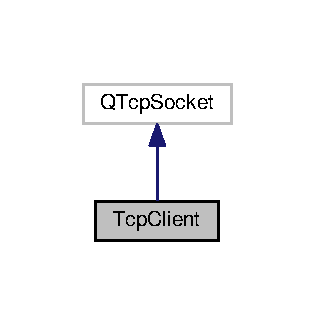
\includegraphics[width=151pt]{class_tcp_client__inherit__graph}
\end{center}
\end{figure}


Collaboration diagram for Tcp\+Client\+:\nopagebreak
\begin{figure}[H]
\begin{center}
\leavevmode
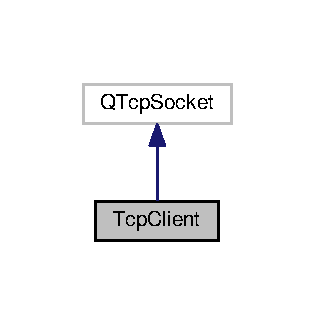
\includegraphics[width=151pt]{class_tcp_client__coll__graph}
\end{center}
\end{figure}
\subsection*{Public Slots}
\begin{DoxyCompactItemize}
\item 
void \mbox{\hyperlink{class_tcp_client_a2c1b8363f05d55bc06335f8da4c7fc8e}{host\+\_\+found\+\_\+handler}} (void)
\begin{DoxyCompactList}\small\item\em Handle host found. \end{DoxyCompactList}\item 
void \mbox{\hyperlink{class_tcp_client_a2467855310250aad604efaabfdccb55c}{connected\+\_\+handler}} (void)
\begin{DoxyCompactList}\small\item\em Handle connection to host. \end{DoxyCompactList}\end{DoxyCompactItemize}
\subsection*{Public Member Functions}
\begin{DoxyCompactItemize}
\item 
\mbox{\hyperlink{class_tcp_client_adde22f7475a79d89eca8107fd9223405}{Tcp\+Client}} (Q\+Tcp\+Socket $\ast$parent=0)
\begin{DoxyCompactList}\small\item\em Builder of the \mbox{\hyperlink{class_tcp_client}{Tcp\+Client}} class. \end{DoxyCompactList}\item 
\mbox{\hyperlink{class_tcp_client_a27a11b182cec604367594ae040e042a8}{Tcp\+Client}} (Q\+Host\+Address host\+\_\+address, quint16 port)
\begin{DoxyCompactList}\small\item\em Builder of the \mbox{\hyperlink{class_tcp_client}{Tcp\+Client}} class. \end{DoxyCompactList}\item 
\mbox{\hyperlink{class_tcp_client_a125d2277f401cbdebadb9689a5933e18}{$\sim$\+Tcp\+Client}} ()
\begin{DoxyCompactList}\small\item\em Destroyer of the \mbox{\hyperlink{class_tcp_client}{Tcp\+Client}} class. \end{DoxyCompactList}\end{DoxyCompactItemize}
\subsection*{Private Attributes}
\begin{DoxyCompactItemize}
\item 
quint16 \mbox{\hyperlink{class_tcp_client_a9c8dbdd8d4571d37bc774d17b627c2d5}{m\+\_\+port}}
\item 
Q\+Host\+Address \mbox{\hyperlink{class_tcp_client_acf0e0d339a1160852fd2ed2eaf4dce7f}{m\+\_\+host\+\_\+address}}
\end{DoxyCompactItemize}


\subsection{Detailed Description}
The \mbox{\hyperlink{class_tcp_client}{Tcp\+Client}} class allow to make usage of Q\+Tcp\+Socket more suitable for development. 

\subsection{Constructor \& Destructor Documentation}
\mbox{\Hypertarget{class_tcp_client_adde22f7475a79d89eca8107fd9223405}\label{class_tcp_client_adde22f7475a79d89eca8107fd9223405}} 
\index{TcpClient@{TcpClient}!TcpClient@{TcpClient}}
\index{TcpClient@{TcpClient}!TcpClient@{TcpClient}}
\subsubsection{\texorpdfstring{TcpClient()}{TcpClient()}\hspace{0.1cm}{\footnotesize\ttfamily [1/2]}}
{\footnotesize\ttfamily Tcp\+Client\+::\+Tcp\+Client (\begin{DoxyParamCaption}\item[{Q\+Tcp\+Socket $\ast$}]{parent = {\ttfamily 0} }\end{DoxyParamCaption})}



Builder of the \mbox{\hyperlink{class_tcp_client}{Tcp\+Client}} class. 


\begin{DoxyParams}{Parameters}
{\em parent} & The parent of the \mbox{\hyperlink{class_tcp_client}{Tcp\+Client}} \\
\hline
\end{DoxyParams}
\mbox{\Hypertarget{class_tcp_client_a27a11b182cec604367594ae040e042a8}\label{class_tcp_client_a27a11b182cec604367594ae040e042a8}} 
\index{TcpClient@{TcpClient}!TcpClient@{TcpClient}}
\index{TcpClient@{TcpClient}!TcpClient@{TcpClient}}
\subsubsection{\texorpdfstring{TcpClient()}{TcpClient()}\hspace{0.1cm}{\footnotesize\ttfamily [2/2]}}
{\footnotesize\ttfamily Tcp\+Client\+::\+Tcp\+Client (\begin{DoxyParamCaption}\item[{Q\+Host\+Address}]{host\+\_\+address,  }\item[{quint16}]{port }\end{DoxyParamCaption})}



Builder of the \mbox{\hyperlink{class_tcp_client}{Tcp\+Client}} class. 


\begin{DoxyParams}{Parameters}
{\em host\+\_\+address} & The address of the server \\
\hline
{\em port} & The port of the server \\
\hline
\end{DoxyParams}
\mbox{\Hypertarget{class_tcp_client_a125d2277f401cbdebadb9689a5933e18}\label{class_tcp_client_a125d2277f401cbdebadb9689a5933e18}} 
\index{TcpClient@{TcpClient}!````~TcpClient@{$\sim$TcpClient}}
\index{````~TcpClient@{$\sim$TcpClient}!TcpClient@{TcpClient}}
\subsubsection{\texorpdfstring{$\sim$TcpClient()}{~TcpClient()}}
{\footnotesize\ttfamily Tcp\+Client\+::$\sim$\+Tcp\+Client (\begin{DoxyParamCaption}{ }\end{DoxyParamCaption})}



Destroyer of the \mbox{\hyperlink{class_tcp_client}{Tcp\+Client}} class. 



\subsection{Member Function Documentation}
\mbox{\Hypertarget{class_tcp_client_a2467855310250aad604efaabfdccb55c}\label{class_tcp_client_a2467855310250aad604efaabfdccb55c}} 
\index{TcpClient@{TcpClient}!connected\_handler@{connected\_handler}}
\index{connected\_handler@{connected\_handler}!TcpClient@{TcpClient}}
\subsubsection{\texorpdfstring{connected\_handler}{connected\_handler}}
{\footnotesize\ttfamily void Tcp\+Client\+::connected\+\_\+handler (\begin{DoxyParamCaption}\item[{void}]{ }\end{DoxyParamCaption})\hspace{0.3cm}{\ttfamily [slot]}}



Handle connection to host. 

\mbox{\Hypertarget{class_tcp_client_a2c1b8363f05d55bc06335f8da4c7fc8e}\label{class_tcp_client_a2c1b8363f05d55bc06335f8da4c7fc8e}} 
\index{TcpClient@{TcpClient}!host\_found\_handler@{host\_found\_handler}}
\index{host\_found\_handler@{host\_found\_handler}!TcpClient@{TcpClient}}
\subsubsection{\texorpdfstring{host\_found\_handler}{host\_found\_handler}}
{\footnotesize\ttfamily void Tcp\+Client\+::host\+\_\+found\+\_\+handler (\begin{DoxyParamCaption}\item[{void}]{ }\end{DoxyParamCaption})\hspace{0.3cm}{\ttfamily [slot]}}



Handle host found. 



\subsection{Member Data Documentation}
\mbox{\Hypertarget{class_tcp_client_acf0e0d339a1160852fd2ed2eaf4dce7f}\label{class_tcp_client_acf0e0d339a1160852fd2ed2eaf4dce7f}} 
\index{TcpClient@{TcpClient}!m\_host\_address@{m\_host\_address}}
\index{m\_host\_address@{m\_host\_address}!TcpClient@{TcpClient}}
\subsubsection{\texorpdfstring{m\_host\_address}{m\_host\_address}}
{\footnotesize\ttfamily Q\+Host\+Address Tcp\+Client\+::m\+\_\+host\+\_\+address\hspace{0.3cm}{\ttfamily [private]}}

server host address \mbox{\Hypertarget{class_tcp_client_a9c8dbdd8d4571d37bc774d17b627c2d5}\label{class_tcp_client_a9c8dbdd8d4571d37bc774d17b627c2d5}} 
\index{TcpClient@{TcpClient}!m\_port@{m\_port}}
\index{m\_port@{m\_port}!TcpClient@{TcpClient}}
\subsubsection{\texorpdfstring{m\_port}{m\_port}}
{\footnotesize\ttfamily quint16 Tcp\+Client\+::m\+\_\+port\hspace{0.3cm}{\ttfamily [private]}}

server port 

The documentation for this class was generated from the following files\+:\begin{DoxyCompactItemize}
\item 
src/network/\mbox{\hyperlink{tcp__client_8hpp}{tcp\+\_\+client.\+hpp}}\item 
src/network/\mbox{\hyperlink{tcp__client_8cpp}{tcp\+\_\+client.\+cpp}}\end{DoxyCompactItemize}

\hypertarget{class_tcp_server}{}\section{Tcp\+Server Class Reference}
\label{class_tcp_server}\index{TcpServer@{TcpServer}}


The \mbox{\hyperlink{class_tcp_server}{Tcp\+Server}} class allow to make usage of Q\+Tcp\+Server more suitable for development.  




{\ttfamily \#include $<$tcp\+\_\+server.\+hpp$>$}



Inheritance diagram for Tcp\+Server\+:\nopagebreak
\begin{figure}[H]
\begin{center}
\leavevmode
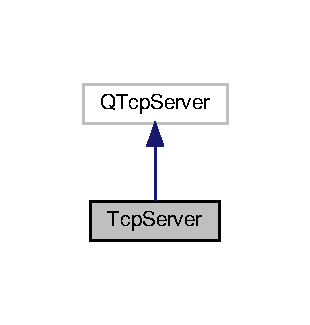
\includegraphics[width=149pt]{d8/dc4/class_tcp_server__inherit__graph}
\end{center}
\end{figure}


Collaboration diagram for Tcp\+Server\+:\nopagebreak
\begin{figure}[H]
\begin{center}
\leavevmode
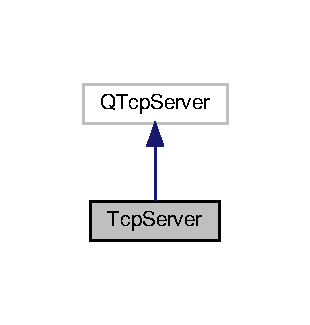
\includegraphics[width=149pt]{dc/d71/class_tcp_server__coll__graph}
\end{center}
\end{figure}
\subsection*{Public Slots}
\begin{DoxyCompactItemize}
\item 
void \mbox{\hyperlink{class_tcp_server_a90ee8945eb2ceec552f5f7a850fd9dce}{create\+\_\+socket}} (void)
\begin{DoxyCompactList}\small\item\em create\+\_\+socket \end{DoxyCompactList}\end{DoxyCompactItemize}
\subsection*{Public Member Functions}
\begin{DoxyCompactItemize}
\item 
\mbox{\hyperlink{class_tcp_server_abc977059ef61f1c42f5fda1bc5945ab0}{Tcp\+Server}} ()
\item 
\mbox{\hyperlink{class_tcp_server_af43d51237b45ebb729911d829dfa7856}{Tcp\+Server}} (bool autostart=0)
\item 
\mbox{\hyperlink{class_tcp_server_a5242d1465353dd6e57bf556416021598}{Tcp\+Server}} (Q\+String \&host\+\_\+address, quint16 port=4444, bool autostart=0)
\item 
\mbox{\hyperlink{class_tcp_server_a728a9e31c53cf86887f1f6149b1c46dd}{$\sim$\+Tcp\+Server}} ()
\item 
void \mbox{\hyperlink{class_tcp_server_ab9a387d38fd311ae853b4b4006504096}{start}} (void)
\begin{DoxyCompactList}\small\item\em start \end{DoxyCompactList}\item 
void \mbox{\hyperlink{class_tcp_server_aaf6005b12641ab81bcf91099d9255437}{set\+\_\+port}} (quint16 port)
\begin{DoxyCompactList}\small\item\em set\+\_\+port \end{DoxyCompactList}\item 
void \mbox{\hyperlink{class_tcp_server_a3496c0dfa5e3c1cb5bf794739508eda4}{set\+\_\+address}} (const char $\ast$address)
\begin{DoxyCompactList}\small\item\em set\+\_\+address \end{DoxyCompactList}\item 
Q\+Tcp\+Socket $\ast$ \mbox{\hyperlink{class_tcp_server_a321f1064fd590efdeb1f9458b89afdca}{get\+\_\+client}} (void)
\begin{DoxyCompactList}\small\item\em get\+\_\+client \end{DoxyCompactList}\end{DoxyCompactItemize}


\subsection{Detailed Description}
The \mbox{\hyperlink{class_tcp_server}{Tcp\+Server}} class allow to make usage of Q\+Tcp\+Server more suitable for development. 

Definition at line 20 of file tcp\+\_\+server.\+hpp.



\subsection{Constructor \& Destructor Documentation}
\mbox{\Hypertarget{class_tcp_server_abc977059ef61f1c42f5fda1bc5945ab0}\label{class_tcp_server_abc977059ef61f1c42f5fda1bc5945ab0}} 
\index{TcpServer@{TcpServer}!TcpServer@{TcpServer}}
\index{TcpServer@{TcpServer}!TcpServer@{TcpServer}}
\subsubsection{\texorpdfstring{TcpServer()}{TcpServer()}\hspace{0.1cm}{\footnotesize\ttfamily [1/3]}}
{\footnotesize\ttfamily Tcp\+Server\+::\+Tcp\+Server (\begin{DoxyParamCaption}{ }\end{DoxyParamCaption})\hspace{0.3cm}{\ttfamily [explicit]}}



Definition at line 3 of file tcp\+\_\+server.\+cpp.


\begin{DoxyCode}{0}
\DoxyCodeLine{3                     \{}
\DoxyCodeLine{4 }
\DoxyCodeLine{5 \}}

\end{DoxyCode}
\mbox{\Hypertarget{class_tcp_server_af43d51237b45ebb729911d829dfa7856}\label{class_tcp_server_af43d51237b45ebb729911d829dfa7856}} 
\index{TcpServer@{TcpServer}!TcpServer@{TcpServer}}
\index{TcpServer@{TcpServer}!TcpServer@{TcpServer}}
\subsubsection{\texorpdfstring{TcpServer()}{TcpServer()}\hspace{0.1cm}{\footnotesize\ttfamily [2/3]}}
{\footnotesize\ttfamily Tcp\+Server\+::\+Tcp\+Server (\begin{DoxyParamCaption}\item[{bool}]{autostart = {\ttfamily 0} }\end{DoxyParamCaption})}



Definition at line 7 of file tcp\+\_\+server.\+cpp.


\begin{DoxyCode}{0}
\DoxyCodeLine{7                                   \{}
\DoxyCodeLine{8     m\_host\_address = \textcolor{stringliteral}{"127.0.0.1"};}
\DoxyCodeLine{9     m\_port = 4444;}
\DoxyCodeLine{10 }
\DoxyCodeLine{11     \textcolor{keywordflow}{if} (autostart)\{}
\DoxyCodeLine{12         \mbox{\hyperlink{class_tcp_server_ab9a387d38fd311ae853b4b4006504096}{start}}();}
\DoxyCodeLine{13     \}}
\DoxyCodeLine{14 \}}

\end{DoxyCode}
\mbox{\Hypertarget{class_tcp_server_a5242d1465353dd6e57bf556416021598}\label{class_tcp_server_a5242d1465353dd6e57bf556416021598}} 
\index{TcpServer@{TcpServer}!TcpServer@{TcpServer}}
\index{TcpServer@{TcpServer}!TcpServer@{TcpServer}}
\subsubsection{\texorpdfstring{TcpServer()}{TcpServer()}\hspace{0.1cm}{\footnotesize\ttfamily [3/3]}}
{\footnotesize\ttfamily Tcp\+Server\+::\+Tcp\+Server (\begin{DoxyParamCaption}\item[{Q\+String \&}]{host\+\_\+address,  }\item[{quint16}]{port = {\ttfamily 4444},  }\item[{bool}]{autostart = {\ttfamily 0} }\end{DoxyParamCaption})}



Definition at line 16 of file tcp\+\_\+server.\+cpp.


\begin{DoxyCode}{0}
\DoxyCodeLine{16                                                                        \{}
\DoxyCodeLine{17     m\_host\_address = host\_address;}
\DoxyCodeLine{18     m\_port = port;}
\DoxyCodeLine{19 }
\DoxyCodeLine{20     \textcolor{keywordflow}{if} (autostart)\{}
\DoxyCodeLine{21         \mbox{\hyperlink{class_tcp_server_ab9a387d38fd311ae853b4b4006504096}{start}}();}
\DoxyCodeLine{22     \}}
\DoxyCodeLine{23 \}}

\end{DoxyCode}
\mbox{\Hypertarget{class_tcp_server_a728a9e31c53cf86887f1f6149b1c46dd}\label{class_tcp_server_a728a9e31c53cf86887f1f6149b1c46dd}} 
\index{TcpServer@{TcpServer}!````~TcpServer@{$\sim$TcpServer}}
\index{````~TcpServer@{$\sim$TcpServer}!TcpServer@{TcpServer}}
\subsubsection{\texorpdfstring{$\sim$TcpServer()}{~TcpServer()}}
{\footnotesize\ttfamily Tcp\+Server\+::$\sim$\+Tcp\+Server (\begin{DoxyParamCaption}{ }\end{DoxyParamCaption})}



Definition at line 25 of file tcp\+\_\+server.\+cpp.


\begin{DoxyCode}{0}
\DoxyCodeLine{25                      \{}
\DoxyCodeLine{26 }
\DoxyCodeLine{27 \}}

\end{DoxyCode}


\subsection{Member Function Documentation}
\mbox{\Hypertarget{class_tcp_server_a90ee8945eb2ceec552f5f7a850fd9dce}\label{class_tcp_server_a90ee8945eb2ceec552f5f7a850fd9dce}} 
\index{TcpServer@{TcpServer}!create\_socket@{create\_socket}}
\index{create\_socket@{create\_socket}!TcpServer@{TcpServer}}
\subsubsection{\texorpdfstring{create\_socket}{create\_socket}}
{\footnotesize\ttfamily void Tcp\+Server\+::create\+\_\+socket (\begin{DoxyParamCaption}\item[{void}]{ }\end{DoxyParamCaption})\hspace{0.3cm}{\ttfamily [slot]}}



create\+\_\+socket 



Definition at line 29 of file tcp\+\_\+server.\+cpp.


\begin{DoxyCode}{0}
\DoxyCodeLine{29                              \{}
\DoxyCodeLine{30     m\_tcp\_client = nextPendingConnection();}
\DoxyCodeLine{31 }
\DoxyCodeLine{32     \textcolor{keywordflow}{if} (!m\_tcp\_client->isValid())\{}
\DoxyCodeLine{33         qDebug() << \textcolor{stringliteral}{"TCP socket error: socket state: "} << m\_tcp\_client->state();}
\DoxyCodeLine{34     \}}
\DoxyCodeLine{35 }
\DoxyCodeLine{36     \textcolor{comment}{//connect(m\_tcp\_client, SIGNAL(readyRead()), this, SLOT());}}
\DoxyCodeLine{37 }
\DoxyCodeLine{38     qDebug() << \textcolor{stringliteral}{"Connection opened"};}
\DoxyCodeLine{39 \}}

\end{DoxyCode}
\mbox{\Hypertarget{class_tcp_server_a321f1064fd590efdeb1f9458b89afdca}\label{class_tcp_server_a321f1064fd590efdeb1f9458b89afdca}} 
\index{TcpServer@{TcpServer}!get\_client@{get\_client}}
\index{get\_client@{get\_client}!TcpServer@{TcpServer}}
\subsubsection{\texorpdfstring{get\_client()}{get\_client()}}
{\footnotesize\ttfamily Q\+Tcp\+Socket $\ast$ Tcp\+Server\+::get\+\_\+client (\begin{DoxyParamCaption}\item[{void}]{ }\end{DoxyParamCaption})}



get\+\_\+client 

\begin{DoxyReturn}{Returns}
client address for interacting with the client connected to the server 
\end{DoxyReturn}


Definition at line 68 of file tcp\+\_\+server.\+cpp.


\begin{DoxyCode}{0}
\DoxyCodeLine{68                                      \{}
\DoxyCodeLine{69     \textcolor{keywordflow}{return} m\_tcp\_client;}
\DoxyCodeLine{70 \}}

\end{DoxyCode}
\mbox{\Hypertarget{class_tcp_server_a3496c0dfa5e3c1cb5bf794739508eda4}\label{class_tcp_server_a3496c0dfa5e3c1cb5bf794739508eda4}} 
\index{TcpServer@{TcpServer}!set\_address@{set\_address}}
\index{set\_address@{set\_address}!TcpServer@{TcpServer}}
\subsubsection{\texorpdfstring{set\_address()}{set\_address()}}
{\footnotesize\ttfamily void Tcp\+Server\+::set\+\_\+address (\begin{DoxyParamCaption}\item[{const char $\ast$}]{address }\end{DoxyParamCaption})}



set\+\_\+address 


\begin{DoxyParams}{Parameters}
{\em address} & \\
\hline
\end{DoxyParams}


Definition at line 64 of file tcp\+\_\+server.\+cpp.


\begin{DoxyCode}{0}
\DoxyCodeLine{64                                               \{}
\DoxyCodeLine{65     m\_host\_address = QString(address);}
\DoxyCodeLine{66 \}}

\end{DoxyCode}
\mbox{\Hypertarget{class_tcp_server_aaf6005b12641ab81bcf91099d9255437}\label{class_tcp_server_aaf6005b12641ab81bcf91099d9255437}} 
\index{TcpServer@{TcpServer}!set\_port@{set\_port}}
\index{set\_port@{set\_port}!TcpServer@{TcpServer}}
\subsubsection{\texorpdfstring{set\_port()}{set\_port()}}
{\footnotesize\ttfamily void Tcp\+Server\+::set\+\_\+port (\begin{DoxyParamCaption}\item[{quint16}]{port }\end{DoxyParamCaption})}



set\+\_\+port 


\begin{DoxyParams}{Parameters}
{\em port} & \\
\hline
\end{DoxyParams}


Definition at line 60 of file tcp\+\_\+server.\+cpp.


\begin{DoxyCode}{0}
\DoxyCodeLine{60                                     \{}
\DoxyCodeLine{61     m\_port = port;}
\DoxyCodeLine{62 \}}

\end{DoxyCode}
\mbox{\Hypertarget{class_tcp_server_ab9a387d38fd311ae853b4b4006504096}\label{class_tcp_server_ab9a387d38fd311ae853b4b4006504096}} 
\index{TcpServer@{TcpServer}!start@{start}}
\index{start@{start}!TcpServer@{TcpServer}}
\subsubsection{\texorpdfstring{start()}{start()}}
{\footnotesize\ttfamily void Tcp\+Server\+::start (\begin{DoxyParamCaption}\item[{void}]{ }\end{DoxyParamCaption})}



start 



Definition at line 41 of file tcp\+\_\+server.\+cpp.


\begin{DoxyCode}{0}
\DoxyCodeLine{41                      \{}
\DoxyCodeLine{42     \textcolor{keywordtype}{bool} ret = \textcolor{keyword}{false};}
\DoxyCodeLine{43 }
\DoxyCodeLine{44     qDebug() << \textcolor{stringliteral}{"Starting TCP server..."};}
\DoxyCodeLine{45 }
\DoxyCodeLine{46     connect(\textcolor{keyword}{this}, SIGNAL(newConnection()), \textcolor{keyword}{this}, SLOT(\mbox{\hyperlink{class_tcp_server_a90ee8945eb2ceec552f5f7a850fd9dce}{create\_socket}}()));}
\DoxyCodeLine{47 }
\DoxyCodeLine{48     \textcolor{comment}{// Get host address automatically whether possible}}
\DoxyCodeLine{49     ret = listen(QHostAddress(QString(m\_host\_address)), m\_port);}
\DoxyCodeLine{50 }
\DoxyCodeLine{51     \textcolor{keywordflow}{if} (ret == \textcolor{keyword}{false})\{}
\DoxyCodeLine{52         qDebug() << \textcolor{stringliteral}{"Starting TCP server... failed"};}
\DoxyCodeLine{53     \}}
\DoxyCodeLine{54 }
\DoxyCodeLine{55     \textcolor{comment}{// Wait until isListening() with timeout}}
\DoxyCodeLine{56 }
\DoxyCodeLine{57     qDebug() << \textcolor{stringliteral}{"Starting TCP server... done"};}
\DoxyCodeLine{58 \}}

\end{DoxyCode}


The documentation for this class was generated from the following files\+:\begin{DoxyCompactItemize}
\item 
network/\mbox{\hyperlink{tcp__server_8hpp}{tcp\+\_\+server.\+hpp}}\item 
network/\mbox{\hyperlink{tcp__server_8cpp}{tcp\+\_\+server.\+cpp}}\end{DoxyCompactItemize}

\chapter{File Documentation}
\hypertarget{_autoscope_8cpp}{}\section{Autoscope.\+cpp File Reference}
\label{_autoscope_8cpp}\index{Autoscope.cpp@{Autoscope.cpp}}
{\ttfamily \#include \char`\"{}Stel\+Projector.\+hpp\char`\"{}}\newline
{\ttfamily \#include \char`\"{}Stel\+Painter.\+hpp\char`\"{}}\newline
{\ttfamily \#include \char`\"{}Stel\+App.\+hpp\char`\"{}}\newline
{\ttfamily \#include \char`\"{}Stel\+Core.\+hpp\char`\"{}}\newline
{\ttfamily \#include \char`\"{}Stel\+Locale\+Mgr.\+hpp\char`\"{}}\newline
{\ttfamily \#include \char`\"{}Stel\+Module\+Mgr.\+hpp\char`\"{}}\newline
{\ttfamily \#include \char`\"{}Autoscope.\+hpp\char`\"{}}\newline
{\ttfamily \#include \char`\"{}Stel\+Utils.\+hpp\char`\"{}}\newline
{\ttfamily \#include \char`\"{}Stel\+Object\+Type.\+hpp\char`\"{}}\newline
{\ttfamily \#include \char`\"{}Stel\+Movement\+Mgr.\+hpp\char`\"{}}\newline
{\ttfamily \#include \char`\"{}Stel\+Object\+Mgr.\+hpp\char`\"{}}\newline
{\ttfamily \#include \char`\"{}Stel\+Gui.\+hpp\char`\"{}}\newline
{\ttfamily \#include \char`\"{}Stel\+Gui\+Items.\+hpp\char`\"{}}\newline
{\ttfamily \#include \char`\"{}Stel\+File\+Mgr.\+hpp\char`\"{}}\newline
{\ttfamily \#include $<$Q\+Pixmap$>$}\newline
{\ttfamily \#include $<$Q\+Settings$>$}\newline
{\ttfamily \#include \char`\"{}Stel\+Dialog.\+hpp\char`\"{}}\newline
{\ttfamily \#include \char`\"{}Autoscope\+Window\+Form.\+hpp\char`\"{}}\newline
{\ttfamily \#include \char`\"{}Autoscope\+Picture\+Window\+Form.\+hpp\char`\"{}}\newline
{\ttfamily \#include \char`\"{}network/tcp\+\_\+client.\+hpp\char`\"{}}\newline
{\ttfamily \#include $<$Q\+Desktop\+Widget$>$}\newline
{\ttfamily \#include $<$Q\+Debug$>$}\newline
Include dependency graph for Autoscope.\+cpp\+:\nopagebreak
\begin{figure}[H]
\begin{center}
\leavevmode
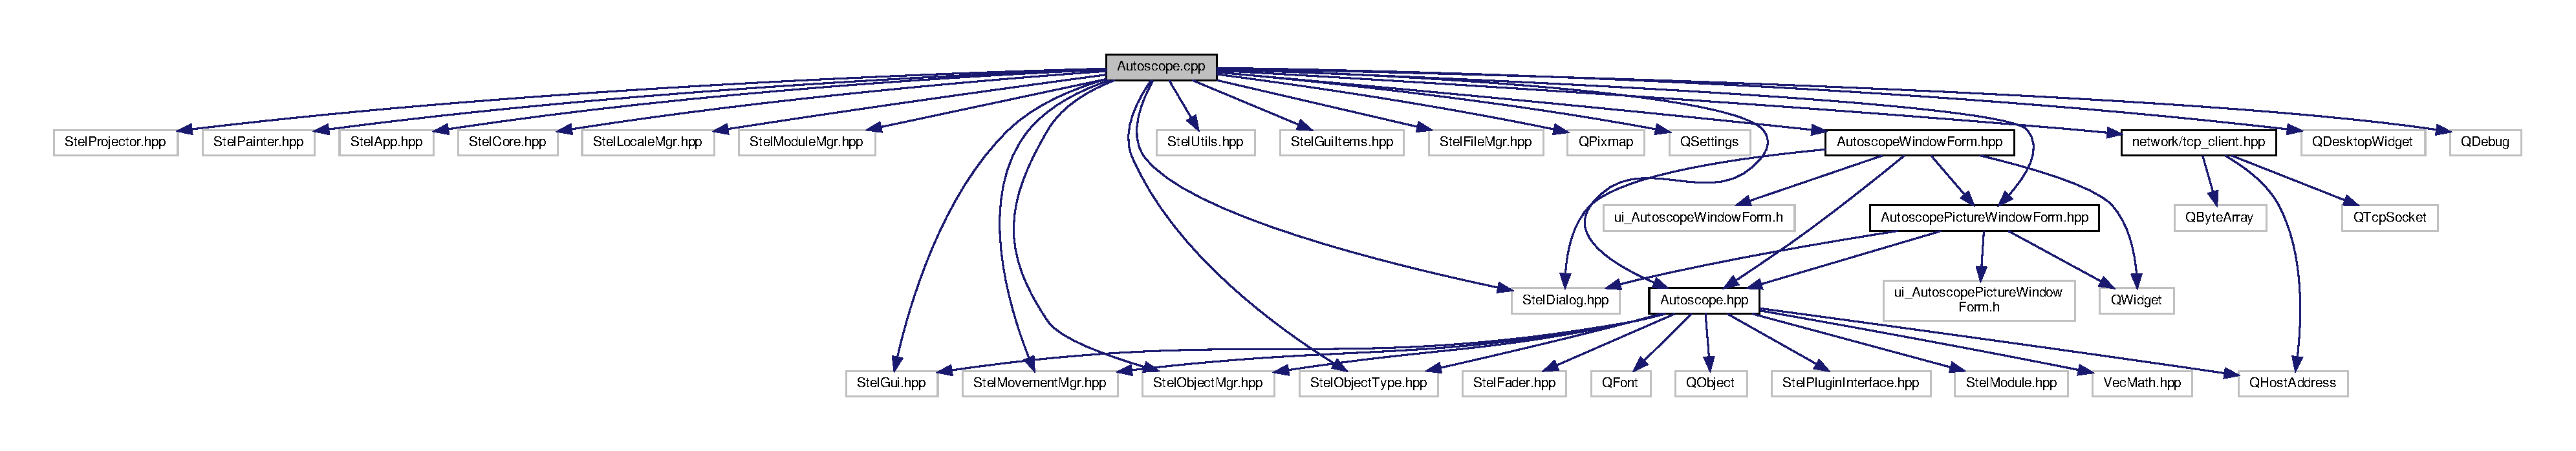
\includegraphics[width=350pt]{d6/d4b/_autoscope_8cpp__incl}
\end{center}
\end{figure}

\hypertarget{_autoscope_8hpp}{}\section{src/\+Autoscope.hpp File Reference}
\label{_autoscope_8hpp}\index{src/Autoscope.hpp@{src/Autoscope.hpp}}


Main plugin class.  


{\ttfamily \#include \char`\"{}Stel\+Module.\+hpp\char`\"{}}\newline
{\ttfamily \#include \char`\"{}Stel\+Gui.\+hpp\char`\"{}}\newline
{\ttfamily \#include \char`\"{}Vec\+Math.\+hpp\char`\"{}}\newline
{\ttfamily \#include \char`\"{}Stel\+Fader.\+hpp\char`\"{}}\newline
{\ttfamily \#include $<$Q\+Font$>$}\newline
{\ttfamily \#include \char`\"{}Stel\+Movement\+Mgr.\+hpp\char`\"{}}\newline
{\ttfamily \#include \char`\"{}Stel\+Object\+Mgr.\+hpp\char`\"{}}\newline
{\ttfamily \#include \char`\"{}Stel\+Object\+Type.\+hpp\char`\"{}}\newline
{\ttfamily \#include $<$Q\+Host\+Address$>$}\newline
{\ttfamily \#include $<$Q\+Object$>$}\newline
{\ttfamily \#include \char`\"{}Stel\+Plugin\+Interface.\+hpp\char`\"{}}\newline
Include dependency graph for Autoscope.\+hpp\+:
\nopagebreak
\begin{figure}[H]
\begin{center}
\leavevmode
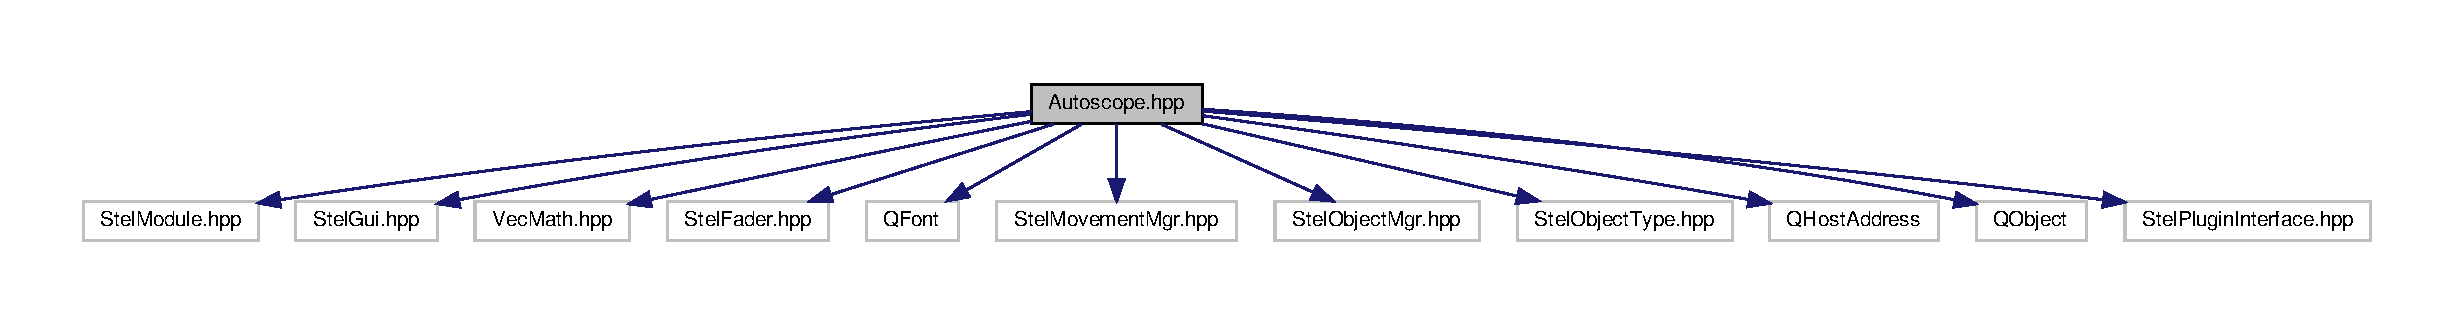
\includegraphics[width=350pt]{_autoscope_8hpp__incl}
\end{center}
\end{figure}
This graph shows which files directly or indirectly include this file\+:
\nopagebreak
\begin{figure}[H]
\begin{center}
\leavevmode
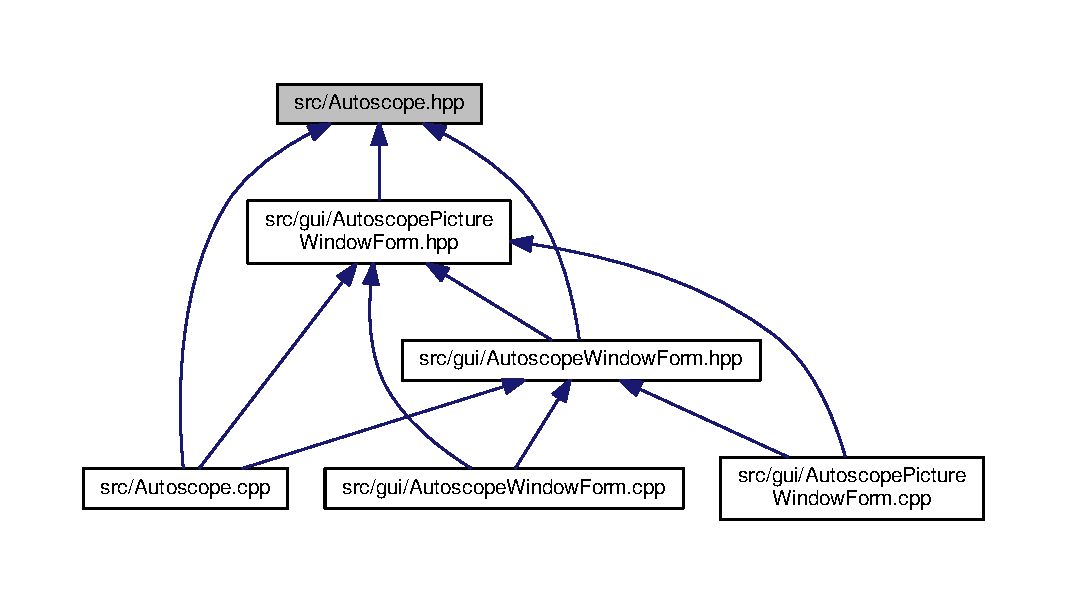
\includegraphics[width=350pt]{_autoscope_8hpp__dep__incl}
\end{center}
\end{figure}
\subsection*{Classes}
\begin{DoxyCompactItemize}
\item 
class \mbox{\hyperlink{class_autoscope}{Autoscope}}
\begin{DoxyCompactList}\small\item\em This class is use to retrieve and compute data for sending to the telescope, and call user interfaces windows. \end{DoxyCompactList}\item 
class \mbox{\hyperlink{class_autoscope_stel_plugin_interface}{Autoscope\+Stel\+Plugin\+Interface}}
\begin{DoxyCompactList}\small\item\em This class is used by Qt to manage a plug-\/in interface. \end{DoxyCompactList}\end{DoxyCompactItemize}


\subsection{Detailed Description}
Main plugin class. 

\begin{DoxyAuthor}{Author}
thibaud-\/ledoledec 
\end{DoxyAuthor}

\hypertarget{_autoscope_picture_window_form_8cpp}{}\section{src/gui/\+Autoscope\+Picture\+Window\+Form.cpp File Reference}
\label{_autoscope_picture_window_form_8cpp}\index{src/gui/AutoscopePictureWindowForm.cpp@{src/gui/AutoscopePictureWindowForm.cpp}}
{\ttfamily \#include \char`\"{}Autoscope\+Picture\+Window\+Form.\+hpp\char`\"{}}\newline
{\ttfamily \#include \char`\"{}ui\+\_\+\+Autoscope\+Picture\+Window\+Form.\+h\char`\"{}}\newline
{\ttfamily \#include \char`\"{}Autoscope\+Window\+Form.\+hpp\char`\"{}}\newline
{\ttfamily \#include \char`\"{}Stel\+Module.\+hpp\char`\"{}}\newline
{\ttfamily \#include \char`\"{}Stel\+Module\+Mgr.\+hpp\char`\"{}}\newline
{\ttfamily \#include $<$Q\+Debug$>$}\newline
Include dependency graph for Autoscope\+Picture\+Window\+Form.\+cpp\+:
\nopagebreak
\begin{figure}[H]
\begin{center}
\leavevmode
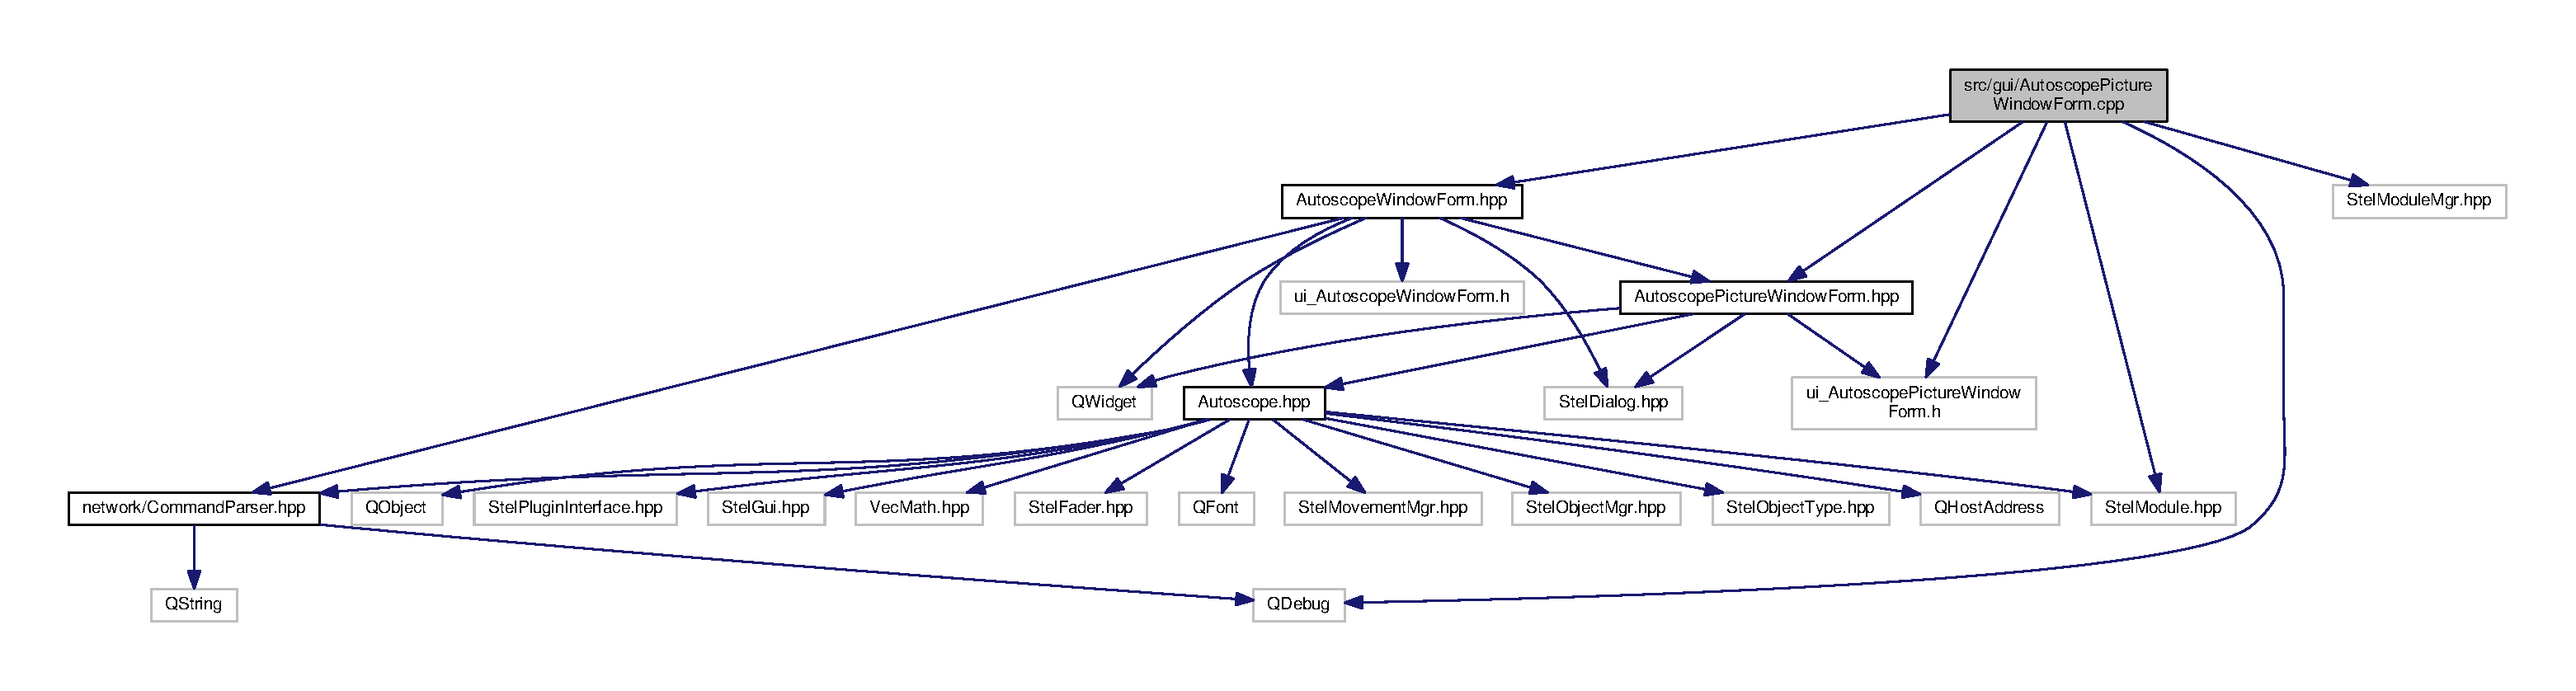
\includegraphics[width=350pt]{_autoscope_picture_window_form_8cpp__incl}
\end{center}
\end{figure}

\hypertarget{_autoscope_picture_window_form_8hpp}{}\section{src/gui/\+Autoscope\+Picture\+Window\+Form.hpp File Reference}
\label{_autoscope_picture_window_form_8hpp}\index{src/gui/AutoscopePictureWindowForm.hpp@{src/gui/AutoscopePictureWindowForm.hpp}}


Header file including the picture display window definition.  


{\ttfamily \#include $<$Q\+Widget$>$}\newline
{\ttfamily \#include \char`\"{}Stel\+Dialog.\+hpp\char`\"{}}\newline
{\ttfamily \#include \char`\"{}Autoscope.\+hpp\char`\"{}}\newline
{\ttfamily \#include \char`\"{}ui\+\_\+\+Autoscope\+Picture\+Window\+Form.\+h\char`\"{}}\newline
Include dependency graph for Autoscope\+Picture\+Window\+Form.\+hpp\+:
\nopagebreak
\begin{figure}[H]
\begin{center}
\leavevmode
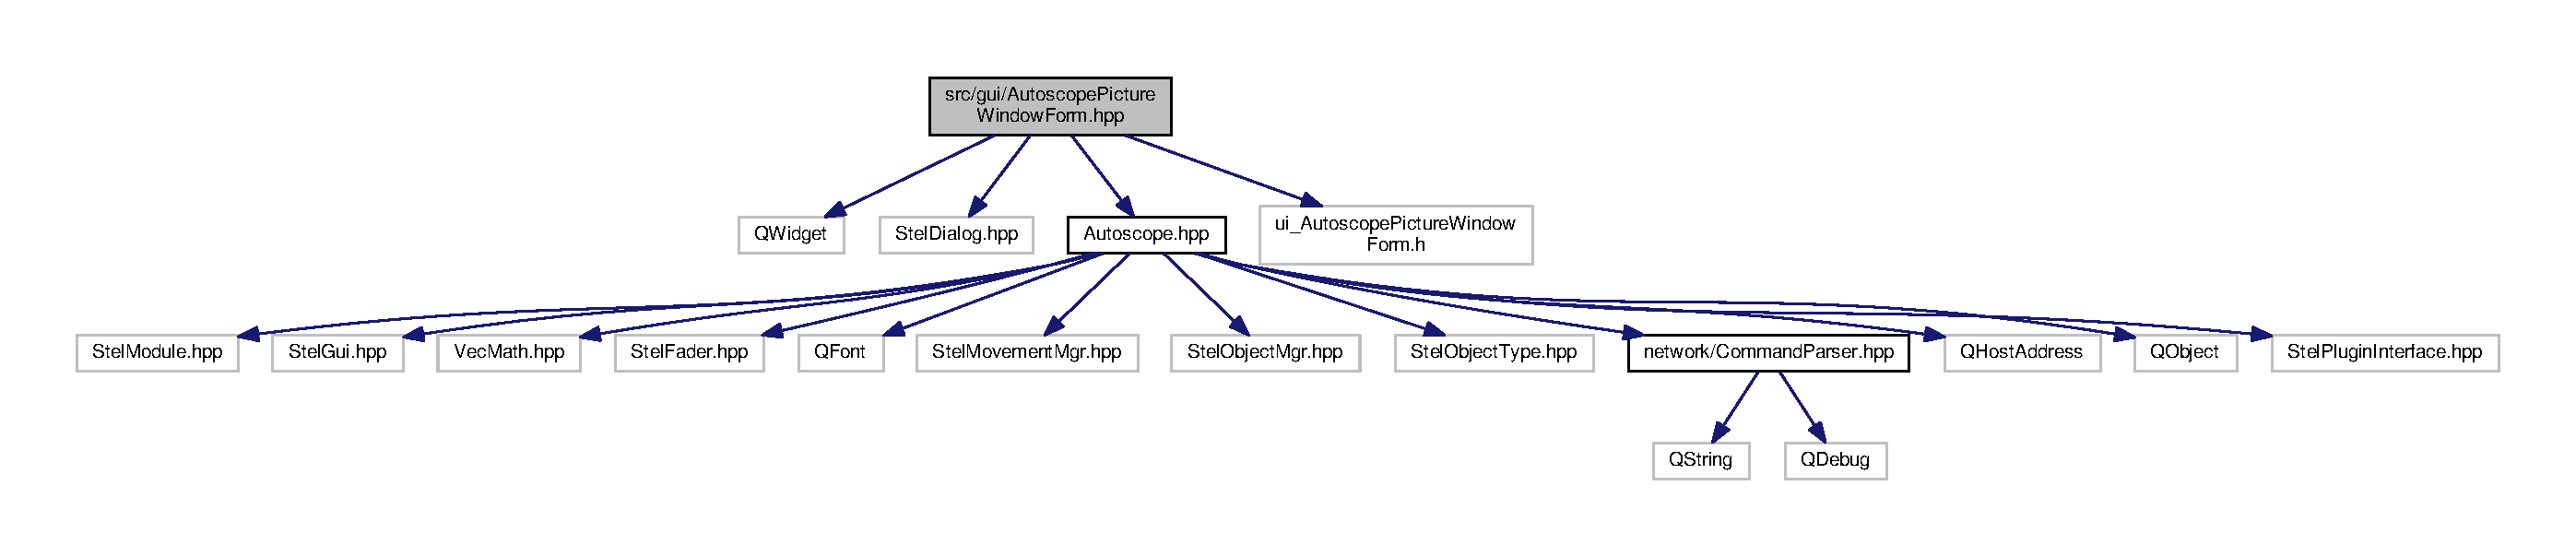
\includegraphics[width=350pt]{_autoscope_picture_window_form_8hpp__incl}
\end{center}
\end{figure}
This graph shows which files directly or indirectly include this file\+:
\nopagebreak
\begin{figure}[H]
\begin{center}
\leavevmode
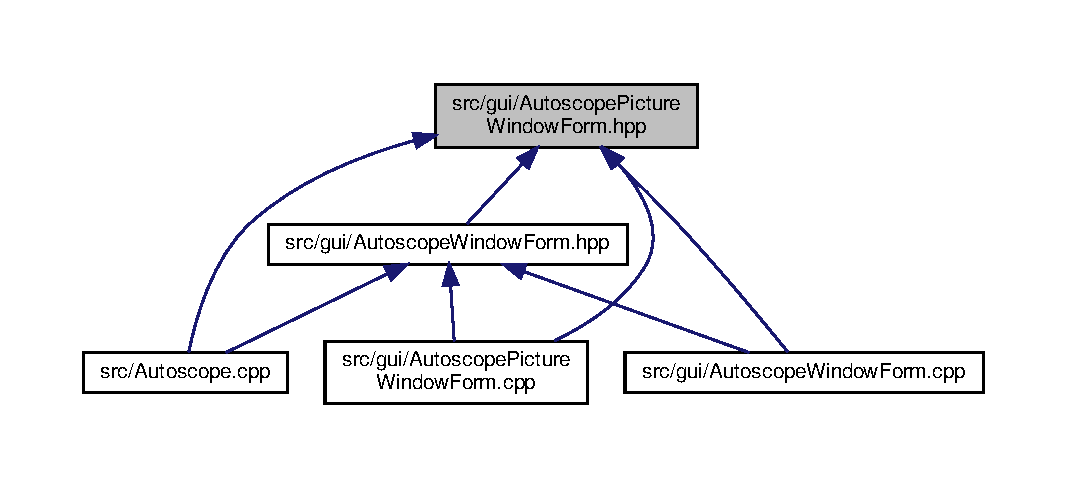
\includegraphics[width=350pt]{_autoscope_picture_window_form_8hpp__dep__incl}
\end{center}
\end{figure}
\subsection*{Classes}
\begin{DoxyCompactItemize}
\item 
class \mbox{\hyperlink{class_autoscope_picture_window_form}{Autoscope\+Picture\+Window\+Form}}
\begin{DoxyCompactList}\small\item\em This class is use to build a picture display interface to show to the user the last taken picture. \end{DoxyCompactList}\end{DoxyCompactItemize}


\subsection{Detailed Description}
Header file including the picture display window definition. 

\begin{DoxyAuthor}{Author}
thibaud-\/ledoledec 
\end{DoxyAuthor}

\hypertarget{_autoscope_window_form_8cpp}{}\section{gui/\+Autoscope\+Window\+Form.cpp File Reference}
\label{_autoscope_window_form_8cpp}\index{gui/AutoscopeWindowForm.cpp@{gui/AutoscopeWindowForm.cpp}}
{\ttfamily \#include \char`\"{}Autoscope\+Window\+Form.\+hpp\char`\"{}}\newline
{\ttfamily \#include \char`\"{}ui\+\_\+\+Autoscope\+Window\+Form.\+h\char`\"{}}\newline
{\ttfamily \#include $<$Q\+Debug$>$}\newline
{\ttfamily \#include $<$Q\+File\+Dialog$>$}\newline
{\ttfamily \#include \char`\"{}Autoscope\+Picture\+Window\+Form.\+hpp\char`\"{}}\newline
{\ttfamily \#include \char`\"{}Stel\+Module.\+hpp\char`\"{}}\newline
{\ttfamily \#include \char`\"{}Stel\+Module\+Mgr.\+hpp\char`\"{}}\newline
Include dependency graph for Autoscope\+Window\+Form.\+cpp\+:\nopagebreak
\begin{figure}[H]
\begin{center}
\leavevmode
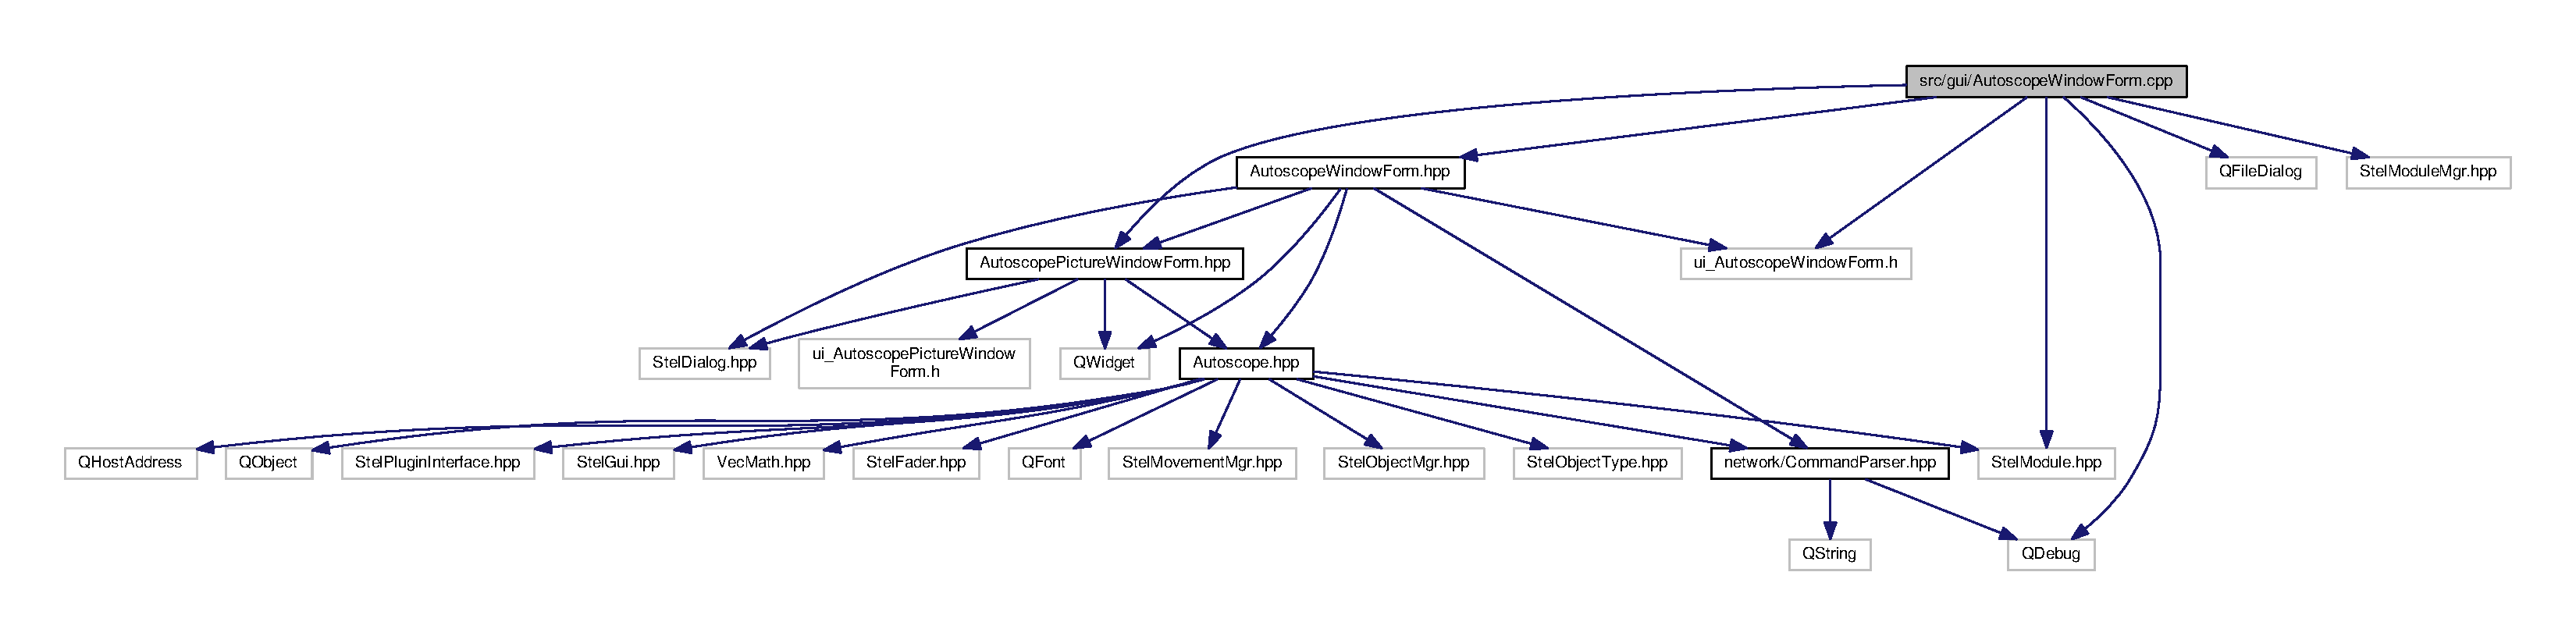
\includegraphics[width=350pt]{_autoscope_window_form_8cpp__incl}
\end{center}
\end{figure}

\hypertarget{_autoscope_window_form_8hpp}{}\section{src/gui/\+Autoscope\+Window\+Form.hpp File Reference}
\label{_autoscope_window_form_8hpp}\index{src/gui/\+Autoscope\+Window\+Form.\+hpp@{src/gui/\+Autoscope\+Window\+Form.\+hpp}}


Header file including configuration window definition.  


{\ttfamily \#include $<$Q\+Widget$>$}\\*
{\ttfamily \#include \char`\"{}Stel\+Dialog.\+hpp\char`\"{}}\\*
{\ttfamily \#include \char`\"{}Autoscope.\+hpp\char`\"{}}\\*
{\ttfamily \#include \char`\"{}ui\+\_\+\+Autoscope\+Window\+Form.\+h\char`\"{}}\\*
{\ttfamily \#include \char`\"{}Autoscope\+Picture\+Window\+Form.\+hpp\char`\"{}}\\*
{\ttfamily \#include \char`\"{}network/\+Command\+Parser.\+hpp\char`\"{}}\\*
Include dependency graph for Autoscope\+Window\+Form.\+hpp\+:
\nopagebreak
\begin{figure}[H]
\begin{center}
\leavevmode
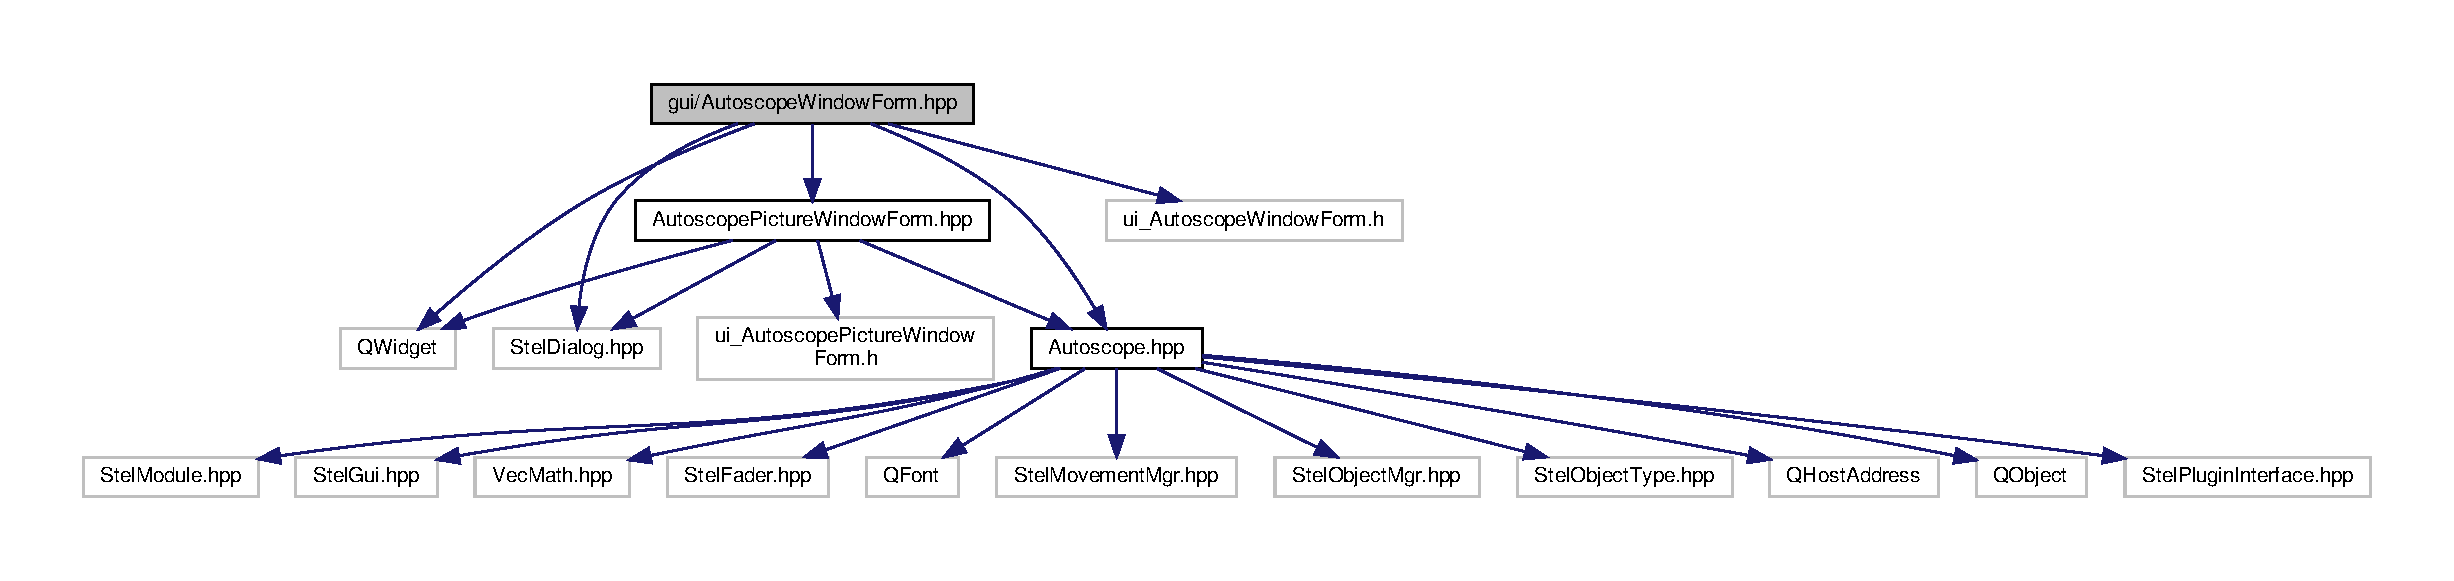
\includegraphics[width=350pt]{_autoscope_window_form_8hpp__incl}
\end{center}
\end{figure}
This graph shows which files directly or indirectly include this file\+:
\nopagebreak
\begin{figure}[H]
\begin{center}
\leavevmode
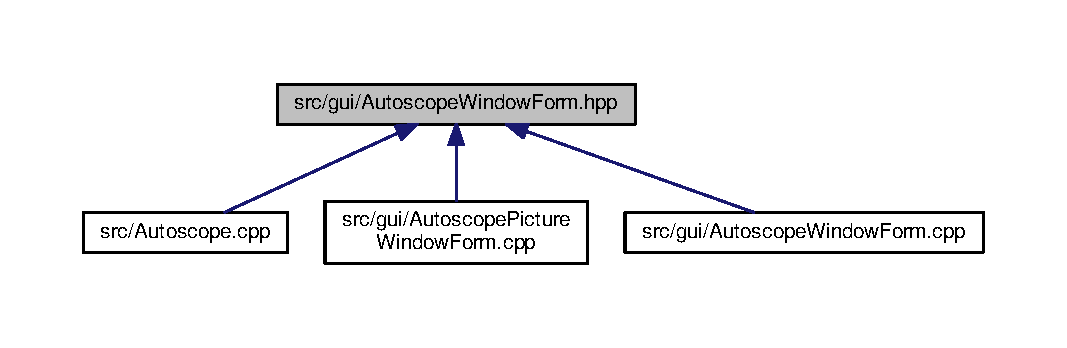
\includegraphics[width=350pt]{_autoscope_window_form_8hpp__dep__incl}
\end{center}
\end{figure}
\subsection*{Classes}
\begin{DoxyCompactItemize}
\item 
class \hyperlink{class_autoscope_window_form}{Autoscope\+Window\+Form}
\begin{DoxyCompactList}\small\item\em This class is use to build a configuration interface between the user and the plugin. \end{DoxyCompactList}\end{DoxyCompactItemize}


\subsection{Detailed Description}
Header file including configuration window definition. 

\begin{DoxyAuthor}{Author}
thibaud-\/ledoledec 
\end{DoxyAuthor}

\hypertarget{_command_parser_8cpp}{}\section{src/network/\+Command\+Parser.cpp File Reference}
\label{_command_parser_8cpp}\index{src/network/\+Command\+Parser.\+cpp@{src/network/\+Command\+Parser.\+cpp}}
{\ttfamily \#include \char`\"{}Command\+Parser.\+hpp\char`\"{}}\\*
Include dependency graph for Command\+Parser.\+cpp\+:
\nopagebreak
\begin{figure}[H]
\begin{center}
\leavevmode
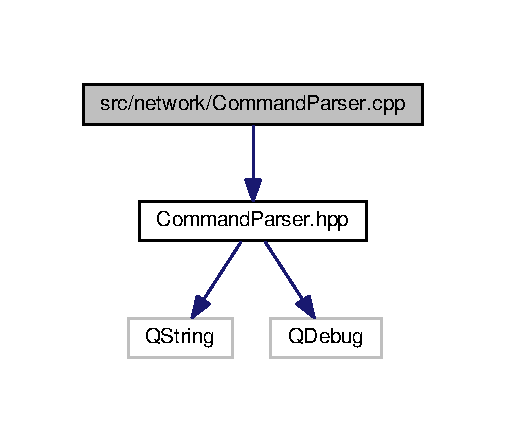
\includegraphics[width=243pt]{_command_parser_8cpp__incl}
\end{center}
\end{figure}

\hypertarget{_command_parser_8hpp}{}\section{src/network/\+Command\+Parser.hpp File Reference}
\label{_command_parser_8hpp}\index{src/network/\+Command\+Parser.\+hpp@{src/network/\+Command\+Parser.\+hpp}}
{\ttfamily \#include $<$Q\+String$>$}\\*
{\ttfamily \#include $<$Q\+Debug$>$}\\*
Include dependency graph for Command\+Parser.\+hpp\+:
\nopagebreak
\begin{figure}[H]
\begin{center}
\leavevmode
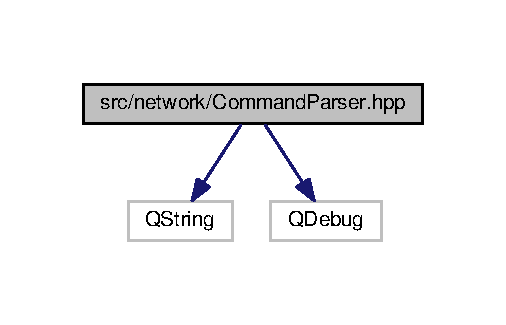
\includegraphics[width=243pt]{_command_parser_8hpp__incl}
\end{center}
\end{figure}
This graph shows which files directly or indirectly include this file\+:
\nopagebreak
\begin{figure}[H]
\begin{center}
\leavevmode
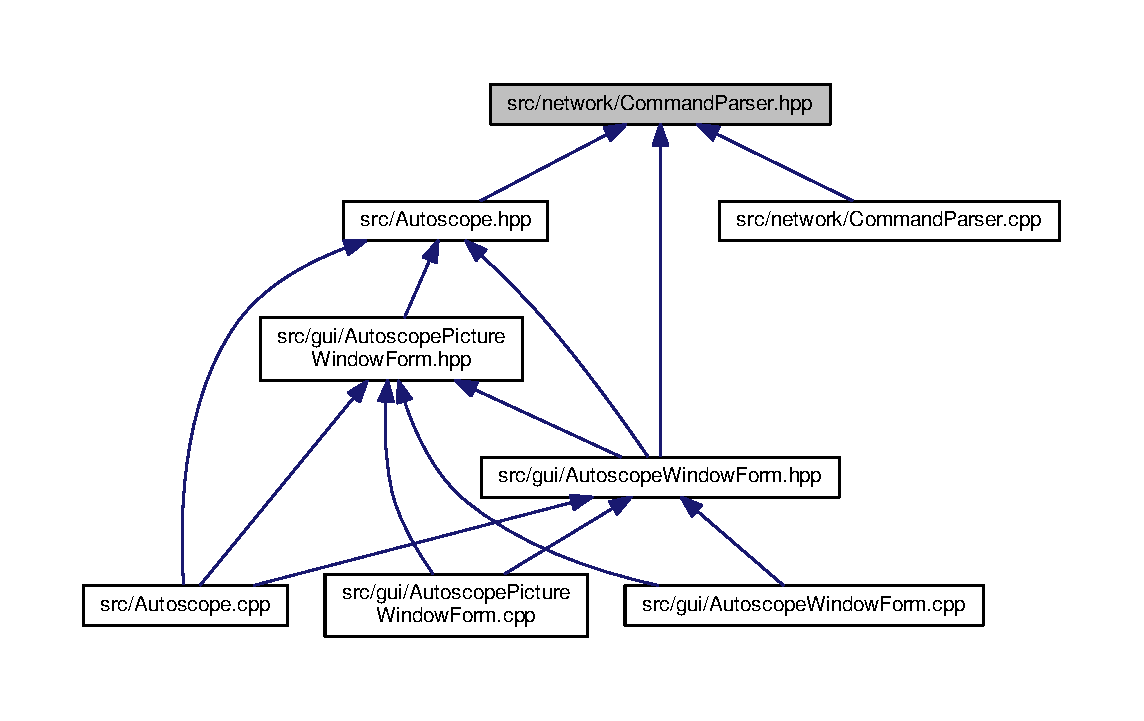
\includegraphics[width=350pt]{_command_parser_8hpp__dep__incl}
\end{center}
\end{figure}
\subsection*{Classes}
\begin{DoxyCompactItemize}
\item 
class \hyperlink{class_command_parser}{Command\+Parser}
\end{DoxyCompactItemize}

\hypertarget{tcp__client_8cpp}{}\section{network/tcp\+\_\+client.cpp File Reference}
\label{tcp__client_8cpp}\index{network/tcp\_client.cpp@{network/tcp\_client.cpp}}
{\ttfamily \#include \char`\"{}tcp\+\_\+client.\+hpp\char`\"{}}\newline
Include dependency graph for tcp\+\_\+client.\+cpp\+:\nopagebreak
\begin{figure}[H]
\begin{center}
\leavevmode
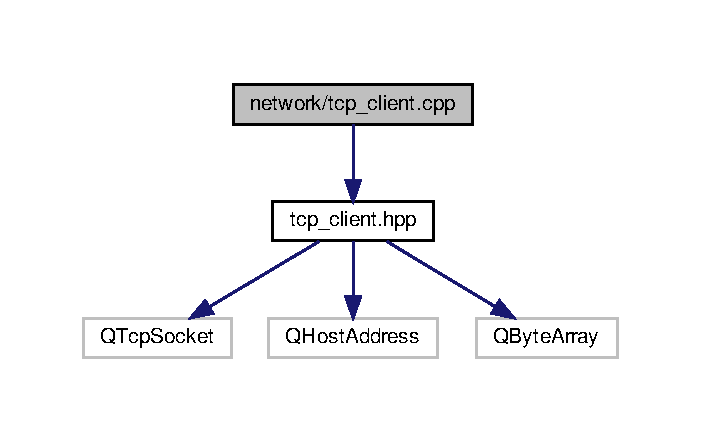
\includegraphics[width=337pt]{d3/d27/tcp__client_8cpp__incl}
\end{center}
\end{figure}

\hypertarget{tcp__client_8hpp}{}\section{src/network/tcp\+\_\+client.hpp File Reference}
\label{tcp__client_8hpp}\index{src/network/tcp\+\_\+client.\+hpp@{src/network/tcp\+\_\+client.\+hpp}}


Header file including T\+CP client definition.  


{\ttfamily \#include $<$Q\+Tcp\+Socket$>$}\\*
{\ttfamily \#include $<$Q\+Host\+Address$>$}\\*
{\ttfamily \#include $<$Q\+Byte\+Array$>$}\\*
Include dependency graph for tcp\+\_\+client.\+hpp\+:
\nopagebreak
\begin{figure}[H]
\begin{center}
\leavevmode
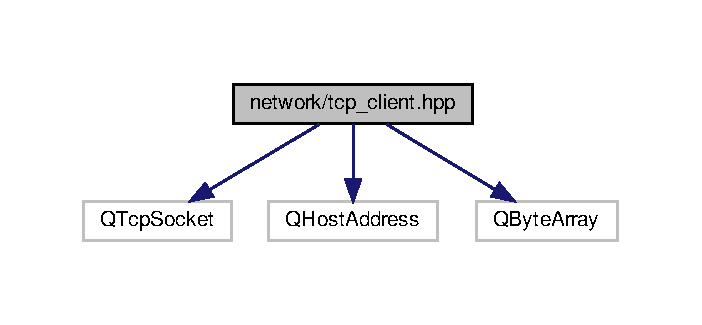
\includegraphics[width=337pt]{tcp__client_8hpp__incl}
\end{center}
\end{figure}
This graph shows which files directly or indirectly include this file\+:
\nopagebreak
\begin{figure}[H]
\begin{center}
\leavevmode
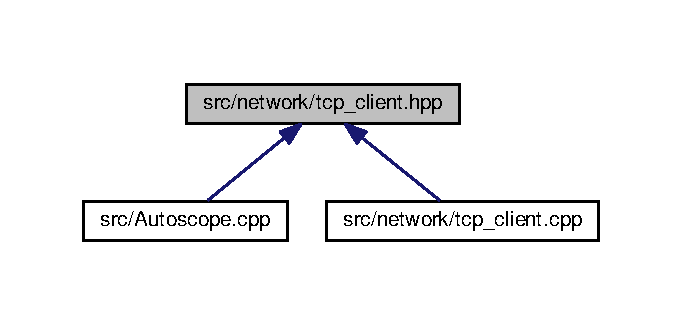
\includegraphics[width=328pt]{tcp__client_8hpp__dep__incl}
\end{center}
\end{figure}
\subsection*{Classes}
\begin{DoxyCompactItemize}
\item 
class \hyperlink{class_tcp_client}{Tcp\+Client}
\begin{DoxyCompactList}\small\item\em The \hyperlink{class_tcp_client}{Tcp\+Client} class allow to make usage of Q\+Tcp\+Socket more suitable for development. \end{DoxyCompactList}\end{DoxyCompactItemize}


\subsection{Detailed Description}
Header file including T\+CP client definition. 

\begin{DoxyAuthor}{Author}
clement-\/ailloud 
\end{DoxyAuthor}

\hypertarget{tcp__server_8cpp}{}\section{network/tcp\+\_\+server.cpp File Reference}
\label{tcp__server_8cpp}\index{network/tcp\_server.cpp@{network/tcp\_server.cpp}}
{\ttfamily \#include \char`\"{}tcp\+\_\+server.\+hpp\char`\"{}}\newline
Include dependency graph for tcp\+\_\+server.\+cpp\+:\nopagebreak
\begin{figure}[H]
\begin{center}
\leavevmode
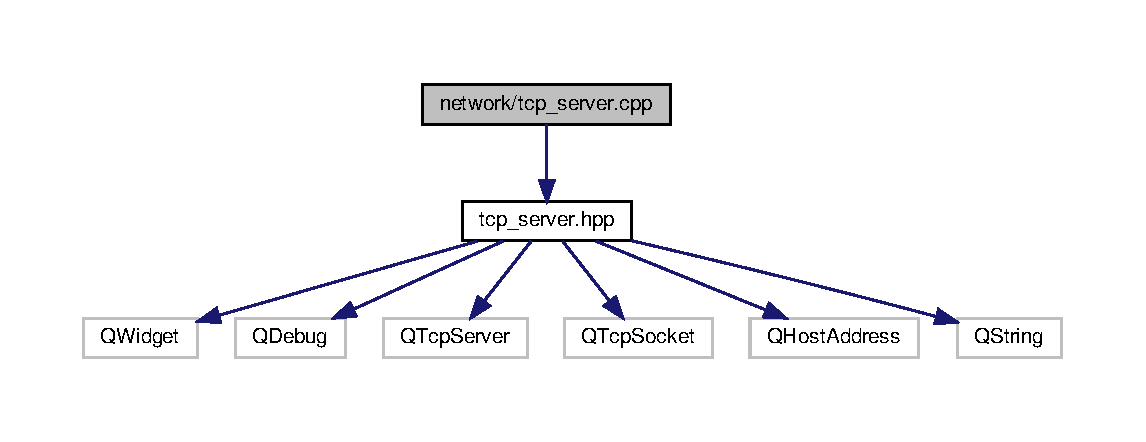
\includegraphics[width=350pt]{d4/d63/tcp__server_8cpp__incl}
\end{center}
\end{figure}

\hypertarget{tcp__server_8hpp}{}\section{src/network/tcp\+\_\+server.hpp File Reference}
\label{tcp__server_8hpp}\index{src/network/tcp\+\_\+server.\+hpp@{src/network/tcp\+\_\+server.\+hpp}}
{\ttfamily \#include $<$Q\+Widget$>$}\\*
{\ttfamily \#include $<$Q\+Debug$>$}\\*
{\ttfamily \#include $<$Q\+Tcp\+Server$>$}\\*
{\ttfamily \#include $<$Q\+Tcp\+Socket$>$}\\*
{\ttfamily \#include $<$Q\+Host\+Address$>$}\\*
{\ttfamily \#include $<$Q\+String$>$}\\*
Include dependency graph for tcp\+\_\+server.\+hpp\+:
\nopagebreak
\begin{figure}[H]
\begin{center}
\leavevmode
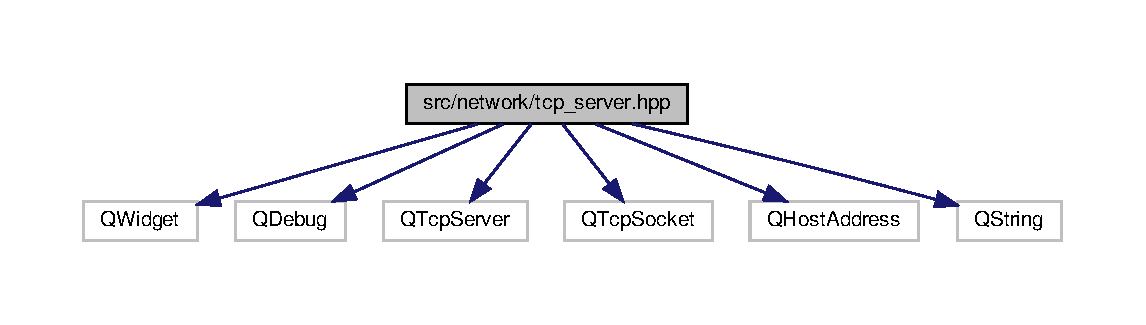
\includegraphics[width=350pt]{tcp__server_8hpp__incl}
\end{center}
\end{figure}
This graph shows which files directly or indirectly include this file\+:
\nopagebreak
\begin{figure}[H]
\begin{center}
\leavevmode
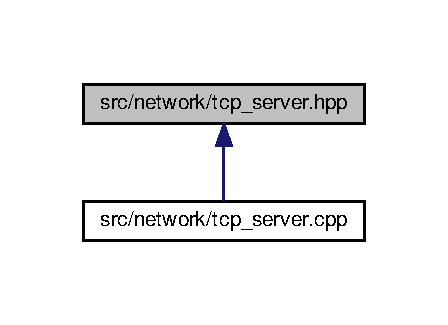
\includegraphics[width=215pt]{tcp__server_8hpp__dep__incl}
\end{center}
\end{figure}
\subsection*{Classes}
\begin{DoxyCompactItemize}
\item 
class \hyperlink{class_tcp_server}{Tcp\+Server}
\begin{DoxyCompactList}\small\item\em The \hyperlink{class_tcp_server}{Tcp\+Server} class allow to make usage of Q\+Tcp\+Server more suitable for development. \end{DoxyCompactList}\end{DoxyCompactItemize}

%--- End generated contents ---

% Index
\backmatter
\newpage
\phantomsection
\clearemptydoublepage
\addcontentsline{toc}{chapter}{Index}
\printindex

\end{document}
